\def\pre{{\text{pre}}}
\def\post{{\text{post}}}
\def\Ca{{\text{Ca}^{2+}}}

\chapter{Learning and Memory}
\label{chap:memory}

Memory and learning are so closely connected that people often confuse them with
each other. They are indeed different
\begin{itemize}
  
  \item {\bf Learning} = a process that will modify a subsequent behaviour,
  including changes in the brain strength and number of connectivities.
  
  \item {\bf Memory} = the ability to remember past experiences.
\end{itemize} 
You learn a new language by studying (i.e. a process), and you speak (i.e.
ability) by using the memory to retrieve the words that you have learned.
You learn by using one of the five senses: read (vision)/write
(touch/sensory)/listen (auditory)/smell (olfaction); and inputs via such sense
will be encoded in certain areas in the brain in some way that forms memory.

The capacity to learn, in the form of how much we can remember, is of the most
profound aspects of the human central nervous system (CNS -
Chap.\ref{chap:CNS}). So, memory is essential to all learning, in that it has
the information you learnt. Thus, memory or what is stored in the brain depends
on learning. But learning (new things) also depends on memory (the things you
learnt in the past), because the knowledge stored in your memory provides the
framework to which you link new knowledge, by {\bf association}
(Sect.\ref{sec:association-cortex}).

It has long been known that the neurons in the brains somehow encode the memory
from learning. The intriguing question is how the brain (or nerve cells) store
information (memory) at different regions in the brain. Remember that not
everything you learnt can be retrieved easily (Sect.\ref{sec:memory_brain}).

In early days, it was believed that a smarter person has more neurons which made
him/her with the capability to store more information. However, at the end of
19$^\text{th}$ century, it has been generally recognized that the number of
neurons in adult brains are pretty much the same across persons. Also, though
many (100 billion), the number does not increase significantly with age -
Sect.\ref{sec:neurogenesis}.

So learning does not need new neurons. There must be some way the brain can
encode new information using the existing neurons. It was Cajal (Spanish
neuroanatomist in 1894) proposed that memories can be formed by strengthening
the connection between existing neurons to improve the effectiveness of their
communication. \textcolor{red}{In 1949, Donald Hebb (a Canadian's psychologist)
extended Cajal's idea, and proposed that the existing neurons can}
\begin{enumerate}
  
  \item adding new connections (Sect.\ref{sec:synapse-formation}) or 
  
  \item undergo metabolic changes that enhance their ability to
  communicate, i.e. increase synaptic strength, that is, {\bf synaptic
plasticity} (Sect.\ref{sec:synaptic_plasticity}).

This is the major mechanism by which the neural activity generated by an
experience modifies brain function. However, the cellular mechanisms for this
change to occur are still under studying, and it seems there is not a single,
but many.
%is via modifications of synaptic transmission;
  
\end{enumerate}




% First, we will learn different kinds of memories in the brain
% (Sect.\ref{sec:memory_brain}). Then, we learn about synaptic plasticity
% (Sect.\ref{sec:synaptic_plasticity}).
\section{Memory in brain}
\label{sec:memory_brain}

As memory is such a fundamental concept, it is difficult yet important to
define. The general consensus is that “memory is the means by which we draw on
our past experiences in order to use this information in the present”
(Sternberg, 1999).
Or, put more simply, it is “the process of maintaining information over time”
(Matlin, 2005).

The scientific study of memory is usually traced back to Hermann Ebbinghaus
(1885/1913 translation) - one of the few experimental psychologist at that time.

Hermann is best known for his work on sensation, perception, and memory.
\begin{enumerate}
  \item sensation
  \item perception: with the famous work on optical illusion - Sect.\ref{sec:optical-illusions}
  \item memory: 

Hermann he tested on himself (over a period of 31 days) to remember and forget
new information when given a series of nonsense syllables, at different number
of times; fromn that he plotted the forgetting curve. He published the
hypothesis in 1885.
Ebbinghaus hypothesized that the speed of forgetting depends on a number of
factors such as the difficulty of the learned material (e.g. how meaningful it
is), its representation and physiological factors such as stress and sleep.

Today, we approximate forgetting with an exponential curve
\begin{equation}
R = e^{\frac{-t}{s}}
\end{equation}

with $R$ is retrievability (a measure of how easy it is to retrieve a piece of
information from memory), $S$ (stability of memory (determines how fast $R$
falls over time in the absence of training, testing or other recall), and $t$ is
time).
\textcolor{red}{IMPORTANT: Some memories remain free from the detrimental
effects of interference and don’t necessarily follow the typical forgetting
curve}.

\end{enumerate}
It has always been
challenging to know how many phases of a memory are there? Stable memorization
sometimes required further repetitions of the series.


\begin{figure}[hbt]
  \centerline{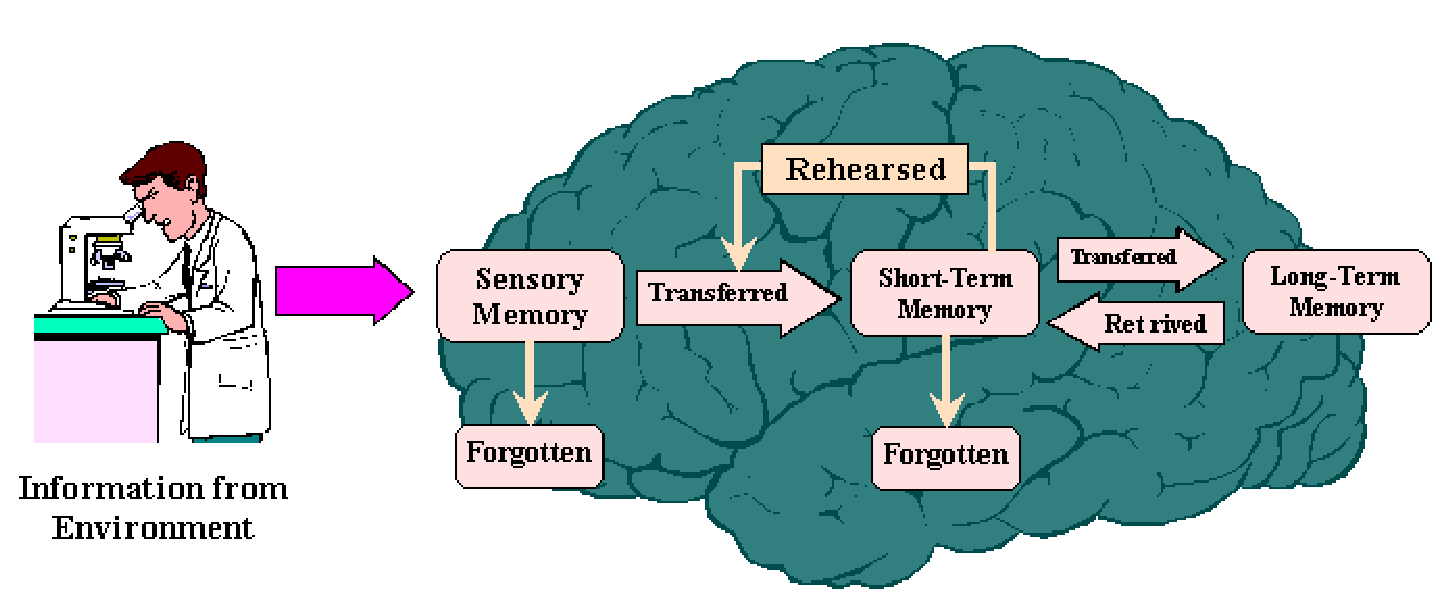
\includegraphics[height=4cm,
    angle=0]{./images/brain_store_information.eps}}
\caption{Information Processing Model (Marzano, 1998)}
\label{fig:brain_store_information}
\end{figure}

\section{Classification of memory system (1890): primary memory and secondary memory}
\label{sec:primary-secondary-memory-model}

William James (1842-1910)'s The Principles of Psychology is widely considered to
be the most important text in the history of modern psychology. He first
distinguished primary from secondary memory. For a state of mind to survive in
memory it must have endured for a certain length of time.
His work paved the way for the multi store model, a more complicated three-part
explanation of how memory processes work (Sect.\ref{sec:3-box-memory-model}).


William James (1890) proposed a distinction between {\bf primary memory} and
{\bf secondary memory}; which is similar to the concept of {\bf short-term
memory} and {\bf long-term memory}, respectively.
\begin{enumerate}
  
  \item {\bf primary memory}: the small amount of information held as the
  trailing edge of the conscious present, i.e. with consciousness.
  
  \item {\bf secondary memory}, the vast body of knowledge stored over a
  lifetime, i.e. permanent and unconscious store.
  
\end{enumerate}

Since then, it has been assumed that short-term memory processes are in charge
of cognition while long-term memory is being consolidated.

The question is \textcolor{red}{ whether short-term memory is merely a initial
phase of long-term memory, or a separate phenomena} (review: Vianna et al.
(2000) An Acad Bras Cienc).

\begin{enumerate}

  \item Several experiments, using specific molecular actions into the hippocampus, can
effectively cancel short-term memory without affecting long-term memory
formation. This shows that short-term memory and long-term memory involve
separate mechanisms and are independently processed.

  \item Other treatments, however, influence both memory types similarly,
  suggesting links between both at the receptor and at the post-receptor level,
  which should not be surprising as they both deal with nearly the same
  sensorimotor representations
\end{enumerate}
% An Acad Bras Cienc. 2000 Sep;72(3):353-64.
% Short- and long-term memory: differential involvement of neurotransmitter systems and signal transduction cascades.
% 
% Vianna MR1, Izquierdo LA, Barros DM, Walz R, Medina JH, Izquierdo I.






\section{Classification of memory system (1968): 3-box model (multi-store model,
or modal model, or Atkinson-Shiffrin model)}
\label{sec:3-box-memory-model}
\label{sec:Atkinson-Shiffrin-model}

An extension to primary and secondary memory model
(Sect.\ref{sec:primary-secondary-memory-model}) was postulated by Richard
Atkinson and Richard Shiffrin in 1968, and it remains the most
popular model for studying memory. 

It helps us consider memory as a system of information flowing through a series
of ‘stores’. They added sensory memory; and also a variety of control processes
which regulate the transfer of memory.
\begin{verbatim}

BOX 1        --->     BOX 2      ------>    BOX 3
sensory memory        short-term            long-term
(sensory register)    (working memory)
       [transition occur ....     ....   when]
       with attention>>>
                       rehersal  >>>>
                       
                       retrieval   <<<<
\end{verbatim}
With sufficient rehearsal, however, information can be encoded into the
long-term store. Once encoded in the long-term store, information can then be
transferred back to the short-term store for manipulation or processing.



This is known as {\bf three-box/three-part/information processing model},
Fig.\ref{fig:three-box-model}. Other names: {\bf modal} model or {\bf
multi-store} model or {\bf Atkinson-Shiffrin} model.
Whilst the multi store model has been influential in the field of psychology
\citep{anderson2000}, Fig.\ref{fig:brain_store_information}, it has been heavily
criticised since its publication, as it does not reflect accurately enough the
complexity of the processes involved.


\begin{figure}[htb]
  \centerline{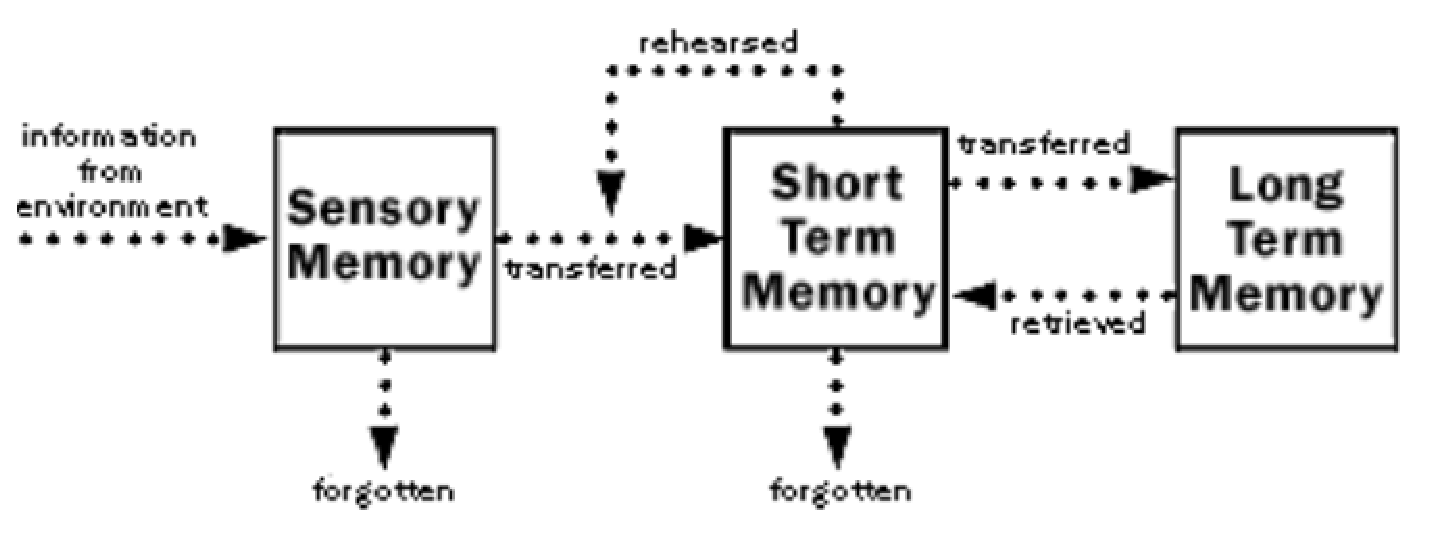
\includegraphics[height=3cm]{./images/three-box-model.eps}}
  \centerline{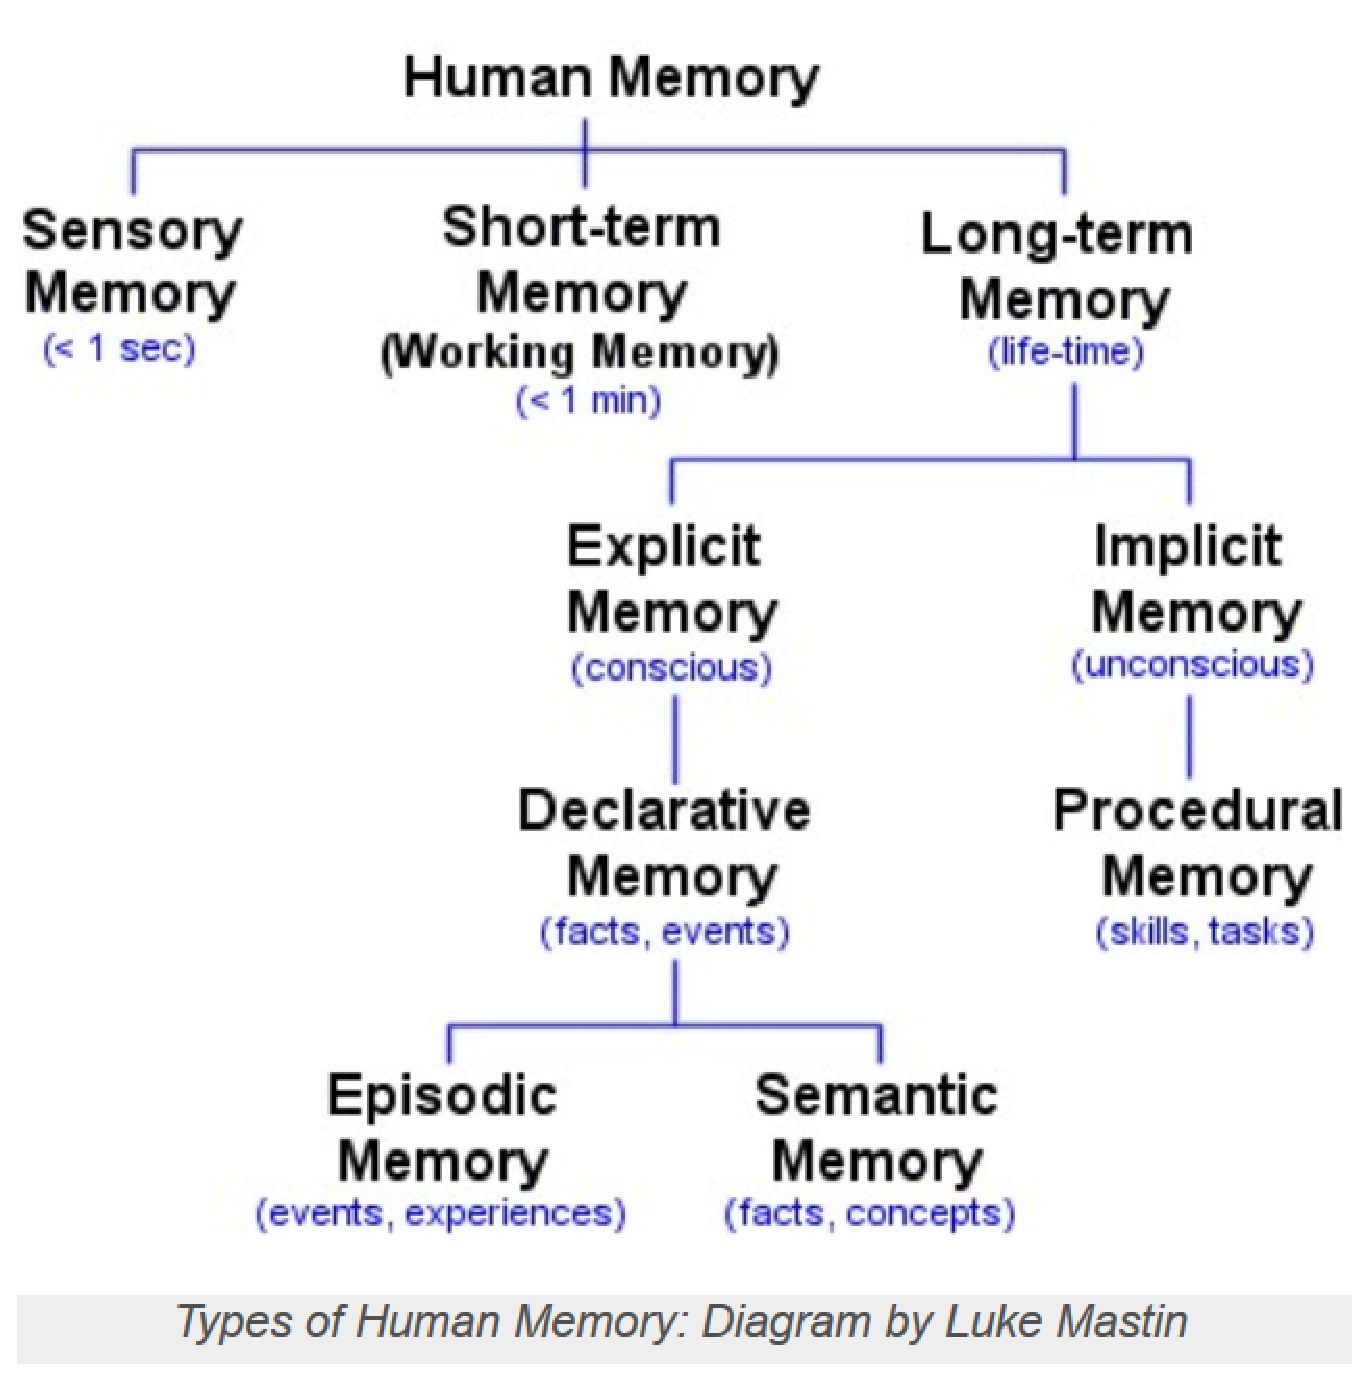
\includegraphics[height=6cm]{./images/human-memory.eps}}
  \caption{Information flow: sensory memory,
  short-term memory and then long-term memory}\label{fig:three-box-model}
\end{figure}

\subsection{-- separate STM regions}

A research subject codenamed KF suffered brain damage from a motorcycle accident
that damaged his short-term memory. His impairment was mainly verbal, whereas
his visual memory almost unaffected. This supports the view that there are
separate short-term memory components for visual and verbal information (the
visuospatial sketchpad vs. phonological loop).

\subsection{-- spatial vs visual aspect}

In a 1980 publication, Lieberman indicates that blind people are capable of high
levels of spatial awareness despite never having had any experience of visual
information. This, in effect, is a criticism of the visuospatial sketchpad, in
that it implies that spatial information is initially visual. Lieberman suggest
separating the visual and spatial aspects of this component.

\subsection{-- extended version (1974) with working memory with central executive region}

Driven to describe a more complete picture of how memory works, Alan Baddeley
and Graham Hitch proposed a model in 1974 that has come to be known as the
working memory model.

One of the more common criticisms of the working memory model is the role of the
executive function. There is little direct evidence for how it works, and
Baddeley himself acknowledges that more work needs to be done in this area.

Collating their evidence, the final model can be described as having three
separate components that feed into the central executive, the overarching
feature that monitors the other components and allocates attention:

\begin{verbatim}

i) the phonological loop, which a consists of a short-term phonological store
with auditory memory traces and an articulatory rehearsal component that can
recall those memory traces,

ii) the visuospatial sketchpad, which handles information from the senses or
from long-term memory, and

iii) the episodic buffer, which binds the information from the phonological loop
and the visuospatial sketchpad.
\end{verbatim}
The working memory model was based on both a combination of clinical evidence
(e.g. Brenda Milner’s case study on Henry Molaison) and experimental evidence
(e.g. research on differences between acoustically and semantically similar
stimulus material) throughout the late 1960s and early 1970s, which made it an
appealing theory.

% In cognitive psychology, there is one memory system, but it is normally
% divided into three functions for storage ,
\begin{enumerate}
  \item sensory memory (i.e. perception) - Sect.\ref{sec:sensory-memory}

  \item short-term memory (STM) - Sect.\ref{sec:short-term_memory}: this region
  store information that can be forgotten quickly,

  \item [2b.]working memory: 
    
Short-term memory was previously often called {\bf working memory}.
However, some considered short-term memory and working memory are different,
largely as the result of different investigators using different definition.
Many believes working memory store information for tasks of higher aptitudes
(i.e. requires much more attention). 

    \item long-term memory (LTM, often called {\bf permanent}) -
    Sect.\ref{sec:long-term_memory}: this region store information that can be
    retained in the brain for days/years.
    
The dichotomous between STM and LTM is grounded on evidence that patients with
damage to the medial temporal lobe (MTL, region containing hippocampus)
exhibited imparied LTM, but not STM  \citep{squire1992}.
\textcolor{red}{However, this viewpoint has faced considerable challenges, that
LTM and STM shares the similar underlying neural mechanism}. New data showed
that damage to MTL also affect STM involving remembering novel information, i.. 
(1) perirhinal cortex supports STM for novel object recognition, (2) hippocampus
supports STM for associative information (e.g. location of novel objects).
   
\end{enumerate}

Whilst a vast improvement on the multi store model of the late 1960s, and
generally viewed as the best understanding of memory we currently have, the
working memory model is still an incomplete picture of the processes that govern
memory.
\url{https://www.psysci.co/multi-store-model/}

\begin{mdframed}
Donald Hebb (1968) argued that it was doubtful that a chemical process could
occur fast enough to accommodate immediate memory (which is explained by
sensory memory system), yet remain stable enough to accommodate permanent
memory (i.e. can be transfer from sensory memory to STM and then LTM). This
aligns with the present theory of three storage areas.

Atkinson and Shiffrin (1968) proposed two distinct memory stores
(short-term memory + long-term memory), and then later, sensory memory was added
\url{http://users.ipfw.edu/abbott/120/AtkinsonShifrin.html}

\citep{cowan2008} emphasized three different
kinds of memory in human: long-term, short-term and working memory.
\end{mdframed}


%  Also, the memory can also be classified into recall memory
% (Sect.\ref{sec:recall-memory}) vs.
% recognition memory (Sect.\ref{sec:recognition-memory}).



% In human brain, you have short-term (Sect.\ref{sec:short-term_memory})
% and long-term memory (Sect.\ref{sec:long-term_memory}). 
\subsection{Sensory memory (perception): iconic memory, echoic memory, haptic
memory}
\label{sec:sensory-memory}

%information to store in this memory region is derived from touch, visual or
% aural.
\begin{mdframed}
{\bf HISTORY}: After you see something, a  sustained physiological image of an
object can also be 'seen' by the brain. This afterimage can be normal phenomenon
(i.e. {\it physiological afterimage}) or pathological ({\it palinopsia}).
\footnote{\url{https://en.wikipedia.org/wiki/Afterimage}} 
The existence of this {\bf visual sensory memory} and some of its
characteristics including capacity and duration was first studied by George
Sperling (1960s). This short-term memory region is coined {\bf  iconic memory}
by Ulric Neisser in 1967.

\end{mdframed}

The "sensory register" or "sensory memory" is actually composed of multiple
registers, one for each sense.  
There are three types of sensory memory: iconic, echoic and haptic;
linking to the different senses (visual, aural, or touch),
Fig.\ref{fig:brain_store_information}.

Most researches have been focusing on visual and auditory system
\begin{itemize}
  \item \textcolor{red}{\bf iconic memory (vision)} -
  Sect.\ref{sec:iconic-memory-sensory}):
  capacity (???), duration (0.5-1.0 sec), raw perceptual processing.

Sperling thought the iconic memory is discarded in less than 5 ms; yet later
agreed upon that most visual icons are eliminated from memory before 250
milliseconds.
 
  \item \textcolor{red}{\bf echoic memory (hearing)} -
  Sect.\ref{sec:echoic-memory-sensory}:
  capacity (same as that of visual system), duration (4-5sec), raw perceptual processing.
  
It is a very temporary "buffer" memory, making it possible to attend to some of
it a bit later -- as when you can still hear someone asking you a question even
though you weren't really listening when they asked it

  \item \textcolor{red}{\bf haptic memory} -
  Sect.\ref{sec:haptic-memory-sensory}:
\end{itemize}

In order for anything to enter out memory, it
must first be picked up by our senses (taste, touch, sight, hearing and smell).
This can happen very fast, as shown via {\bf free recall} experiment and {\bf
cued recall} experiment as there is no need for high-level cognitive process
involved, i.e. no information processing. 
% This first stage of memory is called {\bf sensory memory}, and there
% is no need for processing the information and thus information (stimuli) can be quickly detected.
\begin{mdframed}
Sperling (1960) famously illustrated the difference between unlimited sensory
memory and capacity-limited categorical memory.

Using a matrix 3x3 containing characters/letters, and then showed briefly to
human subject before asking he/she to recall them. This technique, called
{\bf free recall} showed that participants were able to, on average, recall 4-5
letters of the 9 they were given. Such a limit came to be known as the span of
apprehension. 

However, in a different experiment called {\bf cued recall}, it revealed that it
is not that the brain can not retains all characters in such a brief amount of time; instead,
Sperling showed that the brain had stored all of the letters in their mind
(in the region he called {\bf iconic memory}), but had simply forgotten them
while trying to recall this information on what they had seen. 

NOTE: {\bf cued recall}: recall a particular row immediately after the grid was
shown, opposed to being asked to recall the entire grid, participants
experienced higher accuracy.

%Example: register a face that you see on the street

\end{mdframed}

The retained information accurately only very briefly (i.e. from a few hundred
milliseconds to one or two seconds) that it is often considered part of the
process of {\bf perception}. Nevertheless, it represents an essential step for
storing information in short-term memory (Sect.\ref{sec:short-term_memory}).

Most of what we sense we forget almost immediately, i.e. they are not encoded in
the brain. In fact, there is just a VERY SMALL amount of information picked up
by our senses that we pay attention to and goes on to the next stage of memory
(short term memory - Sect.\ref{sec:short-term_memory}) where they are encoded.
 
% This information is only transferred to the short-term memory when attention is
% given to it, otherwise it decays rapidly and is forgotten.
% 
\subsection{-- Iconic memory}
\label{sec:iconic-memory-sensory}

\subsection{-- Echoic memory}
\label{sec:echoic-memory-sensory}

Auditory information travels as sound waves which are sensed by hair cells in
the ears. Information is sent to and processed in the temporal lobe -
Sect.\ref{sec:temporal-lobe}.

Unlike visual memory, in which our eyes can scan the stimuli over and over, the
auditory stimuli cannot be scanned over and over. Overall, echoic memories are
stored for slightly longer periods of time than iconic
memories (visual memories).

The retained period was controversial.
It is suggested retain information for 3-4 seconds before decay, which is a much
longer duration than iconic memory. Guttman and Julesz suggested that it may
last approximately one second or less, while Eriksen and Johnson suggested that
it can take up to 10 seconds

\subsection{-- Haptic memory}
\label{sec:haptic-memory-sensory}

Sensory receptors all over the body detect sensations such as pressure, itching,
and pain. Information from receptors travel through afferent neurons in the
spinal cord to the postcentral gyrus of the parietal lobe in the brain. 

fMRI studies have revealed that specific neurons in the prefrontal cortex are
involved in both SM, and motor preparation which provides a crucial link to
haptic memory and its role in motor responses.


\subsection{Short-term memory (STM: require rehersal)}
\label{sec:short-term_memory}

Sensory memory (Sect.\ref{sec:sensory-memory}) under
selective attention can move to short-term memory (STM) temporarily, i.e. it is
the ability to temporarily hold in mind information from the immediate past
(e.g., a telephone number). There are different understandings for STM (see
below).

The limited capacity of STM, George Miller suggested a capacity of 7$\pm$2 bits
of information, whereas modern estimates are as low as 4 bits (Cowan, 2001).
With sufficient rehearsal, however, information can be encoded into the
long-term store. Once encoded in the long-term store, information can then be
transferred back to the short-term store for manipulation or processing.




The term STM is related to {\bf primary memory} of James's idea published in
1890; but it is treated differently by Broadbent (1958) and Atkinson and
Shiffrin (1968) who used the term short-term memory, as they believe the term
``primary memory" might be considered to be more restricted, i.e. only in the
'conscious' state. Similarly, Cowan (2008) pointed out that short-term memory
should only hold (a limited amount of) information in a very accessible state
temporarily.  It is possible that not every temporarily accessible idea is, or
even was, in conscious awareness. For example: a person talking to a foreigner
and inadvertently alter his/her speech to match the foreign speaker's accent,
this is an unconscious aspect of short-term memory.

A similar, but can be different, concept to STM is {\bf working memory}
(Sect.\ref{sec:working-memory}).

\begin{mdframed}
NOTE: In the modeling framework, short-term memory can include sensory memory
 features - Sect.\ref{sec:sensory-memory} - as well as semantic features.

\end{mdframed} 
% Similar to sensory memory, within the STM, there can be three basic operations
% \begin{itemize}
%   \item (often) {\bf acousting memory}: hold sounds, e.g. recalling words
%   
%   \item {\bf iconic memory}: ability to hold visual images; 
% (maybe) translating images into sounds
% 
% 
%   \item  
% \end{itemize} 


There are two brain areas that share the function of storing and remembering
events for short-term memory. 

\begin{enumerate}
  \item {\bf prefrontal cortex}, especially the dorsolateral prefrontal cortex
  (dlPFC) (Sect.\ref{sec:dLPFC}) in human: known as the coordinator of
  short-term memory
  
  dlPFC plays a key role in working memory (Sect.\ref{sec:working-memory}).
  In their experiments (presentation - delay -
  response), \citep{pochon2001} (Sect.\ref{sec:delayed-response-task})
  \begin{itemize}
    \item presentation (visualspatial task): give a sequence of images
    \item delay: a short time of delay
    \item response:
    task 1 (given another sequence, and tells if they match with the one before
    the delay), task 2 (ask to reproduce the sequence)
  \end{itemize}
  
  In task 2, the subject has to  mentally organize their response during the
  delay. Interestingly, fMRI data shows that dlPFC only activates in task 2. So,
  it suggested that \textcolor{red}{parietal-premotor network is sufficient to
  store visuospatial information in STM whereas the dlPFC is involved when it is
  necessary to mentally prepare a forthcoming sequential action based on the
  information stored in STM}.
 
%   The central executive part of the prefrontal cortex at the front of the brain
%   (Sect.\ref{sec:prefrontal-cortex}) appears to play a fundamental role in
%   short-term and working memory.

  \item {\bf hippocampus} - Sect.\ref{sec:hippocampus} and share this function
  with the subiculum (Sect.\ref{sec:subiculum})
  
  Hippocampus is widely known for its role in LTM
  (Sect.\ref{sec:long-term_memory}), the recent neuropsychological data also
  shows its role in STM for association information, i.e. short-term associative
  memory task \citep{kumaran2008}. {\bf TASKS}: They test both visual and
  spatial capability to store information, i.e.
  subjects viewed a novel scene consisting of four objects (out of a set of nine
  objects), each in one of nine possible locations in a 3 x 3 grid
  (Sect.\ref{sec:delayed-matching-to-visualspatial-task})
  
  
  However, what is not clear from the neuropsychological data, however, is
  \textcolor{red}{how the hippocampus supports this STM function}. One
  possibility is that the hippocampus supports short-term memory for associative information
  through \textcolor{red}{transient changes in synaptic efficacy, rather than
  active maintenance}, as was the case in the dlPFC (Jonides et al.,
  2008).
  Alternatively, active maintenance may occur, but by a different mechanism not
  detectable by fMRI (e.g., involving theta/gamma oscillations).
  \footnote{\url{http://www.newswise.com/articles/two-brain-areas-critical-for-short-term-memory}}

\begin{mdframed}

  Hippocampus and Subiculum both 'encode' or 'remember' information, but they do
  at different times. If the imposed delay was less than 15 seconds, only the
  subiculum recorded the information. But, when the delay was longer, the
  subiculum became inactive while the hippocampus switched on and took over
  control of the memory requirements of the task.
  
  Also, when the hippocampus switched on to complete
  the trial, the memory was biased by past experience. This strategy allowed the
  hippocampus to anticipate future events based on past outcomes.

\end{mdframed}
\end{enumerate}
  

% It may register a face that we see in the street, or a telephone number that we
% overhear someone giving out, i.e. encoding: primarily acoustic , even translating
% visual information into sounds
\subsection{-- Short-term memory serial recall}
\label{sec:short-term-memory-serial-recall}	

In a test called {\bf serial recall}, a human is tested to recall the occurence
of items during a serial sequence.
It helps to understand how we store and retrieve a novel sequence of items in
the correct order, e.g. remember the phone number that we recently heard
(review: Henson, 1998).

\begin{enumerate}
  \item {\bf repetition facilitation}: in a control sequence, there is no
  repeated items; and in a testing sequence, there is a two consecutive
  occurences of the same item. 
  
  RESULT: Recall the item at the order of when the repeated occurrences occur is
  superior to recall the items at the same order in control sequence.
  
  \item {\bf repetition inhibition} ({\bf Ranschburg effect}): using the same
  control sequence, but in the testing sequence, the two occurrences of the same
  item is no longer adjacent, but are separated by a number of intervening
  items.
  
  RESULT: recall of one or both occurrences of that item is generally inferior
  to recall of two different items at corresponding positions in control
  sequences.

  \item {\bf repetition blindness}: in rapidly presented sequence, the human
  cannot detect the consecutive occurrence, i.e.  failure to detect repetition
  in rapidly presented sequences.
  
  QUESTION IS: how long of seeing an item is needed for the memory to form
  ?
  
\end{enumerate}
% repeated items are recalled; which
% shows that a person recall well when the repeated items are close together in time (repetition facilitation), but not when further apart (repetition inhibition;
% the Ranschburg effect).

The questions
\begin{enumerate}
  \item does two occurrences of the same item {\bf activate the same type of
  memory representation} or form different representations in memory ?
  (Wickelgren, 1969)
  

  \item 
\end{enumerate}

Both properties of short-term memory (as described below) are still
controversial but the current literature is rather encouraging regarding the
existence of both decay and capacity limits \citep{cowan2008}.

\begin{enumerate}
  \item {\bf limited capacity}: 7$\pm$2

Miller's (1956) published the experiment giving the so-called Magic number 7
(plus or minus two). He  thought that the short-term memory had a certain number
of ``slots" in which items could be stored. However, he did't specify the amount
of information that can be held in each slot.

Miller defined a "chunk" as an independent item of information, i.e. 
one whose recall did not aid in the further recall of the other items. 

From the different experiments on human, \textcolor{red}{short-term memory has a
storage capacity of only about seven items and lasts only a few dozen seconds}.

  \item {\bf limited duration}: 18-20 seconds (Peterson and Peterson, 1959),
  processing (information stored in STM is often encoded verbally, i.e. you need
  to repeat saying/listening to something, although other strategies may also
  be used such as visualization) - Sect.\ref{sec:memory-decay-short-term-memory}


 
\end{enumerate}


\subsection{Long-term memory (LTM)}
\label{sec:long-term_memory}

In the given 3-box memory model, just as sensory memory
(Sect.\ref{sec:sensory-memory}) is a necessary step for short-term memory,
short-term memory (Sect.\ref{sec:short-term_memory}) is a necessary step toward
the next stage of retention, long-term memory.

The use of {\bf chunking} has been proven to be a significant aid for enhancing
the STM transfer to LTM. {\small {\it Chunking = configuring large amounts of
information into smaller units of information that are scaffolded (supportive
structures) in order to accommodate memory and learning limitations}}.
\footnote{\url{http://www.nwlink.com/~donclark/hrd/learning/id/elaboration_theory.html}}

The knowledge we store in LTM affects our perceptions of the world, and
influences what information in the environment we attend to. LTM provides the
framework to which we attach new knowledge.
Long-term memory not only stores all the significant events that mark our lives,
it lets us retain the meanings of words and the physical skills that we have
learned. Its capacity seems unlimited, and it can last days, months, years, or
even an entire lifetime! However, it tends to become less reliable as we age.
An important factor for retention of learned information in LTM is rehearsal
that provides \textcolor{red}{\bf transfer of learning} - i.e. the application
of skills, knowledge, and/or attitudes that were learned in one situation to another
learning situation (Perkins, 1992). This increases the speed of learning.
\begin{itemize}
  \item near transfer: apply the skill without changing	
  \item far transfer: apply the skill, but requires adaptation (or changes)
  
  learners are trained to adapt guidelines to changing situations or
  environments.
\end{itemize}
\url{http://www.nwlink.com/~donclark/hrd/learning/memory.html}

\textcolor{red}{The information stored in STM is maintained by active firing of
neurons following some patterns; however, information stored in LTM is not
represented as patterns of neural activity (as in the case of STM), but rather
as changes in wiring} - i.e. changing the "conductivity" of existing synapses +
the formation new synapses and destruction of old ones. The recording process is
called storage and the "playback" process, retrieval.
\url{http://users.ipfw.edu/abbott/120/AtkinsonShifrin.html}

{\it There are different brain regions involving into LTM:}
\begin{enumerate}
  \item declarative memory: encoded by {\bf hippocampus}, {\bf entorhinal
  cortex}, {\bf perirhinal cortex}; while consolidated and stored in {\bf
  temporal cortex} and elsewhere
  \item procedural memory: encoded and stored by {\bf cerebellum}, {\bf
  putamen}, {\bf caudate nucleus}, {\bf motor cortex}
\end{enumerate}
More details: see below

\subsection{-- LTM: declarative (explicit)  vs.
procedural (implicit) memory}

Long-term memory can be classified into two types of LTM:
\begin{itemize}
  \item {\bf declarative memory} (explicit memory): memories of things that can
  be consciously recalled, named and described each of these remembered things
  explicitly, e.g.  facts (birthday) or knowledge (the route going home).

NOTE: While declarative memory is similar to explicit memory, declarative memory
is memory that a patient can state in words, while explicit memory is the
deliberate recall of information that the patient recognizes as a memory.

It can be divided into: episodic memory and semantic memory, and, optionally,
autobiographical memory (Sect.\ref{sec:episodic-memory}).


  \item {\bf procedural memory} (non-declarative memory, implicit memory):
  unconscious memory such as skills, e.g. learning to ride a bicycle.
  You express it by means other than words.
\end{itemize}

The two types of memories above are stored in different regions of the brain and
undergo quite different process

\subsection{----- declarative (explicit)}
\label{sec:LTM-declarative-memory}
\label{sec:declarative-memory}

\begin{itemize}
  \item episodic memory - Sect.\ref{sec:episodic-memory}
  
Optional third type:  autobiographical memory, which also holds flashbulb
memory - Sect.\ref{sec:flashbulb-memory}

  \item semantic memory - Sect.\ref{sec:semantic-memory}
\end{itemize}

{\bf declarative memory}: \textcolor{red}{encoded by}
  by the {\it hippocampus}, {\it entorhinal cortex} and {\it perirhinal cortex}
  (all within the medial temporal lobe of the brain), but are
  \textcolor{red}{consolidated and stored} in the {\it temporal cortex and
  elsewhere}.
  
  The memories of the different elements of a particular event are distributed
  in the various visual, olfactory and auditory areas of the brain, but they are
  all connected together by the {\bf hippocampus} to form an episode, rather
  than remaining a collection of separate memories. However, using hippocampus
  is not necessary in some cases, example:
  memories of people's faces, the taste of the wine, the music that
  was playing, etc, might all be part of the memory of a particular dinner with
  friends. By repeatedly reactivating or "playing back" this particular activity
  pattern in the various regions of the cortex, they become so strongly linked
  with one another that they no longer need the hippocampus to act as their
  link, and the memory of the music that was playing that night, for example,
  can act as an {\it index entry}, and may be enough to bring back the entire
  scene of the dinner party.
  
  The spatial memory, however, appears to be much more confined to the {\it
  hippocampus} (Sect.\ref{sec:spatial-memory}), particularly the right
  hippocampus, which seems to be able to create a mental map of space, thanks to
  certain cells called "place cells" (Sect.\ref{sec:place_cells}).
  
  
  Semantic memory mainly activates the {\it frontal and temporal cortexes},
  whereas episodic memory activity is concentrated in the {\it hippocampus}, at
  least initially. Once processed in the hippocampus, episodic memories are then
  consolidated and stored in the {\it neocortex}.
  
\subsection{-------- declarative memory: episodic memory (+ autobiographical
memory: flashbulb memory) + semantic memory}
\label{sec:episodic-memory}
\label{sec:semantic-memory}
\label{sec:autobiographical-memory}

(1) {\bf semantic memory} (stores a more structured records of factual
information, meanings, concepts and knowledge about the external world that a
person has acquired and is {\it independent of personal experience and of
spatial/temporal context}, e.g.
includes such things as types of food, capital cities, social customs, functions
of objects, vocabulary, understanding of mathematics, etc. Much of semantic
memory is abstract and relational and is associated with the meaning of verbal
symbols). \textcolor{blue}{The semantic memory is generally derived from the
episodic memory. A gradual transition from episodic to semantic memory can take
place, in which episodic memory reduces its sensitivity and association to
particular events, so that the information can be generalized as semantic
memory.}


(2) {\bf episodic memory} (store specific personal experience and specific
events in time in a serial form, e.g. the memory of autobiographical events
(times, places, associated emotions and other contextual knowledge) that can be
explicitly stated). 

A further category of declarative memory, referred to as (3) {\bf
autobiographical memory}, is sometimes distinguished, although really it is just
one area of episodic memory. 
One specific type of autobiographical memory is known as a "{\it flashbulb
memory}" (Sect.\ref{sec:flashbulb-memory}).

In episodic memory, whereas much research has focused on memory for the content
of an event, FMs concern memory for the source of news about that event, and
these two aspects of memory may be dissociable.

\subsection{----------- flashbulb memory}
\label{sec:flashbulb-memory}

One specific type of autobiographical memory
(Sect.\ref{sec:autobiographical-memory}) is known as a "{\it flashbulb memory}"
(FM), a highly detailed, exceptionally vivid "snapshot" of a moment or
circumstances in which surprising and consequential (or emotionally arousing)
news was heard, famous examples being the assassination of John Kennedy, the
terrorist attack on 9/11, etc.
\url{http://www.human-memory.net/types_episodic.html}

FMs appear to be more accurate and more consistent than memories for less
emotional events that occurred around the same time, although FMs are still
subject to forgetting and distortion over the long term.

Unlike other studies on episodic memory, FM research, however, is less concerned
with memory for the content (i.e. {\bf iterms} encountered in the past) than with
memory for the context in which the items were encountered, or the {\bf source}
of the information. In both cases, participants must recollect when, where,
and/or from whom they learned information.


The brain regions associated specifically with FMs remain uncertain.
Also, memories for emotional events may depend on somewhat different brain
mechanisms than memories for non-emotional events. Davidson et al. (2005)
suggested: two brain regions thought to play major roles in memory may influence
emotionally arousing public event: medial/temporal lobe/diencephalon (MTL/D) and
frontal lobe (FL). It is however, left open for future research to examine
whether specific subregions of the MTL/D or FL are differentially important for
FM.

%https://www.ncbi.nlm.nih.gov/pmc/articles/PMC2349094/
\begin{enumerate}
 
  \item Memory for content or items is usually significantly impaired by
  medial/temporal lobe/diencephalon (MTL/D - Sect.\ref{sec:temporal-lobe}) lesions,
  but is often much less affected by frontal lobe (FL) damage.

Davidson et al. (2005) suggested MTL/D group had a global impairment that
covered memory for both the central event and its source.

  \item memory for source appears to be less affected by MTL/D lesions, but more
  dependent on the FLs. 
  
  The MTL/D patients had difficulty remembering the new items, whereas the FL
  patients had no problem doing so.
  
IMPORTANT: \textcolor{red}{However, there are two reports suggesting that this
may not be the case in emotional situations}.

  \item Previous studies of emotional arousal memory in laboratory suggested
  amygdala plays a key role in FM.
  
Davidson et al. (2005) suggested similar; yet not enough data, i.e. the only a
few patients with amygdala damaged, making it is hard to examine the hypothesis.
\end{enumerate}


% \subsection{Declarative memory}
% \label{sec:declarative-memory}
% 
% Declarative memory is a type of long-term memory (Sect.\ref{sec:long-term_memory})

\subsection{---- procedural memory}
\label{sec:LTM-procedural-memory}
\label{sec:implicit-memory}
\label{sec:procedural-memory}

{\bf procedural memory}:  encoded and stored by the {\it cerebellum} (store with
timing and coordination of body skills), {\it putamen} (store skills like riding
a bike), {\it caudate nucleus} (store instinctive actions such as grooming) and
the {\it motor cortex}, all of which are involved in motor control. There is no
found involvement of the hippocampus.
  
  
Reference:
\url{http://thebrain.mcgill.ca/flash/d/d_07/d_07_p/d_07_p_tra/d_07_p_tra.html}

\subsection{-- LTM: retrospective vs. prospective}
\label{sec:retrospective-memory}
\label{sec:prospective-memory}

This classification of LTM is based on 
temporal direction of the memories.

\begin{enumerate}
  \item {\bf retrospective memory}: where the stored content is past events.
  
  It includes semantic, episodic and autobiographical memory, and declarative
  memory in general, although it can be either explicit or implicit.
  
  \item {\bf prospective memory}:where the stored content is future events.
  
  It may be either event-based or time-based, often triggered by a cue, such as
  going to the doctor (action) at 4pm (cue), or remembering to post a letter
  (action) after seeing a mailbox (cue).
  
  Event-based prospective memory involves remembering to do a certain action
  when the specific circumstances are present. Time-based prospective memory
  involves remembering to do an action at a particular point in time.
  
\end{enumerate}

Clearly, though, retrospective and prospective memory are not entirely
independent entities, and certain aspects of retrospective memory are usually
required for prospective memory.

Studies have resulted into conflict results: (1) damage in retrospective memory
affect the prospective memory, (2) impaired retrospective memory with an intact
prospective memory. The second result suggests that to some extent the two types
of memory involve separate processes.

To study the involved brain regions, they measure the regional cerebral blood
flow (rCBF) using positron emission tomography.

Brain regions:
\begin{enumerate}
  \item retrospective memory: mediotemporal lobe structures
  
  \item prospective memory: prefrontal lobe structures, \citep{burgess2001} used
  the 'delayed intention' trials (e.g. remembering to  send  a   letter  
  tomorrow   lunchtime); and they  saw an increased in rCBF in
  Brodmann's area 10 bilaterally, right lateral prefrontal and inferior
  parietal regions plus the precuneus.
  Further stimuli decreases right lateral prefrontal cortex activity, but now
  we see thalamus activation.
  
\end{enumerate}

\url{http://www.human-memory.net/types_retrospective.html}

\subsection{Factual memory}
\label{sec:factual-memory}

Factual memory can be divided into
\begin{itemize}
  \item {\bf working memory}: Sect.\ref{sec:working-memory} 
  \item {\bf reference memory}:  Sect.\ref{sec:reference-memory}
\end{itemize}


\subsection{* Reference memory}
\label{sec:reference-memory}

{\bf reference memory}:  region in the brain for remembering information
(knowledge for aspects of a task) that remains constant between trials
for a given animal (e.g., removing the cup from a baited well provides access to
food).

Originally, the term was introduced to distinguish two types of knowledge rats
may retain in a radial-arm maze task: knowledge about which arms of the maze
always contain a food reward in each trial ({\bf reference memory}) and memory
for the arms that have already been visited in search for food in the current trial
({\bf working memory} - Sect.\ref{sec:working-memory}).

How the term maps to modern concepts of human memory cannot be conclusively
determined, although, given the operational definition alone, reference memory
on a basic level resembles semantic rather than episodic memory, that is,
knowledge that is common across episodes rather than specific to a single
specific event.

Reference memory represents, like any other form of LTM
(Sect.\ref{sec:long-term_memory}), the end point of a series of processes that,
beginning with sensory transduction, attention, and encoding, result in
long-lasting behavioral changes, from which the existence of memory is inferred.
Consequently, pharmacological interventions at any point in this series of
processes can affect performance in memory tests.

\url{http://www.nature.com/npp/journal/v36/n1/fig_tab/npp2010169b1.html}

\subsection{* Working memory}
\label{sec:working-memory}

Working memory is generally used synonymously with short term
memory (Sect.\ref{sec:short-term_memory}), but the two concepts are distinct
and should be distinguished from one another (see below).

Working memory has been conceived and defined in three different, slightly
discrepant ways: 
\begin{enumerate}
  \item as short-term memory applied to cognitive tasks, 

Miller et al. (1960) used the term "working memory" to refer to {\it temporary
memory from a functional standpoint}, so from their point of view there is no
clear distinction between short-term and working memory.


  \item as a multi-component system that holds and manipulates information in
  short-term memory (Sect.\ref{sec:short-term_memory}), and 

Baddeley and Hitch (1974) made a distincsion between short-term memory and
working memory (Sect.\ref{sec:working-memory}). They believed that in a
multi-component system that could not be reduced to a unitary short-term store,
they used the term working memory to describe that entire system.
  
  \item as the use of attention to manage short-term memory.

{\bf NEWER DEFINITION}: Since then, there has been some shift in the definition
of working memory so that newer working memory task correlate with intelligence
and aptitude measures so much more highly than simple, traditional, short-term
memmory tasks such as serial recall.

New definition allows the simple statement that working memory correlates highly
with aptitudes, whereas short-term memory (redefined to include only the
non-attention-related aspects of memory storage) does not correlate so highly
with aptitudes.
\end{enumerate}

  
% {\bf working memory}: region in the brain for remembering information that
% varies unpredictably in time and/or in content.

Working memory is a theoretical framework that refers to structures and
processes used for temporarily storing and manipulating information.
Working memory include a subsystem in the brain that store and manipulate visual
images or verbal information.
These processes are sensitive to age: working memory is associated with
cognitive development, and research shows that its capacity tends to decline
with old age. Using different tests (Sect.\ref{sec:test-training-memory}), it
has been widely accepted that the 
\begin{itemize}
  \item dLPFC is the region that implements processes critical for organizing
  items in working memory (Sect.\ref{sec:dLPFC}), based on neuroimaging studies.

\end{itemize}
  
It is this type of memory that is decimated in Alzheimer's disease and other
dementias. The study of working memory processes is generally accomplished using
{\it delayed response (DR) tasks} and, within the confines of even relatively
short test sessions, one can readily assess processes associated with {\bf
short-term memory} using these procedures.
\url{http://www.simplypsychology.org/short-term-memory.html}


  
%\section{Hebbian synapse}


\section{Classification of memory system  (1972): levels-of-processing model}
\label{sec:level-of-processing-model}

Instead of thinking of memories as long-term of short-term, this model looks at
them as how deeply they have been processed, i.e. whether they are deeply
(elaborately) processed or shallowly (maintenance) processed.
The levels of processing model (Craik and Lockhart, 1972) focuses on the depth
of processing involved in memory, and predicts the deeper information is
processed, the longer a memory trace will last.


It was developed by Fergus Craik and Robert Lockhart in 1972, and posits that
memory recall, and the extent to which something is memorized, is a function of
the depth of mental processing, on a continuous scale from shallow (perceptual)
to deep (semantic). Under this model, there is no real structure to memory and
no distinction between short-term and long-term memory.
The deeper the level of processing, the easier the information is to recall.

Memory is just a by-product of the depth of processing of information, and there
is no clear distinction between short term and long term memory. Information is processed in 3 ways
\begin{enumerate}
  \item   Structural processing (appearance) which is when we encode only the physical qualities of something.  E.g. the typeface of a word or how the letters look.
  
  \item  Phonemic processing – which is when we encode its sound.
  
  \item Semantic processing, which happens when we encode the meaning of a word and relate it to similar words with similar meaning.
  
\end{enumerate}

In that the first two forms are part of {\bf Shallow Processing}; and the third
form is the {\bf Deep Processing}.
Deep processing involves elaboration rehearsal which involves a more meaningful
analysis (e.g. images, thinking, associations etc.) of information and leads to
better recall.


If you repeat something over and over again to yourself, take a quiz on it- do
well, but forget it soon after- that information was shallowly (maintenance)
processed in memory.  If you give the information meaning while memorizing it
(for example, relate it to your life or talk about it with friends) than you
should deeply (elaborately) process the information and it will last much longer
in your memory.

The levels of processing model changed the direction of memory research. It
showed that encoding was not a simple, straightforward process. This widened the
focus from seeing long-term memory as a simple storage unit to seeing it as a
complex processing system.


Despite these strengths, there are a number of criticisms of the levels of processing theory:
\begin{enumerate}
  \item  It does not explain how the deeper processing results in better memories. 
  
  \item Deeper processing takes more effort than shallow processing and it could
  be this, rather than the depth of processing that makes it more likely people
  will remember something.
  
  \item The concept of depth is vague and cannot be observed. Therefore, it cannot be objectively measured. 
\end{enumerate}
Eysenck (1990) claims that the levels of processing theory describes rather than explains. 
The ideas of 'depth' and 'elaboration' are vague and ill defined (Eysenck, 1978). 
As a result, they are difficult to measure. Indeed, there is no independent way of measuring the depth of processing.
\url{https://www.simplypsychology.org/levelsofprocessing.html}
\url{https://www.researchgate.net/publication/11066090_Levels_of_processing_Past_present_and_future}

Later research indicated that processing is more complex and varied than the
levels of processing theory suggests, i.e. there is more to processing than depth and elaboration.

For example, research by Bransford et al. (1979) indicated that a sentence such
as, 'A mosquito is like a doctor because both draw blood' is more likely to be
recalled than the more elaborated sentence, 'A mosquito is like a racoon because
they both have head, legs and jaws'. It appears that it is the distinctiveness
of the first sentence which makes it easier to remember - it's unusual to
compare a doctor to a mosquito. As a result, the sentence stands out and is more
easily recalled.


\section{Retrieval of memory}

Getting the information out of our heads so we can use it is a pretty important
part of memory.  There are basically two main types of retrieval; recognition
(Sect.\ref{sec:recognition-memory}) and recall (Sect.\ref{sec:recall-memory}).

\subsection{How memory is accessed?}

In humans, memory is often accessed through spoken or written language, while in
animals, cognitive functions must be accessed through different kinds of
behaviors in many specific, experimental models of memory and learning
(Sect.\ref{sec:test-training-memory}).


\textcolor{red}{Note that some of the terms described in this section were first
derived from animal trials, but not for human}. A basic dichotomy distinguishes
between the retention of {\bf factual or experiential information} on the one
hand, and the retention of {\bf habits and motor skills} on the other.

\subsection{Recognition memory}
\label{sec:recognition-memory}

Strictly speaking, recognition is a process of memory retrieval.
But how a memory is formed in the first place affects how it is retrieved. 

There are two component processes:
\begin{itemize}
  \item {\it recollection} (remembering, knowing): retrieval the details of the
  event that was previously experienced. This process is slower.
  
  \item {\it familarity}: feeling the event that was previously experienced,
  without knowing the details. Thus, this process should be fast, automatic.
\end{itemize}

Essentially, recognition memory refers to a brain region that store information
of previously encountered events, objects, or people. It is a subcategory of
{\it declarative memory} (Sect.\ref{sec:declarative-memory}).


\url{http://en.wikipedia.org/wiki/Recognition_memory}

\subsection{Recall memory}
\label{sec:recall-memory}

It takes longer to retrieve the information stored in the recall memory.
So, \textcolor{red}{recognition is easier than recall}
(Sect.\ref{sec:recognition-memory}).

%Recall is also a process of memory retrieval. 
The anterior cingulate cortex, globus pallidus, thalamus, and cerebellum
(Sect.\ref{sec:cerebellum}) show higher activation during recall than during
recognition which suggests that these components of the cerebello-frontal
pathway play a role in recall processes that they do not in recognition.

There are three main types of recall: free recall, cued recall and serial
recall. Two main theories of the process of recall are the {\bf Two-Stage
Theory} (Austin Simonson theory - Sect.\ref{sec:two-stage-theory}) and the {\bf theory of
Encoding Specificity} (Sect.\ref{sec:theory-of-encoding-specificity}).

\subsection{item memory}
\label{sec:item-memory}

While frontal lobes has been showed to be important in source memory
(Sect.\ref{sec:source-memory}), medial temporal lobe showed important in
recall of the actual items.

\subsection{source memory}
\label{sec:source-memory}

{\bf Source memory} refers to recalling (Sect.\ref{sec:recall-memory}) the
source of learned information, such as knowledge of when or where something was
learned. Often, memories are triggered by contextual information (i.e., time and
place).

Source memory failure may be associated with old age, stress, distractibility,
or intoxication and is a phenomenon in which a person retrieves fragments of a
memory without remembering how or when the fragment was acquired. Source memory
impairments have been shown to be disproportionately impaired in patients with
frontal lobe lesions, e.g. in studying of flashbulb memory
(Sect.\ref{sec:flashbulb-memory}).

% For instance, when asked to learn two separate lists of items, frontal lobe
% patients are impaired at determining if a word was on the first or second list
% (i.e., source), and not on the actual recall or recognition of the items. In
% contrast, medial temporal amnesics are impaired in recall of the actual items
% but no ..




\subsection{How memory is stored and decay? time-based theories vs.
interference-based theories}

\begin{itemize}

  \item Many believe temporal decay is the primary mechanism of memory loss in
  STM (Sect.\ref{sec:short-term_memory}).
  
  \item However, McGeoch (1932) illustrated that forgetting over time was not
  simply a matter of an inevitable decay of memory but rather of interference
  during the retention interval, such that  one could find situations in which
  memory improved, rather than diminish, over time (review:
  \citep{lewandowsky2004}) in the context of {\it short-term serial call}
  (Sect.\ref{sec:short-term-memory-serial-recall}).

  According to Atkinson and Shiffrin (1971), it  can be lost with the
  distraction or passage of time (15-30 seconds). So, from this perspective,
  forgetting from primary memory is considered as the profound effect of
  interference from other items on memory for any one item,
with interference effects continuing forever but not totally destroying a given
memory.
   
\end{itemize}   

% McGeoch (1932) illustrated that forgetting over time was not simply a matter of
% an inevitable decay of memory but rather of interference during the retention
% interval; one could find situations in which memory improved, rather than
% diminish, over time (review: \citep{lewandowsky2004}) in the context of {\it
% short-term serial call} (Sect.\ref{sec:short-term-memory-serial-recall}).


If memory is maintained, the question is how and how long it is maintained;
before decaying starts?

\subsection{-- short-term memory}
\label{sec:memory-decay-short-term-memory}

\textcolor{red}{MECHANISM OF DECAY}: the duration 18-20 seconds assumes that the
information is not being actively rehearsed (Sect.\ref{sec:short-term_memory}).

Information that is being actively attended to is represented by a pattern of
neural activity in the brain may become represented more permanently by guiding
changes in neural connectivity in the brain, a process referred to as storage.
But information that is not more permanently stored is simply lost shortly after
attention is directed elsewhere.
  
So, one might relate short-term memory to a pattern of neural firing that
represents a particular idea and one might consider the idea to be in short-term memory
only when the firing pattern, or cell assembly, is active.
It is an active process to keep some information until it is put to use (a
process known as {\it rehearsal}, Fig.\ref{fig:brain_store_information}).

Note that the goal is not really to move the information from STM to LTM, but
merely put  the information to immediate use. Example:  (think of a phone number
 you'll repeat to yourself until you can dial it on the phone).
NOTE: this information will quickly disappear forever unless we make a conscious
effort to retain it.
STM works like computer RAM, i.e. a working space for short computation and then
the data is either transferred to other parts of the memory system, or discard
it. STM is vulnerable to interruption or interference.

\section{Rewarding system}
\label{sec:reward-system}

% TODO: add rewarding system
A key component to rational decision-making and appropriate goal-directed
behaviors is the ability to evaluate reward value, predictability, and risk
accurately. The {\bf reward circuit}, central to mediating this information and
to assessing the likely outcomes from different choices effectively, is a
complex neural network. The center of this network is the cortico-ventral
basal ganglia (BG) circuit; and the reward circuit is embedded within this
system and is a key driving force for the development and monitoring of these
behaviors.

\begin{enumerate}

  \item  hypothalamus and other subcortical structures are involved in
  processing information about basic, or primary, rewards, 
  
  \item higher-order cortical and subcortical forebrain structures are engaged
  when complex choices about these fundamental needs are required. 

choices often involve secondary rewards, such as money, power, or challenge,
that are more abstract (compared to primary needs).
\end{enumerate}

COMPONENTS: orbitofrontal cortex (OFC) and anterior cingulate cortex (ACC), the
ventral striatum (VS) - Sect.\ref{sec:ventral-striatum}, the
ventral pallidum (VP), and the midbrain dopamine (DA) neurons.

\chapter{Mechanism of illusions}

\section{Optical illusions}
\label{sec:optical-illusions}

\textcolor{red}{\bf Ebbinghaus illusion} (or  Titchener circles) \url{https://en.wikipedia.org/wiki/Ebbinghaus_illusion}
is about size illusion:
\begin{enumerate}
  \item  two circles of identical size are placed near to each other, 
  one is surrounded by large circles while the other is surrounded by small circles
  
  As a result of the juxtaposition of circles, the central circle surrounded by
  large circles appears smaller than the central circle surrounded by small
  circles.


  \item
\end{enumerate}

Recent studies believed the two important factors: distance of the surrounding
circles from the central circle and the completeness of the annulus
 

\textcolor{red}{\bf Delboeuf illusion}:




\chapter{Neuroplasticity: Cellular and Mollecular processes underline learning
and memory formation}
\label{sec:source-synaptic-plasticity}

So, we have learnt different forms of memory in the brain
(Sect.\ref{sec:memory_brain}), e.g. long-term, short-term, each is
stored/regulated by one or different parts of the brain.
{\bf The question is what is the cellular and mollecular processes that
underlying the formation of memory and the capability of learning?} ANSWER: The
change in the brain, at neuron level is called {\bf neuroplasticity} which is
the ability of a particular part or region of a neuron to change in strength
over time.

Neuroplasticity is largely categorized into 2 groups
%There are different proposed mechanisms:
\begin{enumerate}
  \item {\bf synaptic plasticity} (i.e. the changes occur at the synapse) -
  Sect.\ref{sec:synaptic_plasticity}.
  
  
  \item {\bf non-synaptic plasticity} (i.e. the intrinsic changes occur at the
  locations fart from the synapses, e.g. axon, soma and also dendrites)
  - Sect.\ref{sec:nonsynaptic-plasticity}.
 
 
\end{enumerate}

Nonsynaptic and synaptic plasticity have been shown to work concurrently in a
variety of ways to produce stimulating effects in the neuron, e.g.
\begin{itemize}
  \item  Nonsynaptic dendritic plasticity also adds to the effects of synaptic
  plasticity through widening of the action potential
  
  \item brain-derived neurotrophic factor (BNDF) is produced by neurons to
  coordinate nonsynaptic and synaptic plasticity - Sect.\ref{sec:BDNF}
\end{itemize}


\subsection{Non-synaptic plasticity}
\label{sec:nonsynaptic-plasticity}

NOTE: nonsynaptic plasticity is a less well known and somewhat new and ongoing
field of research in neuroscience. Nonsynaptic plasticity can have short-term
or long-term effects. The reason for having non-synaptic plasticity is that
it is suggested taht synapses are not the only aspect of neurons that can adapt
and change in response to spiking behavior.
  
Nonsynaptic plasticity refers to the modification of the intrinsic
excitability of the neuron at regions away from spines, through e.g.
\begin{enumerate}
  \item modification of voltage-gated ion channels


  
  \item
\end{enumerate}  
which affects the firing threshold, a neuron's tendency to fire in bursts, the
ratio of excitatory to inhibitory receptors, the duration of its refractory
period, and its tendency to grow new dendrites or synapses.

It interacts with synaptic plasticity, but it is considered a separate
entity from synaptic plasticity.
Nonsynaptic changes in the somal body, axon, or dendrites of the neuron are
inextricably linked to synaptic strength.

Compared to synaptic plasticity (Sect.\ref{sec:synaptic_plasticity}),
nonsynaptic plasticity is a less well known and somewhat new and ongoing field
of research in neuroscience.

\url{https://en.wikipedia.org/wiki/Nonsynaptic_plasticity}

\subsection{Synaptic plasticity}
\label{sec:synaptic_plasticity}

Synaptic plasticity refers to the capability of changing synaptic strength of a
synapse after some ``modification''
\begin{itemize}
  \item at that synapse: it is called {\bf homosynaptic plasticity}
  \item at a different (probably neighboring) synapse: it is called {\bf
  heterosynaptic plasticity}
\end{itemize}

A neuron usually receives synapses from thousands of other neurons, and many of
those inputs may be synchronously active.
The way in which postsynaptic cells integrate these numerous inputs and alters
its own electrical activity is the fundamental basis of neuronal integration,
information processing, and storage in the brain.

{\bf Induction phase} refers to the time for such ``modification" to be
initiated (what kind of modification will be discussed later).
Suppose the synapse response with a given postsynaptic output (e.g. EPSC -
Sect.\ref{sec:EPSC}) for a given input pattern. After a time period of
``induction phase'', over time these synapses become increasingly sensitive to
the same input pattern, i.e. the postsynaptic output is now much stronger, or
less sensitive to the same input patter, i.e. the postsynaptic output is
weaker.
 
Virtually all types of synapses are regulated by a variety of short-lived and
long-lasting processes, which can leads to the increase or decrease in synaptic
strength (weight). To know if there is a change, we need to understand how the
synaptic strength is measured (Sect.\ref{sec:synaptic-strength-measure}).
  
There are two parts: (1) how fast the change can occur, and (2) how long the
change can sustain.
\begin{enumerate}
  \item (1):  The two general forms of synaptic plasticity that operates
on 2 different time scales
\begin{enumerate}
  
  \item non-homeostasis synaptic scaling (short-term plasticity, long-term
  plasticity LTP/LTD) - {\bf extrinsic}:
  rapid adjustment of the synaptic strength of individual synapses in responses
  to specific pattern of correlated synaptic activity.
   This is typically brought
  about by the Hebb rule ``correlated activity'': {\it when the presynaptic and
  the postsynaptic neurons are active simultaneously, their connections become
  strengthened}.
    
  \item Homeostasis synaptic scaling (upscaling and downscaling) -
  Sect.\ref{sec:homeostatic-plasticity} - {\bf intrinsic}:
  entails uniform adjustment in the strength of all synapses on a cell in response to
   prolonged change in the cell's electrical activity.
\end{enumerate}

\begin{mdframed}
\textcolor{red}{\bf Intrinsic vs. Extrinsic}:
At the higher level, synaptic plasticity is classified based on the intrinsic or
extrinsic nature of the source.
\begin{itemize}
  \item {\bf intrinsic synaptic plasticity} (homosynaptic mechanisms,
  homeostatic plasticity):  changes in the strength of a synapse that are brought about by its own
   activity. %Sect.\ref{sec:STplasticity} 
   
 
   
%    There are two types of them
%    \begin{enumerate}
%      \item intrinsic synaptic depression: STD
%      \item intrinsic synaptic facilitation (potentiation): STP
% % it is indeed an extreme example of facilitation (above), i.e.
% % a short-lived.
% \url{http://en.wikipedia.org/wiki/Post-tetanic_potentiation}
%   \end{enumerate}
%    \textcolor{red}{Some synapses exhibit one but not the other, whereas some
%    synapses exhibit both.} 
  
  \item {\bf extrinsic synaptic plasticity} (heterosynaptic plasticity):
   change in the strength of a synapse brought about by activity from
   outside, i.e. the network activity. %Sect.\ref{sec:LTplasticity}
   
%    There are two types of them
%    \begin{enumerate}
%      \item extrinsic synaptic depression: LTD
%      \item extrinsic synaptic facilitation: LTP
%    \end{enumerate}
\end{itemize}
% \textcolor{red}{We will focus on intrinsic synaptic plasticity}
% (Sect.\ref{sec:HmSP}).
\end{mdframed}

  \item (2): we focus on non-homeostasis synaptic scaling:


This change (increase or decrease) in synaptic efficacy at a
single neuron can sustain for short or long period of time, and is considered as
the underlying mechanism for storing memory in the brain
(Sect.\ref{sec:memory_brain}). This change can be maintained for short-time or
long-time, both as an increase or a decrease in plasticity. This leads to many
terms
\begin{itemize}
  \item If the change is sustained for a long period of time, it is called
  long-term plasticity (Sect.\ref{sec:LTplasticity})
\begin{enumerate}
 
  \item long-term depression (LTD):
  
  \item long-term potentiation (LTP)

\end{enumerate}
  
  \item If the change is sustained for a short period of time, it is called
  short-term plasticity (Sect.\ref{sec:STplasticity})
\begin{enumerate}
  \item short-term depression: the decrease in plasticity and it is maintained
  for short time ()
  
  \item short-term potentiation (STP):
 \end{enumerate}
\end{itemize}  
\end{enumerate}


Then, {\bf the next question is how the plasticity change occurs, i.e.
source of synaptic plasticity?} 
Elucidating the detailed molecular mechanisms underlying synaptic plasticity in
any number of different brain regions is critical for understanding the neural
basis of many aspects of normal and pathological brain function.

ANSWER: For the case of non-homeostasis synaptic scaling, there are several
proposed mechanisms for this synaptic modification to occur, depending whether
it is potentiation (STP, LTP) or depression (STD, LTD) and which regions of the
brain.
\textcolor{red}{Mainly, we focus on the different mechanism leading to LTD and
LTP}. Each neuron types can potentially possess one or many of the given
mechanisms. Different induction protocols have been used to provide some
insights into the underlying cellular mechanisms.




% To understand how to model synaptic plasticity, read
% Sect.\ref{sec:synaptic_plasticity_model}.

% \subsection{Synaptic modification: Hebbian + anti-Hebbian +
% non-Hebbian synaptic modification}

% \subsection{Pre-Hebbian theories}


\section{Non-synaptic plasticity}


\subsection{Homeostatic-plasticity}
\label{sec:homeostatic-plasticity}

Homeostatic-plasticity refers to self-stabilizing mechanism of the neurons at
regions away from the spines. A similar mechanism, that occur at the synapse is
called homeostatic synaptic plasticity
(Sect.\ref{sec:homeostatic-synaptic-plasticity}).

  
  It is reasonable to assume that there must be mechanisms to keep spike rates
  within some reasonable range. While those mechanisms are not fully known,
  possibilities include downregulation of the total number of AMPA receptors,
  upregulation of the total number of GABA receptors, increase in the inhibitory
  potassium leak current, upregulation of the spiking threshold, or molecular
  changes to increase the duration of the refractary (reset) period.
  
  

\section{(What cause) synaptic plasticity}

\begin{enumerate}
  \item Pre to Post:
  
  \item Post to Pre: retrograde signaling - Sect.\ref{sec:retrograde-signaling-pathway}
  
  \item Post to Post ?
  
  \item Pre to Pre ?
  
  \item Glial cells to Pre ?
  
  \item Glial cells to Post ?
\end{enumerate}


\section{(Forms of) synaptic plasticity}


 structural plasticity, i.e.
  the structural change at the postsynaptic sites on dendritic spines, e.g. removing existing or forming new synapses, or
  existing synapse shrink or growth.
  
% It has been widely accepted the change in synaptic plasticity
% (Sect.\ref{sec:synaptic_plasticity}) is the cellular mechanism for the formation
% in memory. 

\begin{mdframed}
\textcolor{red}{HISTORICAL FACTS: Pre-Hebbian theories}

To explain the phenomenon such as how does a man come, after having thought of
A, to have the thought of B the next moment or always together as pointed out by
James in 1890, Jame's law of neural habbit: {\it when two elementary brain
processes have been active together (or in immediate succession), one of them,
on recurring, tends to propagate its excitement to another} - an
activity-modification relationship.

Then, the term 'neuron' is substituted for elementary brain processes, and the
location for the activity-based modification is believed to occur at the
synapse. Wood-Jones and Porteus (1928) proposed the linkage at two side of a
synapse must be {\bf plastic}. It works like a resistor in an electric circuit,
with the resistance can be
\begin{itemize}
  \item lowered for the passage of the impulse from presynaptic to postsynaptic
  side easier. This is called {\bf facilitation}.

Nowadays, we call it {\bf increase synaptic conductance} (or {\bf increase
synaptic effiency}), instead of lowering synaptic resistance.
  
  \item increased for making a weak response
  
\end{itemize}
In the neuron, with plasticity, given the same presynaptic input, the
postsynaptic signal, once activated, can be higher or lower than normal.
However, Wood-Jones and Porteus did not elaborate the conditions that trigger or
induce the enhanced synaptic efficacy. 

Jerzy Koznorski (1948) extended the association theory and assumed that {\it
when the excitation of a given center is synchronous with the rise of excitation
in another center, conditioned excitatory connexions are formed the first of
these centers to the latter}. In 1949, Hebb is the first one to propose a
hypothesis about the mechanism for synaptic plasticity enhancement; yet not
with plasticity depression (Sect.\ref{sec:Hebbian-theory}).


\end{mdframed}
\subsection{Structural plasticity}
\label{sec:structural-plasticity}
\label{sec:plasticity-structural}

Structural plasticity refers to the change to the structure of the branches,
e.g. levels of dendritic arbors, to help maintain the same excitability of the
neurons.

Example Zhao et al. 2016: 
``Here, we demonstrate that over-expression of dopamine D2 receptors in medium
spiny neurons increases their membrane excitability and decreases the complexity
and length of their dendritic arbors. These changes can be reversed in the adult
animal after restoring D2 receptors to wild-type levels, demonstrating a high
degree of structural plasticity in the adult striatum. Increased excitability
and decreased dendritic arborization are associated with down-regulation of
inward rectifier potassium channels (Kir2.1/2.3).



\subsection{- Short-term plasticity: STD + STP + PTP}
\label{sec:STplasticity}
\label{sec:short-term_potentiation}
\label{sec:short-term_depression}
\label{sec:post-tetanic-potentiation}



Short-term synaptic plasticity, Fig.\ref{fig:STplasticity} acts on a timescale of tens of
milliseconds to a few minutes, unlike long-term plasticity
(Sect.\ref{sec:LTplasticity}), which lasts from minutes to hours or even years.

Short term plasticity can either strengthen or weaken a synapse, as seen in a
pair-pulse protocol (Sect.\ref{sec:pair-pulse-ratio}) within 100ms interval.
\begin{itemize}
  \item strengthen: is called {\bf synaptic enhancement}
  \item weaken: is called {\bf synaptic depression} (synaptic fatigue), i.e.
  the depletion of the readily releasable vesicles
\end{itemize}

\begin{figure}[hbt]
  \centerline{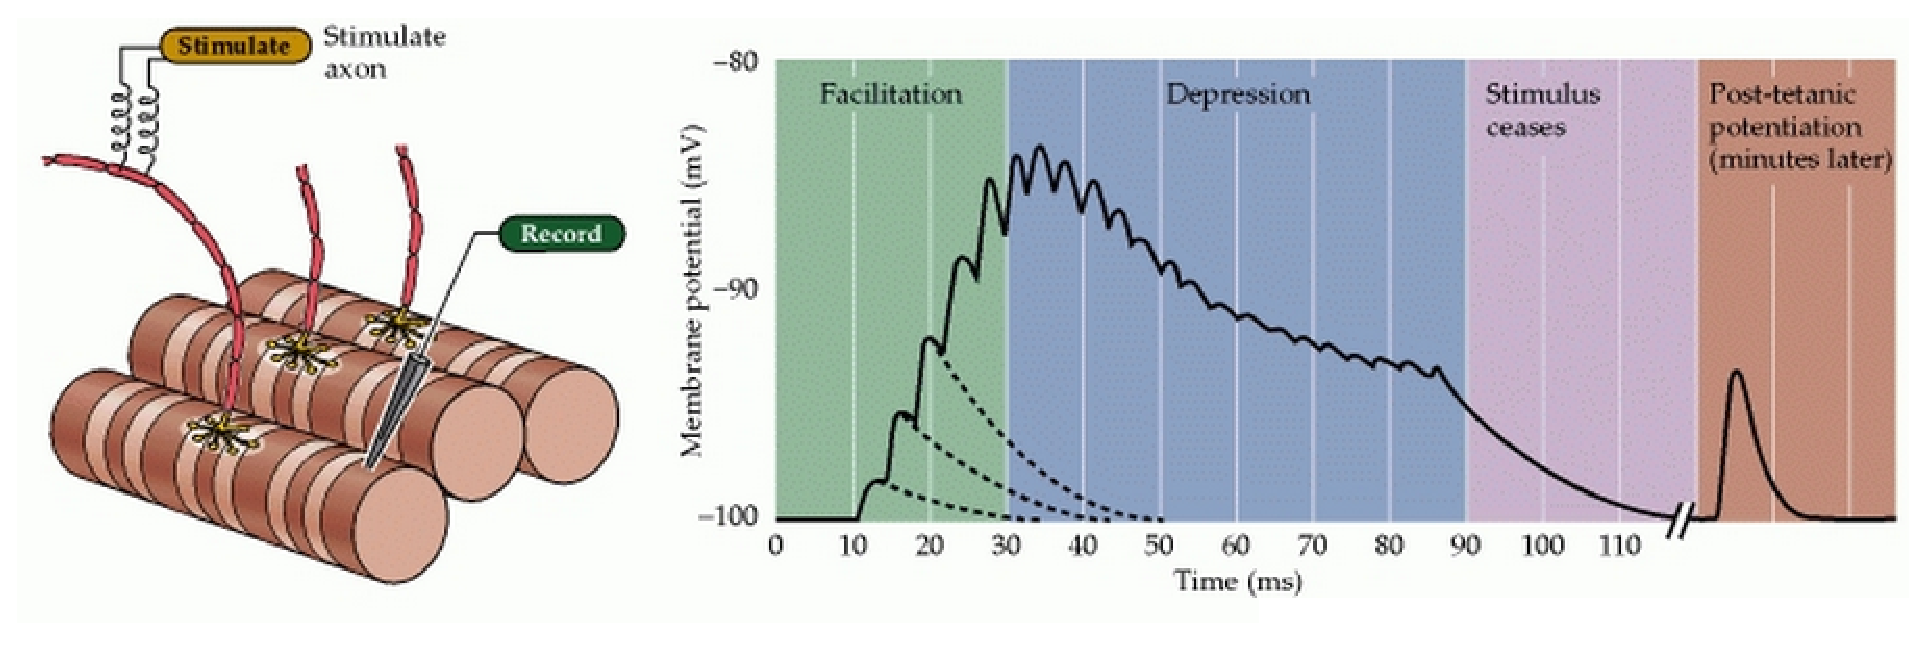
\includegraphics[height=5cm,
    angle=0]{./images/STplasticity.eps}}
\caption{Short-Term Plasticity in neuromuscular junction. (A) Facilitation
via the increased in EPP as a result of the repeated activation from the
neuro-side. (B) If the presynaptic activation continues, depression occurs
following facilitation (this is explained by the depleting of
neurotransmitter); (C) Once the train of stimulus end, the EPP also go back to
the resting level; (D) However, following this rapid train of stimulus, somehow
it affects to the synapse excitability (enhancement or depression) to a future
AP - here we see an enhancement called post-tetanic potentiation (PTP)}
%http://www.ncbi.nlm.nih.gov/books/NBK10968/
\label{fig:STplasticity}
\end{figure}

Depending on the time-scale of the change, and the trend of the change
(increase or decrease) of synaptic efficacy (Sect.\ref{sec:synaptic-strength}),
there are different terms are used:
short-term synaptic facilitation, depression, augmentation, and potentiation.

Using pair-pulse protocol, i.e. the stimulus is always from presynaptic side, in
\textcolor{red}{short-term plasticity}, and the plasticity can be regulated by
mainly from \textcolor{red}{presynaptic side} \citep{fioravante2011,
regehr2012}.
\begin{enumerate}
  \item enhanced presynaptic $\Ca$ level: \textcolor{blue}{lead to short-term
  facilitation}
  
  \item presynaptic vesicle pool: Sect.\ref{sec:synaptic-vesicles}
    \textcolor{blue}{lead to short-term facillitation}.
    
\end{enumerate}
but can be \textcolor{red}{postsynaptic factors} which can complicate
the characterization of presynaptic mechanisms 
\begin{enumerate}
    \item saturation of postsynaptic receptors can limit responses
    (particularly when the probability of release is high):
    
To minimize the saturation on AMPAR in glutamatergic synapses
(Sect.\ref{sec:glutamatergic_neurons}), low-affinity AMPA receptor antagonists
can be used, e.g. $\gamma$-D-glutamylglycine or kynurenate.
    
    \item desensitization of postsynaptic receptors (AMPAR for the case of
    glutamatergic synapses, but can be other receptors for non-glutamatergic
    synapses) can make them unavailable to subsequent activation, and leading to
    short-term decreases in synaptic responses.
    
It is possible to prevent desensitization of AMPAR, but it may not be possible
to prevent desensitization of other types of receptors in non-glutamatergic
synapses.
\end{enumerate}
These effects are not restricted to the central nervous system, and can occur at
neuromuscular synapses as well, Fig.\ref{fig:STplasticity}.
% Three types of short-term synaptic plasticity, with opposite effects on
% synaptic efficacy, have been observed in experiments. They are known as

\subsection{** short-term facilitation (STF)}
\label{sec:pair-pulse-facilitation}
\label{sec:short-term-facilitation}

{\bf short-term facilitation} (STF):  A form of STP that lasts 100s of
milliseconds. The strength depends on interval between successive APs. It is
typicaly seen with a paired pulse stimulus (Sect.\ref{sec:pair-pulse-ratio}),
i.e. paired pulse facilitation, Fig.\ref{fig:short-term-plasticity}(B).

Presynaptic $\Ca$ level and different source of vesicles play the major factor
here. \url{http://en.wikipedia.org/wiki/Neural_facilitation}
  
\begin{figure}[hbtp]
  \centerline{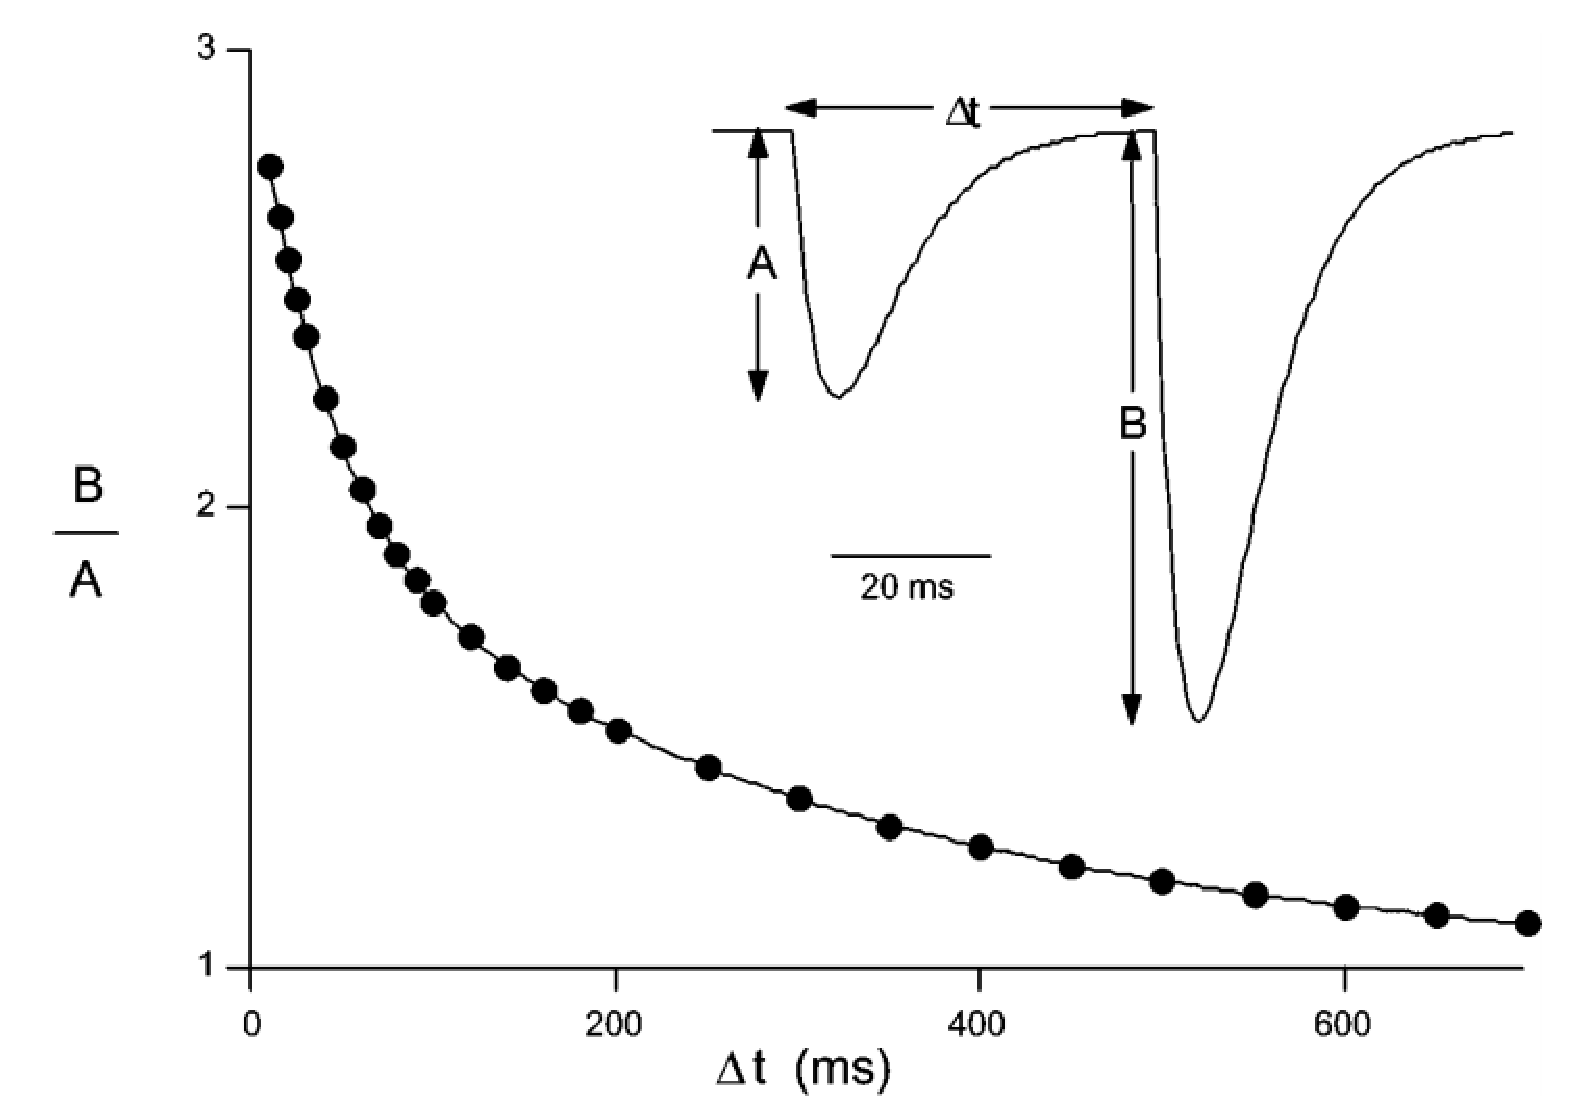
\includegraphics[height=4cm,
    angle=0]{./images/PairPulseFacilitation.eps}}
\caption{Pair-Pulse Facilitation (PPF): the time interval $\Delta t$ determines
the gain in response at the second AP (B) over the first AP (A).
Check eq.\ref{eq:pair-pulse-plasticity} for how to calculate the ratio.
The amplitude of facilitation (solid line below) can be approximated by a double
exponential decay of the form $1 + C_1 \exp(-t/\tau_1) + C_2 \exp(-t/\tau_2)$}
\label{fig:PairPulseFacilitation}
%http://mhs3.mp.kanazawa-u.ac.jp/eng/staff/rihabiri/shosaku.html
\end{figure}

\begin{mdframed}

{\bf paired pulse facilitation} (PPF):  A form of STF in which there is
only two successive presynaptic AP involved. \textcolor{red}{This occurs when
the first spike has a low release probability}; otherwise depression will
occur, Fig.\ref{fig:short-term-plasticity}(A).

\textcolor{red}{residual $\Ca$ hypothesis} (proposed by Katz and Miledi, 1954):
If the presynaptic cell has a low release probability of neurotransmitters, then
the first spike will cause a small postsynaptic response (read
Sect.\ref{sec:chemical_synapse} on how neurotransmitter depolarize postsynaptic
side), but the build-up of calcium in the presynaptic terminal (10-100$\muM$ at
the release sites  due to the openning of presynaptic terminal $V_m$-gated $\Ca$
channels) enables vesicle fusion - $\Ca$ binds to multiple low-affinity sites on
synaptotagamin to trigger vesicle fusion \citep{regehr2012}).

Depending on the time interval to the second AP.
An absolute refractory period was reached when intervals were about 10 ms apart.
When increasing the depolarizing stimulus from 1-2 ms, neurotransmitter release
greatly increased due to accumulation of active Ca2+.
Facilitation is greatest when the impulses are closest together because Ca2+
conductance would not return to baseline prior to the second stimulus.
In  calyx of Held synapse (Sect.\ref{sec:synapse-calyx-of-Held}), $\Ca$ binds to
neuronal $\Ca$ sensor 1 (NCS1) to perform facilitation \citep{gomez2001}.
\url{https://en.wikipedia.org/wiki/Neural_facilitation}

The increased release of neurotransmitters on the second AP leads to a greater
postsynaptic response, \textcolor{red}{upto about 5x postsynaptic
potential (PSP) of the first}, depending on the $\Delta t$ time interval,
Fig.\ref{fig:PairPulseFacilitation}.
\footnote{\url{https://wiki.brown.edu/confluence/display/BN0193S04/paired+pulse+facilitation+index}}

The high level of presynaptic calcium is short-lived. Once the VDCC closed, the
spatial gradient collapse as $\Ca$ diffuses and bind to $\Ca$-binding proteins,
such as calmodulin, calcium-binding protein-1, and
visinin-like protein-2.

The proteins, with rapid kinetics, can be  effective at intercepting
calcium before it can reach release sites. This leaves a smaller amount of
$\Ca$, called residual calcium (100s of nM) and long-lived (100s of
millisecond) - note the resting level is about 100nM. \textcolor{red}{This
residual calcium plays an important role in short-term plasticity.}

\end{mdframed}


% Synaptic enhancement builds and decays with a time course approximated by an
% exponential of $\sim 100$ milliseconds time scale is referred to as {\bf
% facilitation}.

Synaptic facilitation is explained by the build up of $\Ca$ in the presynaptic
terminal (i.e. the entry of $\Ca$ via $V_m$-dependent $\Ca$ channels in the
presynaptic terminal occurs within a millisecond or two after AP invades, but
the time for bringing $\Ca$ back to the resting level is much slow, and thus
$\Ca$ can easily build up at multiple APs are close together in time).
These calcium binds to a protein called {\bf synaptotagmin} located on the
membrane of the synaptic vesicles. This protein then interacts with the
trafficking proteins called SNARE to induce vesicle fusion with the presynaptic
membrane. This calcium-protein interactions then produce a change in vesicle
exocytosis (i.e. an energy-consuming process directing the
neurotransmitter-contained vesicle out of the cell membrane), i.e. allows more
neurotransmitter to be released.

\begin{verbatim}
successive presynaptic AP ---> build-up presynaptic [Ca]
      ---> [Ca] affect level of neurotransmitter released 
\end{verbatim}

Depending the types of presynaptic neurons, there can be different types of
neurotransmitter releases (Sect.\ref{sec:neurotransmitter}), which will affects
the post-synaptic side differently (Sect.\ref{sec:synapse-activation}).

% Another potential factor is caused by the increased transmitter release
% produced by two or more action potential invading the presynaptic terminal in close
% succession. 
In some synapses, the vesicles are grouped into fast-release pool
and slowly-release pool. So, facilitation in these synapses is divided into a
rapid phase lasting 10s of milliseconds (F1), and a slower phase lasting 100s of
milliseconds (F2), Fig.\ref{fig:PairPulseFacilitation}.
At many synapses the distinction between F1 and F2 is not clear, and the
duration of facilitation is well approximated by a single exponential fit
  
However, prolonged stimulation is usually accompanied by depression
(Sect.\ref{sec:short-term_depression}). \textcolor{red}{Potentiation is often
only observed after a tetanus, following recovery from depression}, 
Fig.\ref{fig:short-term-plasticity}(D).

\begin{figure}[htbp]
  \centerline{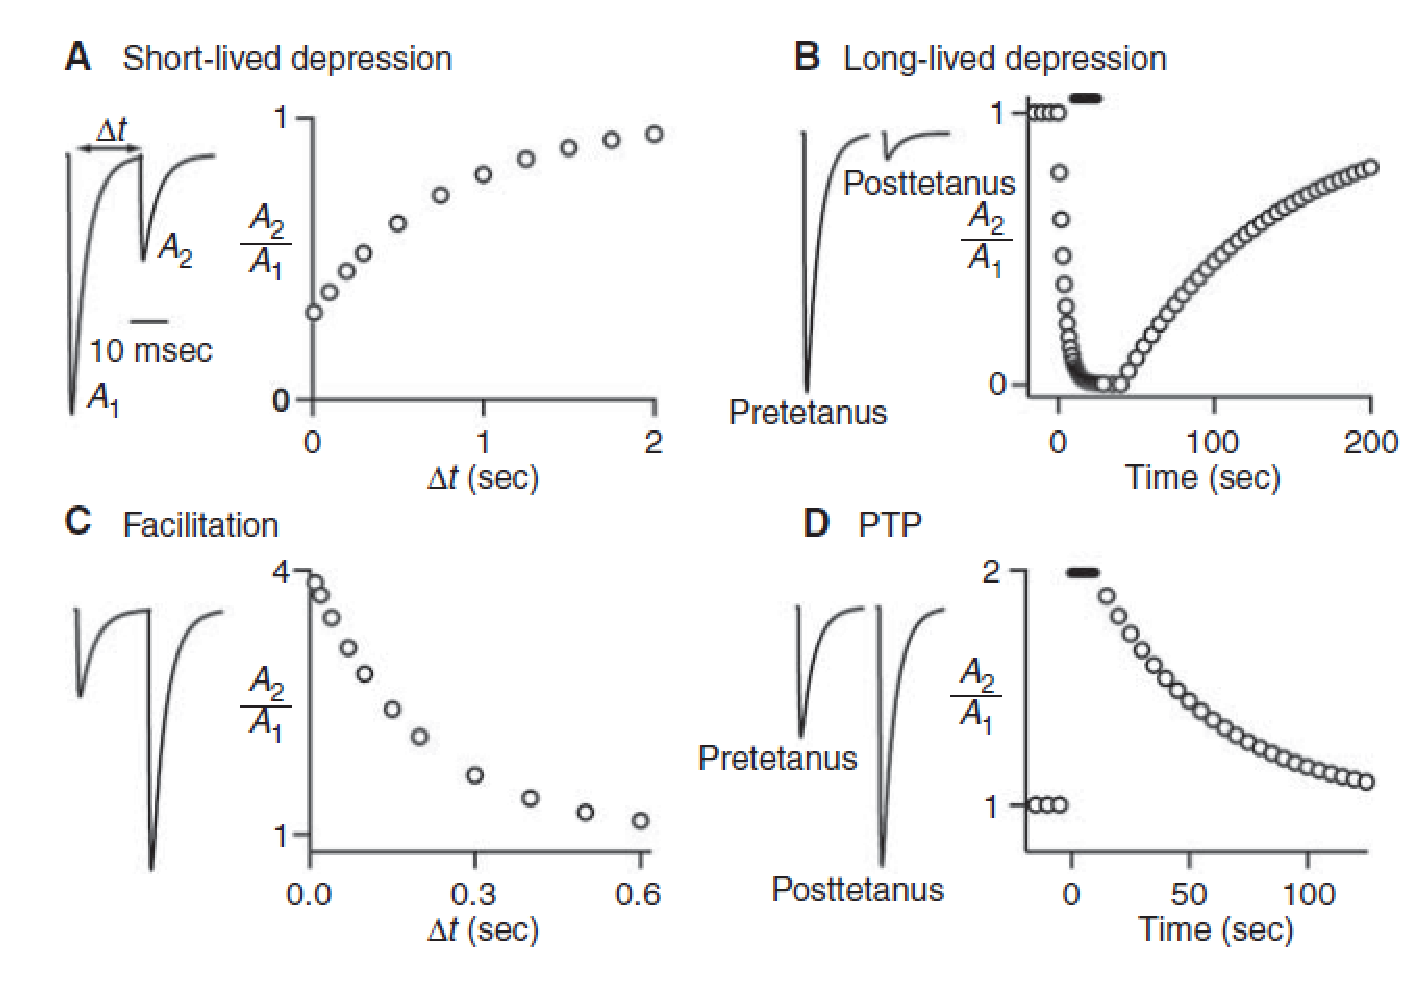
\includegraphics[height=6cm]{./images/short-term-plasticity.eps}}
  \caption{(A) short-lived depression; (B)
  long-lived depression; (C) short-term
  facilitation; (D) PTP \citep{regehr2012}}\label{fig:short-term-plasticity}
\end{figure}

The presence of high-affinity calcium buffers in presynaptic boutons can also
produce facilitation. If present at sufficiently high concentrations, they can
bind calcium after it enters through voltage-gated calcium channels and before
it reaches release sites.

In this way calcium-binding proteins can reduce $\Ca$ local at the release site.
Fast calcium buffers such as calbindin (Sect.\ref{sec:calbindin}) can reduce the
initial probability of release in the same way that introducing the fast
buffer BAPTA into the presynaptic terminal lowers the initial probability of
release. If calcium levels in the presynaptic bouton are sufficiently high, then
after the first stimulus a high-affinity calciumbinding protein will be
primarily bound to calcium.
As a result, more of the calcium that enters the bouton in response to a
subsequent action potential will reach the release site.

\subsection{** short-term potentiation (STP)}
\label{sec:short-term-potentiation}

{\bf short-term potentitation}  (STP): which is in the form of {\bf
Augmentation} (Sect.\ref{sec:STP-augmentation}) / {\bf Post-tetanic potentiation
(PTP)} (Sect.\ref{sec:STP-PTP}), i.e. a short-term transient increases in
synaptic strength when after the end of a trains of stimulus (2 or more APs
arrives within a few  milliseconds).

  At the end of a high-frequency burst of presynaptic action potentials
  (colloquially referred to as a ``tetanus") at 10 Hz - 200 Hz applied for 0.2 sec to 5 sec,
  the synapse response to the next single AP with an enhancement in mEPSP or
  EPSC. 

\subsection{+++ augmentation} 
\label{sec:STP-augmentation}
 
{\bf Augmentation}: A form of STP in which potentiations shorter than a
  minute. The growth and decay with a time constant of $\sim 5-10$ second.
  In some synapses, augmentation and PTP components are not easily separable,
 and they are often lumped together and referred to as PTP.

\subsection{+++ short-term post-tetanic potentiation (PTP)}
\label{sec:STP-PTP}

  {\bf post-tetanic potentiation} (PTP): A form of STP that
  occurs with a delay (after the end of the train of stimulus),
  Fig.\ref{fig:STplasticity}, and last for 30 second to several minutes
  \citep{huges1958}. It was first recognized in the frog neuromuscular
  junction.
    
  \textcolor{red}{What is the mechanism of PTP?}: An increase in release
  probability (Pr), or an increase in readily-released vesicles, or an increase
  in both? $\Ca$ can play either direct or indirect role (review:
  \citep{zucker2002})
  \begin{itemize}
    \item 
  PTP is thought to arise from calcium-dependent processes that make
  more synaptic vesicles available for transmitter release due to the persistent
  presynaptic $\Ca$ level even the train of stimulus has ended. This was
  suggested due to a slow efflux of $\Ca$ from accumulated mitochondrial $\Ca$
  \citep{tang1997}. 
  
    \item Another paper by Lee and coworkers suggested the indirect role of
    $\Ca$ via $\Ca$-binding calmodulin (CaM) found in calyx of Held (large synapse in the
  auditory CNS) (review: \citep{balakrishnan2010}).
  
  In the calyx, CaM mediates the rapid recruitment of fast-releasing synaptic
  vesicles. Also, CaM can activate myosin lightchain kinase (MLCK) - regulate
  myosin II activity via phosphorylation. This will enable the myosin
  cross-bridge to bind to the actin filament and allow vesicle mobility.
  
    \item Another paper suggested the contribution of postsynaptic $\Ca$, along
    with peresynaptic $\Ca$, in PTP found in a subset of siphon sensory to motor
    neuron (SN-MN) synapse in Aplysia\citep{schaffhausen2001}. However, this is not
    found in other types of synapses.
    
    Blocking the rise in postsynaptic $\Ca$ via either the strong postsynaptic
    hyperpolarization or injection of $\Ca$ chelator BAPTA during presynaptic
    tetanus reduces the amount of PTP. These observations suggest that at least
    some synapses may require an influx of postsynaptic $\Ca$ for the induction of PTP.
  \end{itemize}
  \url{http://standoutpublishing.com/g/post-tetanic-potentiation.html}

\subsection{** short-term depression (STD)}

{\bf short-term depression (STD)}: Short-term depression
suppresses neurotransmitter release for hundreds of milliseconds to tens of
seconds.


  {\bf Pair-pulse depression} is hard to observe with pair-pulse protocol with
  initial low probability of release, but at high $[\Ca]_e$, the depression
  becomes more prominent,
  Fig.\ref{fig:Role_initial-Pr-in-synaptic-plasticity} (\textcolor{blue}{blue}
  trace).

  At some synapses, repeated stimulus lead to synaptic enhancement; while
  at others the result is a decrease in synaptic strength and depression
  prevails. Synaptic depression dominates enhancement at many synapses.
  
\textcolor{red}{ The mechanism leading to STD can be} 
  \begin{enumerate}
    \item depletion model (explained by depletion of available neurotransmitter
    for release due to depletion of RRP). 
%     If more vesicles fuse in response to the initial stimulus,
%     there is more depletion of the RRP and fewer vesicles are released by the
%     second stimulus.
    
    If the first stimulus trigger the release of a large fraction of RRP, there
    is more depletion of the RRP and fewer vesicles are released by the second
    stimulus. Even though it has long been assumed that AP could evoke the
    release of at most a single vesicle at an individual active zone (Redman
    1990; Korn et al. 1994), several newer evidences suggested that at many
    synapses multivesicular release occurs.
       
The depletion model predicts a negative correlation between EPSC2 and EPSC1 for
two closely spaced stimuli. This has been observed in neuromuscular junction
(Elmqvist and Quastel 1965), hair cell synapses (Furukawa et al. 1978), the
calyx of Held (Scheuss et al. 2002), thalamocortical synapses (Ran et al. 2009),
cortical connections (Thomson et al. 1993), and hippocampal synapses (Debanne et
al. 1996). 


\textcolor{red}{However, this simple depletion model is not good enough to
explain the mechanism at some synapses, as the extent of depression does not
appear to depend} on the magnitude of release evoked by the first stimulus (Thomson and Bannister 1999;
Kraushaar and Jonas 2000; Chen et al. 2004) or the size of the RRP (Sullivan
2007), and an inverse correlation has not been seen at synapses onto Mauthner
cells (Waldeck et al. 2000) and at hippocampal synapses (Chen et al. 2004).

    \item inactivation of release sites: this assumes that fusion of a vesicle
    at an active zone can inhibit subsequent fusion of available vesicles for
    several seconds.
     
    However, site inactivation does not appear to occur at many types of
    synapses, which are capable of releasing tens of vesicles per active zone each second
    (Saviane and Silver 2006; Crowley et al. 2007).

% blocking endocytosis () leads to more pronounced depression during trains
    \item depression followed tetanic stimulation,
    Fig.\ref{fig:STplasticity}(B):
    The stimulation is sufficiently prolonged to deplete the recycling pool
    (RP), and is at high enough frequency such that replenishment
from the NRP or recycling via endocytosis would be unable to keep up with
vesicle loss during tetanic stimulation.

    \item inactivation of VDCC $\Ca$ channels:
    
    \item other mechanisms of depressions:
    (1) alteration in the firing threshold for somatic or extracellular
    activation that involves the Na/K-ATPase (Munoz-Cuevas et al. 2004), (2)
    failure of an AP to invade the axonal branches (in cultured hippocampal
    cells, i.e. explain the fact that the depression observed is just the
    side-effect of the experiment and is not present in the intact cell)
        
    \item desensitization of postsynaptic receptors: 
    
Depression can also arise from feedback activation of presynaptic receptors and
from postsynaptic processes such as receptor desensitization.
Thus, prolonged stimulation can lead to facilitation first and then depression.

\end{enumerate}
Following sustained stimulation the time constant of recovery
shifts from seconds to tens of seconds. This reflects (1) the slow replenishment
of the RRP from RP, (2) decrease in $\Ca$ entry, (3) decrease in probability of
release.

\textcolor{red}{Regulation of depression}:
\begin{enumerate}
  \item knockout of Bassoon, a large presynaptic
protein present at the active zone, leads to
enhanced synaptic depression

  \item synapsins: 
  the elimination of synapsins decreases
the number of vesicles in presynaptic
boutons and leads to more pronounced depression
during sustained moderate-frequency
stimulation (Rosahl et al. 1995; Gitler et al.
2008).
   
\end{enumerate}

\textcolor{red}{Recovery from depression}:
\begin{enumerate}
  \item    Elevations of presynaptic calcium can greatly accelerate recovery from
   depression, i.e. accelerating replenishment of the RRP. \textcolor{red}{This
   acceleration is prevented by inhibiting calmodulin; yet the
   downstream of $\Ca$-bind calmodulin (CaM) target remains unclear.}
  
  In calyx of Held synapse, activation of Gi/o coupled
receptors (Sect.\ref{sec:G-protein-coupled-receptor}) lowers presynaptic cAMP,
which prevents calcium-dependent recovery from depression (Sakaba and Neher
2003).
   
   \label{sec:alpha-synuclein-modify-vesicle}
   \item $\alpha$-synuclein (Cabin et al. 2002) -
   Sect.\ref{sec:alpha-synuclein}: reduces the size of the pool of nondocked
   vesicles by $\approx$  40\% and reduces the extent of depression during
   sustained stimulation by $\approx 30$\% .

   \item rabphilin: a protein that interacts with the GTP-binding proteins Rab3A
   to -D, contains two C2 domains that bind calcium, and binds to the SNARE
   protein SNAP-25:

Removing of rabphilin accelerates recovery from depression
following 20-Hz, 60-sec stimulation (fast
component of recovery with $\tau = 4$ sec becomes
prominent, whereas slow component with $\tau =$
60 sec dominates in control conditions (Deak et al., 2006).

\end{enumerate}

At present the mechanism by which these molecules regulate recovery from
depression is not known.

% NOTE: If there is only two successive presynaptic potential and cause short-term
% depression, it is called paired pulse depression (PPD).
% If the presynaptic cell has high release probability, then the first pulse will
% deplete the available transmitter, and the second pulse will cause less
% transmitter to be release, leading to a low PPF or even PPD (depression)


At the calyx of Held synapse, short-term depression is largely a result of
decreased calcium entry for activation frequencies of $< 30$ Hz and primarily a
result of depletion at frequencies $> 100$ Hz; at intermediate frequencies both
mechanisms contribute (Xu and Wu 2005).

% \subsubsection{STF (STP)}
% 
% As the AP returning to normal is slower than the diffusion of $\Ca$ into the
% terminal that occurs when AP trigger $V_m$-gated $\Ca$ channels. Thus, $\Ca$
% build-up in the pre-synpatic terminals.
% The excess $\Ca$+ may bind to sites on synaptotagmin
% (Sect.\ref{sec:mechanism_neurotransmitter-release}), allowing more presynaptic
% vesicles to fuse with the membrane when the next AP arrives.
% 
% Facillitation increases the amount of neurotransmitter released with each
% subsequent AP, and thus increase the postsynaptic potential
% (Sect.\ref{sec:postsynaptic_potential}) \textcolor{red}{This is presynaptic
% mechanism}.
% 
% In STF, the EPSP evoked by an impulse are increased when that impulse is closely
% follows a prior impulse. This is explained at the presynaptic, where an
% increased presynaptic [$\Ca$] leading to a greater release of
% neurotransmitter-containing synaptic vesicles (Sect.\ref{sec:Acetylcholine}).
% The details is given below
% \begin{itemize}
%   \item when an AP invades the presynaptic membrane, the ion channels there open
%   and Ca2+ enters
% \end{itemize}
% 
% 
% \subsubsection{STD}
% 
% With depression, the amount of neurotransmitter released per AP decreases with
% each subsequent AP. In STD, the decrease lasts a few seconds.
% This is probably due to depletion of vesicles ready to fuse with the membrane.
% 
% \subsubsection{Augmentation}
% 
% Augmentation increases the ability of $\Ca$ to cause vesicles to bind.
% \textcolor{red}{Mechanism is unclear}. Augmentation lasts a few seconds and is
% often obscured by depression.
% 
% \subsubsection{PTP}
% 
% Post-tetanic potentiation (PTP) occurs after several seconds of high-frequency
% stimulation (tetanus). PTP is due to increased neurotransmitter release
% resulting from buildup of Ca2+ in the presynaptic terminal. It lasts up to 1-2
% minutes. This is indeed an extreme case of short-term potentiation.
% This, again, is a presynaptic mechanism.
% 
% Exact mechanism is unknown, possibly due to activation of protein kinases that
% phosphorylate synapsin. 
% 
% \url{http://132.236.112.18/wytt/3/notes3w.pdf}

\subsection{+++ STDP: STD}

STDP-STD: At hippocampal synapses, PLC$\beta$ is an efficient coinciedence
detector triggering retrograde endocannabinoids signaling to mediate short-term
depression (Sect.\ref{sec:cannabinoid-receptors}) \citep{hashimotodani2005}. 


\subsection{- Long-term plasticity: LTD + LTP}
\label{sec:LTplasticity}
\label{sec:mechanism-long-term-plasticity}
\label{sec:long-term_potentiation}
\label{sec:long-term_depression}
\label{sec:LTD}

Short-term plasticity is not considered important in forming memory; instead
long-term plascitity is the one leading to memory formation.
%Also, in short-term plasticity, the stimulus comes from the presynaptic side.
Even though long-term plasticity can link to short-term plasticity, we mainly
focus on long-term plasticity. 

\textcolor{red}{Two forms of long-term synaptic plasticity}: Long-term
plasticity is the condition that causes a significant change in the synaptic plasticity which lasts hours or years in the excitatory or inhibitory
synapse. {\bf Long-term depression} (LTD) and {\bf long-term potentiation} (LTP)
are two opposite forms of long-term plasticity.
Early studies focused on LTP (Sect.\ref{sec:LTP}) as LTP is widely considered
one of the major cellular mechanisms that underlies learning
(Sect.\ref{sec:learning}) and memory (Sect.\ref{sec:memory_brain}).
Then, LTD was then proved to exist as a mechanism of the neuron to provide a
counterpart to LTP. Most data so far come from hippocampal slice preparations,
where it is possible to examine a few synapses in cell culture.

\textcolor{red}{Bidirectional synaptic plasticity}: Early evidences in striatum
suggest a synapse (from one neuron type) can only either switch to LTP or LTD
but not both, i.e. mutually exclusive (Calabresi et al., 1996; Mahon et al.,
2004). If this is the case, a resetting of transmission efficacy at these
synapses would be impossible, a situation hardly consistent with striatal
functions in sensorimotor learning. Recent evidences suggested that a synapse
once in LTP can switch to LTD, or once in LTD can switch to LTP, depending on
the proper situations, i.e. the bidirectional synaptic plasticity via STDP
protocol (Sect.\ref{sec:STDP}).

The molecular mechanisms of LTP/LTD can be divided into two phases: {\bf
induction}, triggering the potentiation or depression; and {\bf maintenance},
sustaining the potentiation/depression over time. With long-term plasticity,
\textcolor{red}{the challenging questions are}
\begin{enumerate}
  \item for a given neuron connection, what is the source
  of changes (in synaptic efficacy)? (Sect.\ref{sec:source-synaptic-plasticity})

  Early work in the sea snail Aplysia identified a number of kinases that show
  this type of persistent activity following synaptic stimulation, including PKA
  (cAMP-dependent protein kinase A), CaMKII (Ca2+/calmodulin-dependent protein
  kinase II), and PKC (protein kinase C) ( Schwartz and Greenberg, 1987 and
  Schwartz, 1993). Blocking these proteins, however, affected the development of
  {\it intermediate-term facilitation}, rather than the maintenance of long-term
  potentiation ( Sutton and Carew, 2000).


  \item and what help to maintain this changes (i.e. even without the source of
  this change?   (Sect.\ref{sec:mechanism-long-term-plasticity}). Understanding
maintenance, however, is critical for testing the hypothesis that LTP sustains
memory storage in the brain.

 
  From that we can learn under what condition this change is sustained or
  abolished, or the survival time for the plasticity or the level of change in
  synaptic efficacy is not the same.

LTP in the CA1 hippocampal region and dentate gyrus is known to be induced
postsynaptically.  Only a single molecule has been found both necessary and sufficient for
  maintaining LTP--the brain-specific, atypical PKC isoform, protein kinase
  Mzeta (PKMzeta - Sect.\ref{sec:PKMzeta}) \citep{sacktor2008}.
  However, the true role of PKMzeta as maintaining memory or just a
  restabilization mechanism is still debated (review: \citep{kawapi2014})


   \item   the causal link between LTP and behavioral learning
\end{enumerate}

\begin{mdframed}
LTP and LTD are known in hippocampus (Sect.\ref{sec:hippocampus}), cortex
(Sect.\ref{sec:cerebral_cortex}), amygdala (Sect.\ref{sec:amygdala}), and
cerebellum (Sect.\ref{sec:cerebellum}) (at least).
\end{mdframed}

\subsection{** LTP}
\label{sec:LTP}
\label{sec:LTP_depend-NMDAR}
\label{sec:BDNF-mediate-LTP}


\textcolor{red}{\bf Where is LTP}: LTP was first found in synpase connecting
neurons in EC to dentate gyrus (i.e. perforant pathway -
Sect.\ref{sec:perforant-pathway}) in rabbit hippocampal formation
(Sect.\ref{sec:hippocampal_formation}) in 1966 by Lomo \citep{lomo1966}.
LTP has been observed in a variety of other neural structures, including the
cerebral cortex, cerebellum, amygdala \citep{malenka2004}.
However, the mechanism leading to LTP can be different in different brain
regions. In other words, different areas in the brain may exhibit different
forms of LTP. To elucidate the different underlying cellular mechanism leading
to LTP, different induction protocols have been used:

\begin{enumerate}
  \item {\bf age of organism when LTP is observed}: 
  mechanism of LTP in immature hippocampus is different from that in mature
  hippocampus \citep{yasuda2003}.

  \item {\bf signaling pathways involved}:
  \begin{enumerate}

    \item depending on NMDAR:
    NMDAR-dependent LTP also exhibits at least two phases, denoted early and
    late LTP.
    % LTP in the Schaffer collateral pathway of the hippocampus.
     
The below properties of NMDAR-dependent LTP
\begin{itemize}
  \item {\it specific}: tetanic stimuli at one synapse strengthens only that
  synapse (exceptions below).
  
%  \item {\it cooperativity}:  
  \item \textcolor{red}{cooperativity} = (even though 'weak' stimulus is
  insufficient to induce LTP), many weak stimulus from many pathways that
  converve on a single patch of postsynaptic membrane can induce LTP. 

  \item \textcolor{red}{associativity} = when a 'weak' input is insufficient
  to induce LTP, the simultaneous 'strong' stimulation of another pathway can
  induce LTP at both pathways.
  
Cooperative-induced LTP is a special case of associative LTP:  both originate from
the requirement in the synchrony of inputs for postsynaptic activation
\citep{teyler1987}.
  
  \item {\it state-dependent}:  if the postsynaptic cell is depolarized, it can
  get LTP from a stimulus that ordinarily would not evoke LTP when it is not
  depolarized.

%   \item {\it associative} (from 2 synapses): Weak stimulation of one pathway
% during strong stimulation of another pathway can strengthen both synapses.

This is in part due to state dependence - the weakly stimulated synapse is
depolarized by EPSPs arriving from the strongly stimulated synapse.
 
   \item {\it persistence} (the enhancement in synaptic efficacy lasts from
   several minutes to many months):    This is the very first property, i.e.
   it is this persistence that  separates LTP from other forms of synaptic
   plasticity.
\end{itemize}


   \item \textcolor{red}{NMDAR-independent LTP} has also been observed:

\begin{itemize}
  \item mGluR-dependent LTP (which uses G-protein signalling pathway):  
  
  \item cAMP-dependent presynaptic forms of LTP:
  activation of dopamine receptors may enhance LTP through the cAMP/PKA
  signaling pathway.  
 \end{itemize}
 LTP in  the mossy fiber pathway is NMDA receptor-independent.

 \end{enumerate}
Overall, LTP is an increase in the postsynaptic sensitivity to glutamate.
However, LTP may also increase presynaptic glutamate release due to a retrograde
signal (Sect.\ref{sec:glutamate_receptor}). The second mechanism, nevertheless,
is still controversal. 

\end{enumerate}

% TODO:
TODO: Put the below into NMDAR-dependent or NMDAR-independent LTP

\begin{enumerate}
  \item PKA - Sect.\ref{sec:PKA-function}
\end{enumerate}

\subsection{+++ early phase LTP}

{\bf early phase} LTP (LTP1, E-LTP): lasts for
  only 1-3 h and does not require protein synthesis (i.e. AMPAR in the postsynaptic membrane), but cause
  phosphorylation of AMPAR, i.e. it increase sensitivity of the synapse,
  (resulting in increase $P_o$).

LTP is evoked by high-frequency activity (tetanus), during which EPSP generated
by AMPAR accumulate and build up over time can cause depolarization enough to
remove $\Mg$ block of NMDA receptors (Sect.\ref{sec:NMDA}).

As NMDAR activation, it brought $[\Ca]$postsynaptic increase which bind to
calmodulin, and then $\Ca$-bound calmodulin (CaM) activate CaMKII
(Sect.\ref{sec:CaMKII}). Activated CaMKII phosphorylates existing AMPAR
on GluA1 AMPA subunit at site Ser831 (increase single channel conductance)
and/or Ser845 on GluR1 subunit of AMPAR \citep{kristensen2011}

  The delivery of AMPA receptors to the synapse during E-LTP is independent of
  protein synthesis. This is achieved by having a nonsynaptic pool of AMPA
  receptors adjacent to the postsynaptic membrane.
  When the appropriate LTP-inducing stimulus arrives, nonsynaptic AMPA receptors
  are rapidly trafficked into the postsynaptic membrane under the influence of
  protein kinases.
  %Malinow R (2003). "AMPA receptor trafficking and long-term potentiation".
  % Philos Trans R Soc Lond B Biol Sci 358 (1432): 707-14

  Persistent CaMKII activity in the postsynaptic cell during E-LTP may lead to
  the synthesis of a "retrograde messenger" - that can  travel across the
  synaptic cleft from the postsynaptic to the
   presynaptic cell, leading to a chain of events that facilitate the
   presynaptic response to subsequent stimuli. Such events may include an
   increase in neurotransmitter vesicle number, probability of vesicle release,
   or both. In addition, retrograde messenger may also play a role in the
   expression of late LTP.

After tetanus, post-synaptic potential (PSP -
Sect.\ref{sec:postsynaptic_potential}) amplitude is increased and sustained at a
level above the baseline response for 1-3 HOURS.

\subsection{+++ late phase LTP2}

{\bf late phase } (LTP2): (the natural extension of early LTP, to occur
  after 1 hours or so of continuous stimulation):   lasts for at least a day and
  requires only protein synthesis (mRNA translation)
  
  
  The first mode of CaMKII activation is phosphorylate synaptic-associated
  protein 97(SAP97).
  SAP-97 and Myosin-VI, a motor protein, are bound as a complex to the
  C-terminus of AMPARs. Phosphorylated SAP-97 then move to perisynaptic
  membrane.
  
  The second mode of CaMKII activation is through MAPK pathway.
  CaMKII activates the Ras proteins, which go on to activate p42/44 MAPK (or
  ERK2/ERK1) (Sect.\ref{sec:MAPK}), which drives AMPAR insertion directly into
  the perisynaptic membrane \citep{zhu2002}.
  LTP can involve structural changes to the dendritic spine, i.e. increase
  volume to accommodate more AMPAR or split one into two separate dendritic
  spines.
    
  The latter may be brought about in part by the enhanced synthesis of AMPA
  receptors during L-LTP.
% The persistent activation of protein kinase, e.g. MAPK , during LTP1.
  Once AMPA receptors are transported to the perisynaptic region through PKA or
  SAP97 phosphorylation, receptors are then trafficked to the postsynaptic
  density (PSD).
  However, this process of trafficking to the PSD still remains controversial.
  \begin{itemize}
    \item lateral movement of AMPA receptors from perisynpatic sites directly to
    the PSD. \citep{borgdorff2002} \ref{sec:AMPAR}
    %Borgdorff AJ, Choquet D (June 2002). "Regulation of AMPA receptor lateral
    % movements". Nature 417 (6889): 649-53. 

    \item  exocytosis of intracellular vesicles is responsible for AMPA
    trafficking to the PSD directly. \citep{park2004re}
    %Park M, Penick EC, Edwards JG, Kauer JA, Ehlers MD (September 2004).
    % "Recycling endosomes supply AMPA receptors for LTP". Science 305 (5692): 1972-5.
  \end{itemize}
  Recent evidence suggests that both of these processes are happening after an
  LTP stimulus; however, only the lateral movement of AMPA receptors from the
  perisynaptic region enhances the number of AMPA receptors at the PSD
  \citep{makino2009}.
%Makino H, Malinow R (November 2009). "AMPA receptor incorporation into synapses
% during LTP: the role of lateral movement and exocytosis". Neuron 64 (3): 381-90
  
  In addition to influencing synaptic localization, SAP97 has also been found to
  influence AMPA receptor conductance in response to glutamate.
  Myosin proteins are calcium sensitive motor proteins that have also been found
  to be essential for AMPA receptor trafficking. 
  CACNG2 (Stargazin) is one such protein and is found to bind AMPA receptors in
  the perisynpatic and postsynaptic regions, yet its role in AMPAR tracficking
  is unknown. 
  However, stargazin is essential for immobilizing AMPA receptors in the PSD by
  interacting with PSD-95.
  \url{https://en.wikipedia.org/wiki/AMPA_receptor}

  NMDAR activation in CA1 subfield of hippocampus slide results in superoxide
  production. The $\alpha$, $\beta$II, $\varepsilon$ and $\zeta$ isotypes of PKC
  are autonomously activated by reactive oxygen species by thiol oxidation and
  release of zinc from cysteine-rich regions of PKCs. The persistent activation
  of these PKC (Sect.\ref{sec:PKC}) is important for maintenance of LTP
  response, i.e. PKMzeta. The increased level of PKMzeta then enhances synaptic
  transmission by doubling the number of postsynaptic AMPA receptors (AMPAR)
  through GluR2 subunit-mediated trafficking of the receptors to the synapse
  \citep{sacktor2008}

An important regulatory pathway for PKC activation is the liberation of c-FAs
from membrane phospholipids by PLA2. In LTP, activation of this pathway may
stabilize PKC in an activated state, and thus contribute to maintenance of the
potentiated response
  
  Recent research has shown that the induction of L-LTP can depend on coincident
  molecular events, namely PKA activation and calcium influx, that converge on
  CRTC1 (TORC1), a potent transcriptional coactivator for cAMP response element
  binding protein (CREB)
  %Kovacs KA, Steullet P, Steinmann M, Do KQ, Magistretti PJ, Halfon O,
  % Cardinaux JR (2007). "TORC1 is a calcium- and cAMP-sensitive coincidence detector involved in hippocampal long-term synaptic plasticity.". PNAS 104 (11): 4700-5.
  
  Similar to retrograde messenger discussed for early-LTP (retrograde
  signaling), Late LTP is also associated with the presynaptic synthesis of synaptotagmin and an increase in
  synaptic vesicle number, suggesting that L-LTP induces protein synthesis not
  only in postsynaptic cells, but in presynaptic cells as well.
  %Lynch M (2004). "Long-term potentiation and memory". Physiol Rev 84 (1):
  % 87-136.
  
  Retrograde signaling is currently a contentious subject as some investigators
  do not believe the presynaptic cell contributes at all to the expression of LTP
  \citep{malenka2004}.
Early thoughts focused on nitric oxide, while most recent evidence points to
cell adhesion proteins.

\subsection{+++ late phase LTP3}

{\bf late phase} (LTP3): (to occur after 1
  hours or so of continuous stimulation):   lasts for at least a day and
  requires both (1) mRNA translation (protein synthesis) and new gene
  transcription in the postsynaptic neuron.
  
  ERK may phosphorylate a number of cytoplasmic and nuclear molecules.
  These cytoplasmic and nuclear molecules may include transcription factors such
   as CREB
   %Sweatt J (1999). "Toward a molecular explanation for long-term
   % potentiation". Learn Mem 6 (5): 399-416.
   ERK-mediated changes in transcription factors trigger the synthesis of
   proteins that underline maintenance of late-LTP, such as MPKzeta
   (Sect.\ref{sec:PKMzeta})
  
  This results in an increase in AMPAR production and trafficking from internal
  stores to the postsynaptic membrane and increase the size of synaptic
  connection and dendrites may add new spines (new synapses, at least one more)
  \citep{toni1999}.
  
  Maintenance of LTP over time requires AMPAR protein synthesis which
  requires continuous stimulation (at least in rat because LTP declines if
  synthesis is inhibited).

\subsection{Activity-dependent synaptic plasticity}
\label{sec:activity-dependent-synaptic-plasticity}


When we say about {\bf activity}, it means that the neuron (can be presynaptic
side or postsynaptic side or both) has to generate the spike (or action potential) to
induce the change.

The change in synaptic plasticity as a result of tetanus stimulation as in the
case of Hebbian plasticity (Sect.\ref{sec:Hebbian-plasticity}) is aka
{\bf activity-dependent synaptic plasticity} (or use-dependent synaptic
plasticity).


\subsection{ * Hebbian's postulate}

Hebb (1949) then proposed a physiological association principle -  a mechanism
for this to happen (Sect.\ref{sec:Hebbian-synapse}), {\it but only focus on the
aspect of increase synaptic effiency via co-activiation and for excitatory} (see below).

Hebb's postulate (1949): {\it When an axon of cell A ({\bf presynaptic}) is near
enough to excite cell B ({\bf postsynaptic}) and cell A repeatedly or
persistently takes part in firing, some growth process or metabolic change
takes place in one or both cells such that A's efficiency as one of the cells
firing B (i.e. the excitability of B), is increased.
}. 

In Hebb's original postulate, cell A fires before cell B.
Such temporal specificity of activity-induced synaptic modification may be
relevant for physiological functions, such as learning and memory, which are
known to be temporally specific.

\subsection{ * Hebbian theory}
\label{sec:Hebbian-theory}

The classic Hebbian's postulate requires only pre-synaptic firing, and it
increases the synaptic efficacy.

Indeed, the modification can be the result of 
\begin{itemize}
  \item only post-synaptic firing
  \item coincidence of presynaptic and postsynaptic firing

A more popular version of this rule - postulated by neurobiologist Carla
Shatz: {\it neurons that fire together wire together}.
\end{itemize}

It was one possible way to reinforce functional coupling between co-active
cells, leading to forming an assembly. Similar hypotheses were developed at a
higher hierarchical level of organization that allowed linkaged between
cognitive events and their recall in the form of a temporally organized series
of activations of assemblies.

The formulation of Hebb's postulate requires
\begin{itemize}
  \item temporal specificity (the core of Hebb's postulate): closely temporal
  coincidence of activation on presynaptic neuron A and postsynaptic neuron B
  
 
  \item spatial specificity:  
  
  Although not explicitly stated in Hebb's postulate,  it is generally assumed that
Hebbian synaptic modifications are synapse (or input) specific-only synapses
experiencing correlated activity become modified. Thus, \textcolor{red}{Hebbian
rule is regarded as a 'local' rule}, in which individual synapses are
independent of one another. For non-local synaptic modification, see
Sect.\ref{sec:non-local-synaptic-modification}.
\end{itemize}

\subsection{+ Hebbian learning}
\label{sec:Hebbian-learning}

Based on Hebbian theory (Sect.\ref{sec:Hebbian-theory}) which talks about the
\textcolor{red}{increase of presynaptic neuron's efficacy} of eliciting activity
in the postsynaptic neuron (i.e. increase the excitability of the postsynaptic
neuron), under the same correlated firing condition (i.e. the
neurons fire together wire together). 

Hebb's idea has been extended into various forms of correlation-based rules for
synaptic modification and successfully used in many learning networks and in the
analysis of activity-driven refinement of developing circuits.

Hebbian learning is defined a little bit different:
correlated activation in the pre- and postsynaptic neurons leading to the
\textcolor{red}{increase the strength} of the connection between the two
neurons. These two definitions (strengthening of connection vs. increased
efficiency) are compatible only when the presynaptic neuron is excitatory.
They are contradictory when increased connection strength (weight, efficacy)
corresponds to decreased efficiency in eliciting response, i.e. hyperpolarized
the postsynaptic membrane potential. This is called anti-Hebbian learning
(Sect.\ref{sec:anti-Hebbian-learning}).



% It provides a specific prediction:
% \textcolor{red}{after a period of induction, i.e. a maintained positive temporal
% correlation between pre- and postsynaptic activity}, i.e. pre-synaptic activiation from
% neuron A on neuron B at a given frequency continuously for a certain period of
% time, \textcolor{red}{will lead to an increase in the efficacy of synaptic
% transmission}. 

{\bf IMPORTANT}: Hebb, however, did not point out the decrease in synaptic
resistance comes from the presynaptic side {\it (e.g. more vesicles of
neurotransmitter released)}, or postsynaptic side {\it (e.g. receptors becomes
more likely to open upon neurotransmitter binding)} or both. Neither did he
describes the substrate responsible for the modification (metabolic change or
oriented growth???). Nowadays, we now that both of the options turned out to be
true.

\subsection{ -- classic Hebbian synapse: (long-term) synaptic enhancement -
LTP}
\label{sec:Hebbian-synapse}
\label{sec:Hebbian-plasticity}

Hebbian synapses refer to excitatory synapses whose under high-frequency
stimulus (strong tetanic stimulation), \textcolor{red}{LTP is induced }.
LTP is a phenomenon where high frequency stimulation of the presynaptic neuron
(during the induction phases) leads to a prolonged increase in synaptic
efficacy.

\begin{verbatim}
pre-stimulus phase:
     (stimulate a few synapses) - measure EPSP (baseline)
	 (not enough to trigger spike in postsynaptic neuron)

firing phase: strong presynaptic tetanic stimulation
 (that lead to spike in the postsynaptic neuron)
   15Hz for 15 seconds or
   100Hz for 3 seconds

measuring phase:
 (stimulate a few synapse at 0.1 Hz) - measure EPSP each time
  EPSP is maintained at a higher level --> LTP
\end{verbatim}
Here, the EPSP (Sect.\ref{sec:EPSP}) evoked by the stimulation (here, the
stimulation only trigger a few synapse, and thus not enough to trigger spike)
increases after repeated high-frequency stimulation (enough to trigger spike).


This type of LTP was the one first discovered {\it in vivo} in hippocampal
structure 1966:
when tetanic stimulation (i.e. a train of stimuli) of (15 Hz for 15 sec or 100
Hz for 3 sec) results in strengthening of excitatory synapses in subsequent
single-pulse stimuli for a prolonged period (hours to days).
In 1969, Marr has proposed a theory for motor learning in the cerebellum, in
particular the {\it synapses from parallel fibers to Purkinje cells are
facilitated by presynaptic and postsynaptic (the climbing fiber) activity}.
Marr's suggestion is related to Hebb's postulate that coincidents events at both
side of the synapse enhance the synaptic strength.
This was first coined {\bf long-lasting potentiation} \citep{bliss1973}, and
then a new name {\bf long-term potentiation} was coined in 1975 by
\citep{douglas1975}, and this was chosen due to its easily pronounced acronym:
LTP.

Since then, most studies of synaptic plasticity over the years have been carried
out at the hippocampal Schaeffer collateral-CA1 synapse, at glutamatergic
synapses that terminate on dendritic spines (Sect.\ref{sec:dendritic_spines}).
Since the properties of this form of LTP can be regarded as "classical" or
``canonical'' (review:
\citep{sjostrom2008}).


% Hebbian plasticity refers to the enhancement of plasticity explained by Hebbian
% learning (Sect.\ref{sec:Hebbian_learning}), which only propose the mechanism to
% explain long-term potentiation (LTP - Sect.\ref{sec:LTP}). 

% The synaptic changes depend on a
% special type of glutamate receptor, the NMDA receptor on the postsynaptic side
% (Sect.\ref{sec:NMDAR}).
  
% {\bf CLASSIFICATION LTP:} based on modulators or mediators
% \begin{enumerate}
%   \item NMDAR-dependent: Hippocampal LTP is NMDAR-dependent .
% 
% 
% (NMDAR-dependent) 
% 
% 
% \end{enumerate}
% LTP in the Schaffer collateral pathway of the hippocampus is NMDA
% receptor-dependent, whereas LTP in the mossy fiber pathway is NMDA
% receptor-independent.



%Here, LTP is induced by high spike frequency of presynaptic region.



% There are several underlying mechanisms that works in
% orchestra to achieve synaptic plasticity, including
% \begin{itemize}
%   \item change in the quantity of neurotransmitter receptors, e.g. create
%   more AMPAR
%   \item change in how effectively cells response to neurotransmitters, e.g.
%   phosphorylate AMPAR
% \end{itemize}

% IMPORTANT FACTS: In Hebbian plasticity
% \begin{enumerate}
%   \item presynaptic of A is active after postsynaptic of cell B
%   \item cell A needs to act in cooperation with other cells connecting to cell B
%   to induce synaptic strength
%   \item the weakening of the strength is never mentioned, nor implied (i.e.
%   long-term depression - LTD). This is explained by Spike-timing dependent
%   plasticity (Sect.\ref{sec:STDP}). The inverse of LTP, or LTD, is necessary to
%   optimize information storage in a neural network.
% \end{enumerate}
% 
% CONS: 
% \begin{itemize}
%   \item The system is not stable, due to correlated firing in turns generate more
% correlated firings
%   \item treat all cells as equal, disregard any impact due to dendritic
%  location, for example.
% \end{itemize}
% 

\begin{figure}[htbp]
  \centerline{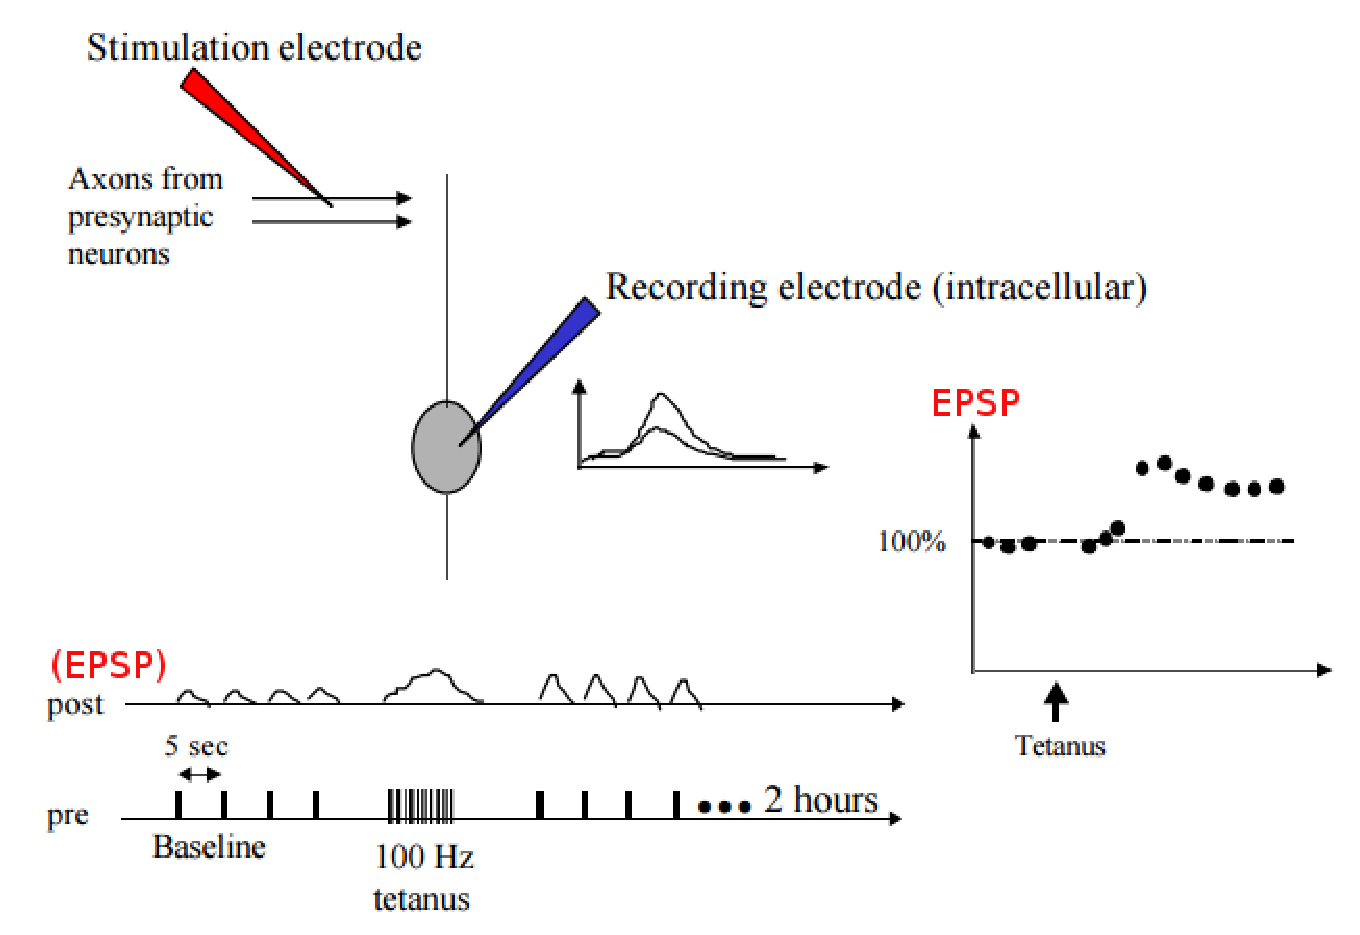
\includegraphics[height=6cm]{./images/frequency-dependent_plasticity.eps}}
  \caption{Frequency dependent synaptic plasticity.
  (Baseline - 0.1Hz stimulus) the recording show the summation of activity of a
  few synapses, (Tetanus stimulus) during tetanus stimulation at one brain
  region projecting onto the neuron in another region, almost all the spines are
  affected by the stimulation which somehow cause a change in synaptic
  plasticity at all synapses for that region-to-region pathway, (0.1Hz stimulus)
  after that summation of activity of a few synapses (about the same number as
  before recorded in (A)) increase (i.e.
  LTP).
  \textcolor{red}{The tetanus phase is often not shown (right plot)}}
  \label{fig:frequency-dependent_plasticity}
% http://www.nbb.cornell.edu/neurobio/linster/BioNB420/hebb.pdf
\end{figure}

 
%\subsubsection{LTP}


\textcolor{red}{A
synapse whose plasticity exposes the following properties is called Hebbian synapse}.
The correlation between the pre- and postsynaptic activity is a function of
\begin{enumerate}
  \item time-dependent: 
  
  The modification of a Hebbian synapse depends on the exact time of occurrence
  of pre- and postsynaptic activity. However, the order of the events between
  pre- and postsynaptic is not important.
  
  \item highly local:
  
  A Hebbian synapse uses this locally available information to cause a local,
  input-specific synaptic modification. This is considered an {\it unsupervised
  form of learning}, as there is no external teacher signal is required.
  
  However, the idea of a local mechanism does not exclude some form of
  neuromodulatory control over the modification process. A "reinforcement
  signal" is not excluded.

  \item strongly {\it interactive mechanism} to increase synaptic efficacy
  
  Palm (1982) pointed out that a Hebbian synapse depends on activity levels on
  both sides of the synaptic cleft. Palm made a distiction between the
  \textcolor{red}{interactive vs. noninteractive mechanism}.
  
  In {\it noninteractive mechanism}, or rules, the presynaptic and postsynaptic
  modification can occur independently, i.e. can be purely presynaptic, purely
  postsynaptic, or a superposition of these, but there is no true interaction.
\end{enumerate}

Hebb (1949) however did not pointed out whether (1) coincidence of pre- and
postsynaptic activity is sufficient to cause modification of synaptic strength,
or it also implies (2) the requirement for a positive (temporal) correlation
between pre- and postsynaptic activity. 

In a later publication, Sejnowski's (1977) formalized Hebb's postulate in
that correlation over time between pre- and postsynaptic activity is responsible
for changes in synaptic efficacy, expressed mathematically as covariance between
pre- and postsynaptic activity. Thus, Hebbian synapse is also called {\bf
correlational synapse} (Anderson 1985).

\subsection{ -- Stent's extension for Hebbian synapse: Stent's mechanism for
synaptic depression}

\textcolor{red}{How about the consequence of uncorrelated or negatively
correlated pre- and postsynaptic activity} (review: \citep{brown1990}).

The idea that positively correlated activity causes synaptic strengthening and
that either uncorrelated or negatively correlated activity causes synaptic
wcakening was in fact an essential part of Stent's (1973) extension of the
Hebbian idea.

Functional coupling can be increase by reducing the strength of inhibitory
synapses activated at the same time  that APs are fired in the postsynaptic
cell. 



\subsection{+ anti-Hebbian learning: long-term depression (LTD)}
%\subsection{Anti-Hebian learning}
\label{sec:anti-Hebbian-learning}

Assuming the original definition of Hebbian learning
(Sect.\ref{sec:Hebbian-learning}), we can define anti-Hebbian learning as a form
of synaptic plasticity where correlated activation in the pre- and postsynaptic
neurons leads to the reduction in the efficiency of the presynaptic neuron's
ability to elicit activation of the postsynaptic neuron \citep{choe2014}.

In anti-Hebbian learning, LTD occurs, where low-frequency stimulation
causes a prolonged decrease in synaptic efficacy -
Sect.\ref{sec:long-term_depression}.

\begin{verbatim}
pre-stimulus phase:
     (stimulate a few synapses) - measure EPSP (baseline)
	 (not enough to trigger spike in postsynaptic neuron)

firing phase: low frequency presynaptic stimulation or weak stimulation
 (that lead to spike in the postsynaptic neuron)
   0.5Hz - 3Hz for 15 seconds or
   weak stimulation

measuring phase:   
 (stimulate a few synapse at 0.1 Hz) - measure EPSP each time
  EPSP is maintained at a lower level --> LTD
\end{verbatim}

It has been shown that LTD can be induced by prolonged {\bf low frequency} (0.5
to 3 Hz), {\bf weak stimulation} of excitatory synapses \citep{dudek1992}.

Palm (1982a,b) has suggested a formalism for classifying what he calls
\begin{enumerate}
  \item {\bf Hebbian synaptic modification}
  
  A Hebbian synapse increases its strength with correlated pre- and postsynaptic
  activity and decreases its strength with negatively correlated activity.

  \item {\bf anti-Hebbian synaptic modification}
  
  An anti-Hebbian synapse rewards negatively correlated activity and punishes
  (positively) correlated activity.
  
  The term "anti-Hebbian", however, is not being used consistently in the
  literature.
  \begin{itemize}
    \item Callaway et al (1987) uses this term to describe changes at neuromuscular
     junction during development
     
     \item Levy \& Desmond (1985) uses this term to refer to a rule
     that decreases synaptic efficacy if postsynaptic activity is unaccompanied
     by presynaptic activity 
  \end{itemize}

\begin{mdframed}

In both Hebbian and anti-Hebbian synaptic modifiaction, modification of synaptic
efficacy involves a real-time, local, and interactive mechanism.
\end{mdframed}  

  \item {\bf non-Hebbian synaptic modification}:
  Sect.\ref{sec:non-Hebbian-learning}
  
\end{enumerate}

\subsection{ -- anti-Hebbian synapses: LTD}
\label{sec:anti-Hebbian-synapse}

Synapses operating under the control of an LTD anti-Hebbian learning
rule (Sect.\ref{sec:anti-Hebbian-learning}) is thought to occur in the
\textcolor{red}{cerebellum} and also in the electrosensory lobe (ELL) in the teleost electric
fishes.
\url{http://icwww.epfl.ch/~gerstner/SPNM/node71.html}

%\subsection{Anti-Hebbian plasticity: LTD}
%\subsubsection{LTD}

\subsection{HFS-LTP}
\label{sec:HFS-LTP}

This is observed in striatum (corticalstriatal SPN, MSN) \citep{fino2005}.

\begin{enumerate} 
  \item Baseline measurement: (Cortical) Currents were adjusted to
evoke striatal EPSCs ranging from 50 to 200 pA amplitudes. Repetitive
control stimuli were applied at a frequency of 0.1 Hz, a frequency for
which no short- and long-term changes in EPSCs amplitudes were induced.
  
  \item Induction phase: highfrequency stimulation (HFS) (train of 1 s duration at 100
Hz repeated four times, separated by 10 s)

Hebbian mode: the depolarization of the postsynaptic element from its resting
membrane potential (RMP) to some value (e.g. -50mV, -20mV, 0mV) was coincident
with the presynaptic stimulation.

non-Hebbian mode: the postsynaptic element being maintained at its RMP during
the presynaptic stimulation.

  \item Measurement: same protocol at firt phase, and compare the change
\end{enumerate}

Early data showed that clamped postsynaptic membrane potential at -20 mV for
LTD, and accounted this for full activation of NMDAR.

\citep{fino2005} applied the induction phase in 2 different scenarios:
Hebbian mode (at 0mV) and non-Hebbian mode (Sect.\ref{sec:Hebbian-mode}). The
result show EPSC is the result of monosynaptic transmission
\begin{enumerate}
  \item non-Hebbian mode (success rate 80\%): LTP $\Delta$ EPSC about 120\%
  increase
  
  The analysis of EPSC (Sect.\ref{sec:EPSC}) shows 
  \textcolor{red}{non-Hebbian HFS-LTP appeared
  to display mainly a presynaptic origin.}
  
  \item Hebiian mode (success rate 79\%): LTP with $\Delta $ EPSC about 150\%
  increase
  
  The analysis of EPSC (Sect.\ref{sec:EPSC}) shows 
  \textcolor{red}{Hebbian HFS-LTP appeared
  to display mainly a presynaptic origin.}
  
\end{enumerate}
In two modes, the slope of changes after induction phase are about the same.
\subsection{B-HFS-LTP}
\label{sec:bHFS-LTP}

Brief high-frequency stimulation (B-HFS) can induces LTP postsynaptically in

A weak burst of synaptic stimulation with a brief dendritic exogenous
  BDNF application: Brain-derived neurotrophic factor (BDNF)-mediated LTP in
  hippocampal neurons requires activation of postsynaptic voltage-activated
  $\Ca$ channels. QUESTION: \textcolor{red}{Can we get the same LTP phenomenon
  induced by endogenous BDNF? the site of endogenous BDNF release? does
  presynaptic TrkB receptors involve in synaptic transmission and plasticity?}
  
  The experiment on presynaptic perforant path fiber originating from cortical
  neurons which form synapse with dentate granulle cells.
  BDNF application alone has no effect on synaptic transmission. However, when
  it is combined with a weak burst of presynaptic activity that itself has
  little effect on synaptic transmission, persistent enhancement of synaptic
  transmission is induced, similar to that seen with tetanic stimulation.
  


MECHANISM: It was suggested that  endogenous BDNF binds to TrkB receptors; but
it was unsure it affects presynaptically or postsynaptically. The study by
Kovalchuk et al. (2002) showed that postsynaptic BDNF-TrkB pathway is crucial
for regulation of excitatory synaptic transmission and LTP.
In mouse hippocampal slices, they found BDNF-evoked $\Ca$ transients in
dendrites and spines, but not at presynaptic sites \citep{kovalchuk2002}.
By voltage clamp to block depolarization on postsynaptic membrane can prevent
this LTP.
So, it was suggested that activated TrkB depolarize the membrane which trigger
the opening of $\Na$ channel and concomitant activation of Ca2+ channels,
resulting in an increase in the Ca2+ concentration.
Also, postsynaptic cell depolarization caused by the activation of TrkB
receptors enhances NMDA receptor opening by removing a Mg2+ block from the
receptor channel

\subsection{LFS-LTD}
\label{sec:LFS-LTD}

This is observed in striatum (corticalstriatal SPN, MSN) \citep{fino2005},
Schaffer collateral-CA1 synapse in the hippocampus \citep{dudek1992, dudek1993}.

% Dudek, S. M. & Bear, M. F. (1992) Proc. Natl. Acad. Sci. USA 89, 4363-4367.
% 2. Dudek, S. M. & Bear, M. F. (1993) J. Neurosci. 13, 2910-2918

\begin{enumerate} 
  \item Baseline measurement: (Cortical) Currents were adjusted to
evoke striatal EPSCs ranging from 50 to 200 pA amplitudes. Repetitive
control stimuli were applied at a frequency of 0.1 Hz, a frequency for
which no short- and long-term changes in EPSCs amplitudes were induced.
  
  \item Induction phase: low stimulation (LFS) (train of 600 s duration at 1
Hz)

Hebbian mode: the depolarization of the postsynaptic element from its resting
membrane potential (RMP) to some value (e.g. -50mV, -20mV, 0mV) was coincident with the presynaptic
stimulation.

non-Hebbian mode: the postsynaptic element being maintained at its RMP during
the presynaptic stimulation.

  \item Measurement: same protocol at firt phase, and compare the change
\end{enumerate}

Early data showed that clamped postsynaptic membrane potential at -50 mV for
LTD, and accounted this for partial activation of NMDAR.

\citep{fino2005} applied the induction phase in 2 different scenarios:
Hebbian mode  (at 0mV) and non-Hebbian mode (Sect.\ref{sec:Hebbian-mode}). The
result show EPSC is the result of monosynaptic transmission
\begin{enumerate}
  \item non-Hebbian mode (success rate 80\%): LTD $\Delta$ EPSC about -40\%
  decrease
  
  The analysis of EPSC (Sect.\ref{sec:EPSC}) shows 
  \textcolor{red}{non-Hebbian LFS-LTD appeared
  to display mainly a postsynaptic origin.}
  
  \item Hebiian mode (success rate 79\%): LTD with $\Delta $ EPSC about -47\%
  decrease
  
  The analysis of EPSC (Sect.\ref{sec:EPSC}) shows 
  \textcolor{red}{Hebbian LFS-LTD appeared
  to display mainly a postsynaptic origin.}
  
\end{enumerate}

\subsection{HFS-LTD}
\label{sec:HFS-LTD}

The conventional HFS-LTD: high frequency stimulating leads to LTD.
For years, LTD was considered as the unique physiological
form of activity-dependent plasticity at corticostriatal synapses.
Fino et al. (2005) demonstrate that this is incorrect, i.e. in the same
conditions the occurrence of both LTP and LTD at these synapses. 


HFS-LTD  requires dopamine D2 receptor (mGluR) activation, high levels of
intracellular calcium, and retrograde release of endocannabinoids that activate
presynaptic CB1 receptors.
\begin{itemize}
  \item mGluR1 activation trigger PLC (Sect.\ref{sec:PLC})
  \item PLC$\beta$ increase Ca2+ sensitivity of IP3R
  \item opening of IP3R increaess $[\Ca]_i$ 
  \item increase $[\Ca]_i$ trigger the release of endocannabinoids (eCB) from
  postsynaptic side
  \item eCB diffuses and activate pre-synaptic side CB1 receptor (CB1R)
  \item activation of CB1R reduces pre-synaptic neurotransmitter release
  (glutamate or GABA depending on the synapse type)
\end{itemize}

Blockade or genetic deletion of dopamine D2 receptors causes loss of HFS-LTD
(Reynolds and Wickens, 2002). Dopamine-dependent changes in synaptic efficacy of
corticostriatal terminals has been shown by many groups.

A D1-type receptor-mediated pathway also has been implicated in HFS-LTD
(Centonze et al., 2003)

\subsection{ * anti-Hebbian LTP}

In some cases, LTP can also be associated with a form of anti-Hebbian learning,
when LTP is induced not by correlated activation but by {\it presynaptic firing
not being met by or negated by the postsynaptic activity}.
Such a phenomenon has been observed in the hippocampus and has been
dubbed {\bf anti-Hebbian LTP}. \citep{choe2014}.

Example: STDP LTP.


\subsection{Spike timing-dependent synaptic plasticity: t-LTP, t-LTD}
\label{sec:spike-timing-dependent-plasticity}
\label{sec:STDP}
\label{sec:t-LTP}
\label{sec:t-LTD}

There are three types:
\begin{enumerate}
  \item  classical STDP (Hebbian STDP) - Sect.\ref{sec:STDP-classic}
  
  \item anti-Hebbian STDP - Sect.\ref{sec:STDP-reverse}
  
  \item bidirectional STDP - Sect.\ref{sec:STDP-bidirectional}
\end{enumerate}

The change in synaptic plasticity as a result of the timing difference between
presynaptic stimulation and postsynaptic backpropagating AP (bAP -
Sect.\ref{sec:back-propagating_AP}) is aka spike timing-dependent synaptic
plasticity.
bAPs decrementally back-propagate into dendrites, providing sufficient
depolarization to open voltage-dependent Ca2+ channels at synapses in the
proximal portion of the SPN dendritic tree (Carter and Sabatini 2004; Day et al.
2008).
% STDP-LTD is the result of the temporal convergence of synaptic input and
% back-propagating action potentials (bAPs) -
% Sect.\ref{sec:back-propagating_AP}.

STDP experiments consisted in time shifting the presynaptic stimulation
($t_{\pre}$) with the time for a postsynaptic action potential (AP) evoked by
application of suprathreshold depolarizing current pulse
($t_{\post}$) (Sect.\ref{sec:STDP-protocol}).

This temporal window $\Delta t = t_{\pre} - t_{\post}$ is narrow and cell
type-specific for such synaptic modification and that the generally accepted
input- (or synapse-) specific rule for  modification appears  not to be 
strictly adhered  to.

\begin{mdframed}

+
Hebbian plasticity requires high frequency of stimulation
(Sect.\ref{sec:Hebbian-plasticity}). 
However, AP firing is sparse in both cortical and striatal spiny projection
neurons {\it in vivo}, with single spikes occurring often; the high-frequency
stimulation-based protocols may not translate well to {\it in vivo}-like
activity. Thus, a novel mechanism - {\bf spike timing-depdendent plasticity}
(STDP) is now accepted as a likely candidate for eliciting changes in synaptic
efficacy between neurons {\it in vivo}.


For STDP, the order and the precise timing of presynaptic $(t_{\pre})$ and
postsynaptic $(t_{\post})$ activation determines LTP and LTD.

\end{mdframed}

In MSN, early data suggested D1 DA receptor signaling promotes long-term
potentiation (LTP) whereas D2 DA receptor signaling promotes long-term
depression (LTD). However, this was proved wrong, as STDP is bidirectional
\citep{shen2008}, i.e. we can reset a synapse in LTD (or LTP) to naive state
from that it can switch to either LTP or LTD in future synaptic modification.
\citep{fino2005} first found {\bf bidirectional STDP} in MSN
(Sect.\ref{sec:homeostatic-plasticity}).

The net change in synaptic strength is hypothesized to reflect the interaction
between cellular processes sensitive to the timing of pre- and postsynaptic
activity (e.g., NMDA receptors, Ltype Ca2+ channels) and G-protein coupled
receptor (GPCR) regulated intracellular signaling cascades.



\citep{bi2001} studies two aspects: (1) temporal specificity (the importance
of temporal order in pre-synaptic and postsynaptic spiking?) and (2) spatial
specificity (do only activated synapse got modified?).
\begin{itemize}
  \item In Hebb's learning: cell A has to fire before cell B to modify the
  synapse of cell B, which is explained by LTP.

New evidences suggest a 'critical window' of spike timing, with precision in the
order of milliseconds. This precise profile of critical window depends on the
synapse type. The window for modification is about 40 ms in width and is
temporally asymmetric. Postsynaptic spiking within about 20 ms after presynaptic
activation (positive intervals) results in LTP, whereas that within about 20 ms
before presynaptic activation (negative intervals) results in LTD.

In hippocampal cultures, GABAergic transmission can also be modified by
correlated pre- and postsynaptic spiking. Such modification exhibits a symmetric
spiking-timing window that lasts about 50 ms and is independent of
N-methyl-Daspartate receptors (NMDARs).

  \item the spatial specificity: 

  LTP of the weak input could be induced when the strong input from another
synapse was activated concurrently with, or following the activation of, the
weak input by as much as 20 ms. When the temporal order was reversed (i.e. postsynaptic occur 20ms
before presynaptic firing), long-term depression (LTD) was induced.

\end{itemize}

A critical factor in classical Hebbian plasticity is the frequency at which the
inputs are recruited. High-frequency stimulation (``tetanization'') leads to
LTP, whereas low frequencies yield LTD. Brief high-frequency stimulation results
in strong postsynaptic depolarization and NMDA receptor activation, whereas
sustained low-frequency stimulation evokes less NMDA receptor-dependent Ca2+
influx.

Indeed, thalamic relay neurons are known to convey information to the neocortex
using both bursts and individual spikes. Very low firing rates are also often observed
during natural in vivo conditions.

In agreement with the view that single spikes convey important information in
neocortical circuits, repeated single spike pairings delivered at very low
frequencies are also quite efficient at eliciting LTP and LTD under many
circumstances. This is called {\bf spike timing-dependent plasticity} with
modeling is discussed in Sect.\ref{sec:spike-timing-dependent-plasticity_model}.

backpropagating postsynaptic spikes indeed can function as an associative signal
for synaptic modification, and relative timing of pre- and postsynaptic activity
is critical.

\subsection{-- STDP experimental protocol}
\label{sec:STDP-protocol}


\citep{fino2010} extracted somatosensory cortex (layer V) and striatum, and
recorded data at 34$^\circ$C.
\begin{enumerate}
  \item LTP and LTD is not a function of stimulation intensity (tested from 50
  pA to 200 pA current injection)
  
  \item experiments:
  \begin{enumerate}
    \item baseline measurement (control stimuli - no LTP or LTD occur): stimuli
    is applied to the cerebral cortex at 0.1 Hz, then measured EPSC for 10min
    
    Electrical stimulations of the cerebral cortex were performed with a bipolar
    electrode placed in layer 5 of the somatosensory cortex. Currents injected
    to cortical neurons were adjusted in order to evoke striatal excitatory
    postsynaptic currents (EPSCs) ranging from 50 to 200 pA amplitudes (Fig.1B).
    
    To make sure the baseline experiment is correct, EPSC is recorded and
    average every 2 min, and if the variation of EPSC amplitude (comparison of 5
    values) greater than 30\%, then the experiment is rejected.
    
    \item induction phase: 100 times of pairing (pre-post) at 1Hz with a time shift
      $\Delta t = t_{\pre} - t_{\post}$ of several miliseconds
      
      NOTE: Pre-synaptic stimulation = cortical stimulation (same amplitude as
      base line phase, just with different frequency), Post-synaptic stimulation
      = direct current injection to MSN for 30 ms (enough to trigger MSN's spike
      and the bAP can remove $\Mg$ block of NMDAR - Sect.\ref{sec:NMDAR-Mg-block}).
      $t_{\pre}$ = time of stimulation artifact in presynaptic neuron, $t_{\post}$ =
      time of peak at postsynaptic AP (soma).
      
            
%     \begin{itemize}
%       \item 
%       \item LTD: 100 times of pairing (post-pre) at 1Hz with a time shift
%       $\Delta t = t_{\pre} - t_{\post}$ of several miliseconds
%       
%     \end{itemize}
    
    \item measuring phase: apply the same control stimuli (0.1Hz)
    and recording for 60 min.
  \end{enumerate}
  
  
\end{enumerate}
% See the case for corticostriatal synapse (Fino et al., 2010) -
% Sect.\ref{sec:corticostriatal-synaptic-plasticity}

{\bf STDP Protocol}:
\begin{itemize}
  \item a synapse is activated by stimulating the presynaptic neuron (or
  presynaptic pathway) shortly before or shortly after making the postsynaptic
  neuron fire (by injection of a short current pulse).
  
  \item this pairing protocol is repeated for 50-100 times at a fixed frequency.
  
  \item the weight of the synapse is then measured as the amplitude (or initial
  slope) of the postsynaptic potential (Sect.\ref{sec:postsynaptic_potential})
  
  \item STDP function: the change in synaptic weight $\Delta w_{ij}$ is plotted
  vs relative timing $\Delta t$ between presynaptic spike arrival and postsynaptic firing,
  Fig.\ref{fig:STDP_plot}. \textcolor{red}{different synapse types can have
  quite different forms of STDP function}.

\textcolor{red}{A sharp discontinuity is observed at 0 ms where differences of a
few milliseconds can determine whether maximal LTP or LTD is induced.}
\end{itemize}

\begin{figure}[htbp]
\centerline{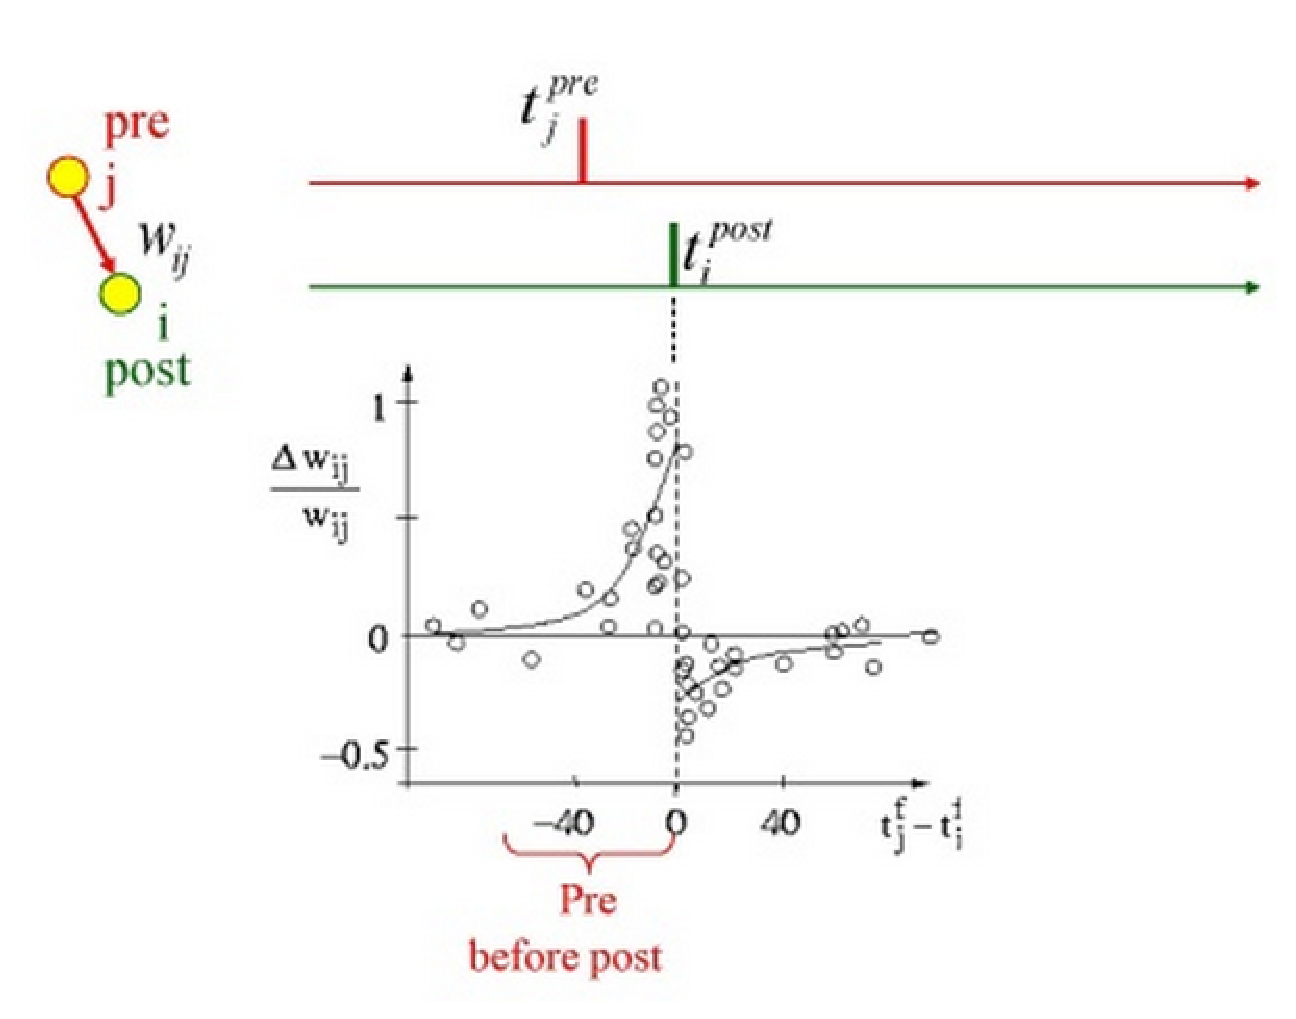
\includegraphics[height=6cm]{./images/STDP_plot.eps}}
\caption{STDP function shows the change of synaptic connections as a function of
the relative timing of pre- and postsynaptic spikes after 60 spike pairings}\label{fig:STDP_plot}
%http://www.scholarpedia.org/article/Spike-timing_dependent_plasticity#fig:STDP-Fig1.JPEG
\end{figure} 


\subsection{-- temporal symmetrical STDP}

Temporal symmetrical STDP
\begin{itemize}
  \item  $|t_{\pre}-t_{\post}| \le \Delta t_1$ then LTP
  \item $\Delta t_1 \le |t_{\pre}-t_{\post}| \le \Delta t_2$ then LTD
\end{itemize}

The spike from postsynaptic side caused by the back-propagation AP can adjust
the synaptic plasticity if it coincide with the presynaptic firing (EPSP) within
a short-enough time interval.

The voltage dependence and ion selectivity of NMDARs provide them with
regenerative properties that allow the generation of dendritic action potentials
(NMDA spikes) that do not originate from bAPs, but from highly synchronized
excitatory synaptic inputs to a region of the dendrite \citep{schiller2000,
schiller2001, enoki2004, gordon2006}.
  
  
\subsection{-- temporal asymmetrical STDP}

\subsection{++++ classic STDP (Hebbian): LTP (pre-post), LTD (post-pre)}
\label{sec:STDP-classic}


Classical STDP has been described in different mammalian brain structures
(Markram et al. 1997;Magee \& Johnston, 1997; Bi \& Poo, 1998; Debanne et al.
1998; but see Bell et al. (1997) in the cerebellum-like structure of the
mormyrid electric fish.
Other types - Sect.\ref{sec:STDP}.

Classical models for STDP propose NMDAR (Sect.\ref{sec:NMDAR}) as the unique
coincidence detector (Nishiyama et al. 2000, Shouval et al., 2002).
Yet, the involvement of multiple coincidence detectors to induce STDP has been
reported (Sjostrom et al. 2003; Bender et al. 2006; Nevian \& Sakmann, 2006).

The review \citep{bi2001}
\begin{itemize}
  \item Bi-Poo (1998) in dissociated culture
  \item Debanne et al. (1998) organotypic slice cultures 
  
  \item  Nishiyama et al. (200) pairing Schaffer collateral stimulation with
  single post synaptic spikes in CA1 region of hippocampal slices from young
  adult rats
  
  They observed two windows for LTD in homosynaptic input: from -28ms to -16ms
  (LTD), and from +15ms to +20ms (LTD)
  
  At Schaffer collateral synapses in the CA1 region of rat hippocampal
slices, LTP/LTD can also be induced with induction protocol of low frequency 5Hz

\item (Markram et al. 1997;Magee \& Johnston, 1997; Bi \& Poo, 1998; Debanne et
al.1998)

\end{itemize}

The induction protocol is given in Sect.\ref{sec:STDP-protocol}

Classic STDP
\begin{itemize}
  \item  LTP: Postsynaptic spiking within about 20 ms after presynaptic
  activation (positive intervals) results in LTP,
  \item LTD: 
Postsynaptic spiking within about 20 ms before presynaptic activation (negative
intervals) results in LTD
\end{itemize}
Classical models for STDP propose NMDA receptors (NMDARs) as the unique
coincidence detector (Nishiyama et al. 2000; Shouval et al. 2002)

% \subsection{ * STDP : LTP (pre-post pairing)}
% \label{sec:STDP_LTP-protocol}

% 
% \subsection{ * STDP : LTD (post-pre pairing)}
% \label{sec:STDP_LTD-protocol}


\subsection{++++ reverse STDP (anti-Hebbian): LTP (post-pre), LTD (pre-post)}
\label{sec:STDP-reverse}

Other types - Sect.\ref{sec:STDP}. Reversed STDP has been reported in 
\begin{itemize}
  \item cerebellum-like structure for mormyrid electric fish: Bell et al. (1997)
  
  \item dorsal cochlear nucleus in rodents: Tzounopoulos et al. (2004, 2007)
  
  \item corticostriatal MSN: \citep{fino2005}
\end{itemize}
% See the case for corticostriatal synapse (Fino et al., 2010) -
% Sect.\ref{sec:corticostriatal-synaptic-plasticity}.

Reversed STDP refers to STDP of anti-Hebbian learning learning rule, i.e.
post-pre leads to LTP and pre-post lead to LTD. This is different from classical
STDP (Sect.\ref{sec:STDP-classic}).




Based on the protocol in Sect.\ref{sec:STDP-protocol}, reversed STDP in
corticostriatal synapse 
\begin{enumerate}
  \item post-pre pairing: LTP with success rate 53\%, for
  time interval $\Delta t = t_{\pre} - t_{\post}$ in -7 ms to -40 ms
  
  average 141\% increase in EPSC. 
  \textcolor{red}{reversed STDP-LTP has presynaptic change origin }
  
  \item pre-post pairing: LTD with  success rate 67\%, for time interval
  $\Delta t	$ in 5 ms to 37 ms
  
  average -25\% decrease in EPSC.
  \textcolor{red}{reversed STDP-LTD has postsynaptic change origin }

\end{enumerate}

In STDP protocols, being less drastic than HFS and LFS protocols, long-term
synaptic efficacy changes might be induced by more subtle intracellular
mechanisms, which need {\bf longer delays to be fully established}.


% \subsection{ * STDP : LTP (post-pre pairing)}
% \label{sec:STDP_LTP-protocol}

% \subsection{ * STDP : LTD (pre-post pairing)}
% \label{sec:STDP_LTD-protocol}

\subsection{++++ Bidirectional STDP}
\label{sec:STDP-bidirectional}

It has been widely believed that synaptic plasiticity is unidirectional, i.e.
a synapse (other than baseline) can be either in LTP or LTD; but cannot
both. Recent evidences showed that a synapse can be in either
baseline, LTP, and LTD, depending on the stimulus input and the form of
activation
\begin{itemize}
  \item STDP: pre-post or post-pre
  \item Hebbian stimulus:
  \item GABA input
  \item DA input
  \item GPCR activation (Gq, Gi/o, Gs) 
\end{itemize}
This is called bidirectional plasticity.

This has been observed using STDP protocol in different brain areas.

This bidirectional STDP found in MSNs on rat brain corticostriatal slices whose
spike-timing dependence displayed an anti-Hebbian learning rule (Fino et al.
2005) - sect.\ref{sec:anti-Hebbian-learning}. Other types - Sect.\ref{sec:STDP}.
The spike-timing dependence of induced synaptic plasticities (LTP versus LTD)
was not related to the stimulation intensity.

\begin{enumerate}
  \item when a MSN action potential (AP) was evoked slightly
before cortical activation (post-pre pairing), a robust
LTP was observed

  \item when cortical activity preceded a MSN back-propagating AP (bAP), a LTD
  was induced.
\end{enumerate}

\textcolor{red}{Protocols}:
\begin{itemize}
  \item  Current stimulus to cerebral cortex was adjusted in order to evoke
  striatal excitatory postsynaptic currents (EPSCs) ranging from 50 to 200 pA
  amplitudes.


   \item  {\bf CONTROL} (Baseline): This control stimulus was applied at 0.1 Hz
   so that neither short- nor long-term synaptic efficacy changes in EPSC amplitudes were induced. 

 
   
  \item  {\bf STDP protocols}: consisted in pairings of pre- and postsynaptic
  stimulations (100 times at 1 Hz) with a time shifting ($\Delta $t) of several
  milliseconds.

Presynaptic stimulations: correspond to cortical stimulations 

Postsynaptic stimulation to an AP evoked by a direct application of a
depolarizing current step (30ms duration) in the MSN.

   \item  $\Delta t$:

$\Delta $t was measured as the time interval between the peak of the
postsynaptic AP and the stimulation artifact (due to presynaptic electrical
stimulation) recorded in the MSN. \textcolor{red}{So, both time-points are
recorded in MSN}.

   
   \item Neuronswere recorded for 10 min during baseline (i.e. CONTROL) and for
   at least 60min after the cellular conditioning protocol; 
   
 \begin{verbatim}
 <---CONTROL---><---STDP-induction-protocol--><----CONTROL---->
    |         |                                              /|\
    |         |                                              |
    record baseline                                 record long-term
                                                   synaptic efficacy changes
 \end{verbatim}
 
   \item Drugs can be applied extracellularly or intracellularly
   
   \item Extracellular: Drugs were applied in the bath, after recording 10 min
   of baseline in control condition and 10min before cellular conditioning
   protocol, and were present continuously until the end of the recording

   \item Intracellular: drugs (applied intracellularly through the patch-clamp
   pipette) were allowed to diffuse into the cell during at least 15min before
   starting the recording of the 10 min baseline before the STDP protocol

\end{itemize}


\textcolor{red}{Studies}
\begin{enumerate}
  \item Blockade of the GABAergic transmission (using Bicuculine) on the
  spike-timing dependence at corticostriatal synapses was studied in Fino et al. (2010)

Role of Dopamine is ignored, i.e. absent. 


  \item 

\end{enumerate}

\subsection{-- burst postsynaptic AP-LTD}

 When paired with trailing synaptic stimulation, repetition of short bAP
bursts at theta frequencies induces LTD in SPNs (Shen et al. 2008).

\begin{mdframed}

In MSN, to generate theta-burst pattern: single bAPs were generated by injecting
current pulses (2 nA, 2 ms) in a theta burst pattern: five bursts, each burst
containing three bAPs with a 20-ms inter-event interval (50 Hz); bursts were
delivered at 5 Hz.

STDP was induced as previously described (Shen et al. 2008): 
\begin{itemize}
  \item Stimulus intensity was adjusted to evoke
baseline single-component EPSPs.
  
  \item Postsynaptic cells were depolarized
to -70 mV, and GABAA receptors were blocked with gabazine
(10 $\muM$).
   
\end{itemize}
Baseline was recorded for 10 min before induction.

INDUCTION PROTOCOL: STDP was induced by pairing a theta burst pattern of
somatically induced APs (as described above) with timed synaptically evoked
EPSPs: $t_1$ (bAP arrive), and $t_1 + \Delta t$ (evoked EPSP arrive)
\begin{itemize}
  \item $\Delta t = 10$ (ms): negative timing protocol
  
  \item $\Delta t = -5$ (ms): positive timing protocol 
\end{itemize}
The induction protocol was repeated 15 times at 0.1 Hz
\end{mdframed}

This spike timing-dependent plasticity (STDP)-LTD has all the pharmacological
properties of conventional HFS-LTD, suggesting that the underlying mechanisms
are the same (Kreitzer and Malenka 2008; Lovinger et al. 2003; Shen et al. 2008;
Surmeier et al. 2009).
\begin{enumerate}
  \item opening of voltage-dependent Ca2+
channels is thought to facilitate STDP-LTD induction by increasing
mGluR-stimulation of phospholipase C (PLC) (Nevian
and Sakmann 2006): pyramidal neurons

  \item or increasing cytosolic inositol trisphosphate (IP3) or activating
src kinase mGluRs promote Ca2+-induced Ca2+ release
(CICR) triggered by opening of voltage-dependent channels
(Berridge 1998; Lerner and Kreitzer 2012; Nakamura et al.
1999, 2000; Nishiyama et al. 2000).
  
  \item MSN: Endocannabinoid (eCB)-mediated corticostriatal LTD
   
  mGluR signaling and activity-dependent Ca2+ entry through L-type
Ca2+ channels would work in concert to elevate postsynaptic Ca2+ concentration
into a range necessary to drive eCB generation

This model suggests that repetition, rather than precise timing of pre- and
postsynaptic activity, is critical to LTD induction. \citep{plotkin2013}


\end{enumerate}

\subsection{-- FPL-LTD (eCB-LTD)}
\label{sec:FPL-LTD}

Here, it shows that there is no need for D2 receptor activation to induce LTD.
The key is in L-type Vm-dependent Ca2+ channel.
To test this, they use
2,5-dimethyl-4-[2-(phenylmethyl)benzoyl]-1H-pyrrole-3-carboxylic acid methyl
ester (FPL 64176, FPL) which is L-type Vm-dependent Ca2+ channel (L-VDD)
activator.
Like HFS-LTD (Sect.\ref{sec:HFS-LTD}), FPL- LTD required postsynaptic
depolarization, increased intracellular calcium, and activated L-type calcium
channels because  hyperpolarization,  intracellular perfusion of BAPTA, and
blockade of L-type calcium channels blocked FLP- LTD.

There is no need for mGluR1 involve, i.e. blockade of mGluR1 receptors failed to
block FPL-LTD, suggesting that strong activation of L-type calcium channels can
override the requirement for PLC-dependent calcium release.
Blocking PLC (Sect.\ref{sec:PLC}) also did not block FPL-LTD.


In corticostriatal MSN, FPL-LTD signaling cascades
\begin{itemize}
  \item FPL activates L-VDCC which then increase $[\Ca]_i$
  
  \item Ca2+ triggers the release of postsynaptic eCB (endocannabinoid) -
  Sect.\ref{sec:endocannabinoid}
  
  \item eCB diffuse and bind to pre-synaptic CB1R (Sect.\ref{sec:CB1R})

  
  \item CB1R inhibit Vm-gated $\Ca$ channels on presynaptic side, reducing
  $[\Ca]_i$ inside the bouton of presynaptic side. 
  
  \item $\Ca$ is important for neurotransmitter release, i.e. reducing
  $\Ca$ also reduce a presynaptic release

blockade of CB1 receptors blocked induction of FLP-LTD.
  
  FPL also produced a gradual increase in the paired-pulse ratio, suggesting
that synaptic depression was attributable to a reduction in presynaptic release
of neuro- transmitter.

\end{itemize}
The basic mechanisms for FPL-mediated eCB signaling are the same at
glutamatergic and GABAergic synapses: both are blocked by CB1R antagonist
(Sect.\ref{sec:CB1R}). This process of course requires presynaptic stimulation
for the release to occur first, before the reduction can occur.

In corticostriatal MSN, FPL-LTD 
\begin{itemize}
  \item depends on temperature at both glutamatergic and GABAergic synapses
  \item is prevented by intracellular loading of the anandamide transporter
  inhibitor VDM11 (10 $\mu$m) at both glutamatergic and GABAergic synapses

  \item blocked by protein translation inhibitors  at both glutamatergic and
  GABAergic synapses
  
 
  \item {\it at glutamatergic synapse}: required paired-pulse afferent
  stimulation, and postsynaptic depolarization to -50mV.
  
  Single presynaptic spikes can modify [Ca2+]i in spiny projection neurons,
  given that  synaptic inputs occurred within 10-20 ms of the onset of
  spontaneous depolarizations, due to back-propagating action potentials (bAPs)
  from the soma (Kerr and Plenz, 2002, 2004).
  
  induced a dose-dependent decrease in EPSC amplitude recorded from striatal
  medium spiny neurons.
  
  \item {\it at GABAergic synapse}: can be induced even in the absence of
  explicit afferent activation
\end{itemize}
Neuronal firing is vital for eCB release and LTD induction at GABAergic
synapses, but not for short-term depression induced by CB1R agonist
\citep{adermark2009}


\subsection{ * Non-Hebbian learning}
\label{sec:non-Hebbian-learning}

In these "non-interactive" synapses, the modifications can be expressed as
simple superpositions of purely presynaptic or purely postsynaptic rules.

\subsection{ -- Non-Hebbian synapses}
\label{sec:non-Hebbian-synapse}

A non-Hebbian synapse is one that does not rely on a real-time, local, and
interactive mechanism

Two categories of learning rules
\begin{itemize}
  \item those that only strengthen the synapse
  
  \item those that can strengthen or weaken the synapse, depending on the
  relationship between pre- and postsynaptic activity levels.
  
\end{itemize}

The depression of synaptic strength can be of the noninteractive type or any of
several different types of interactions between pre- and postsynaptic activity.
\begin{enumerate}
  \item activity occur on one side of the synaptic cleft but not
  the other: non-coincident pre- or postsynaptic activity
  
  \item the occurrence of pre- and postsynaptic activity that is statistically
  uncorrelated or that is negatively correlated in time.
\end{enumerate} 
% However, there is also other form of learning: {\bf anti-Hebbian learning}
% (Sect.\ref{sec:anti-Hebbian-learning}) which links to the depression of synaptic
% strength.

% Different learning rules are proposed to explain the mechanism of how synaptic
% weight (Sect.\ref{sec:synaptic_plasticity}) changes.







\subsection{Homeostasis synaptic plasticity (HmSP)}
\label{sec:HmSP}
\label{sec:homeostatic-synaptic-plasticity}

The neuron  maintains the stability of neuronal functions through a
coordinated plasticity among subcellular compartments, such as the synapses
versus the neurons and the cell bodies versus the axons.

Homeostatic synaptic plasticity (HmSP) refers to self-stabilizing mechanism
occuring at the synapse, unlike homeostatic plasticity which refers to
self-stabilizing mechanism at regions far from synapses
(Sect.\ref{sec:homeostatic-plasticity}.

One key function of such changes would be {\bf homeostatic regulation} of
long-term spiking activity. If too many excitatory synapses become stronger, the
neuron  might spike too often, causing other neurons to spike too often, and
eventually leading to epileptic seizure.

HmSP encompasses a set of 'rheostat' control mechanisms that are thought to
stabilize firing rates in neural circuits. This is relevant to {\it discharge
frequency} of that neuron (Sect.\ref{sec:discharge-frequency}).

%  HmSP is a form of "rheostat" control mechanism that at both the synaptic and
%  circuitry level maintains a normal operating range to enable synaptic
%  plasticity in the face of
% repeated episodes of alterations such as long-term potentiation or depression.



Fino et al. (2005) showed that a LTP-induced protocol can convert an LTD synapse
to control state, i.e. reseting the synapse, and vice versa (Fig.5).
This avoid synaptic saturation, i.e. it reaches a state of plasticity that
unchanged. So, the LTP-LTD and LTD-LTP sequence revealed the existence of an
efficient homeostatic processes. The question is \textcolor{red}{the biological
mechanisms for this reset occurs?}


% \begin{itemize}
%   \item (i) Can firing rates of single cells be modified? 
%   
%   \item (ii) Once modified, what mechanism(s) can maintain the changes?
% \end{itemize}

   
\textcolor{red}{There are multiple forms of HmSP}
\begin{itemize}
  
  \item {\bf synaptic downscaling}: characterized by a multiplicative decrease
  in the strength of excitatory synaptic inputs to a neuron as a compensatory response 
  to 
  \begin{itemize}
    \item chronic increases in firing rate.
    \item increased glutamatergic transmission
  \end{itemize}
  
chronic activation leads to a compensatory decrease in synaptic responsiveness

  \item {\bf synaptic upscaling}: characterized by a multiplicative increase in
  the strength of excitatory synaptic inputs to a neuron as a compensatory response
  to 
  \begin{itemize}
    \item  Hypothesis I:  chronic reductions in firing rate.
    \item  Hypothesis II: an alternative possibility is that reduced
    glutamatergic transmission generates this plasticity directly.
  \end{itemize}
  However, spiking and neurotransmission are tightly coupled, so it has been
  difficult to determine their independent roles in the scaling process.
  \citep{fong2015} showed that upward scaling is dependent upon
  neurotransmission rather than spiking.
  
  
%chronic inhibition leads to a compensatory increase  in postsynaptic
% responsiveness
\end{itemize}

Presynaptic forms of HmSP are mediated by compensatory increase or decrease of
transmitter release in response to chronic inhibition or activation in
postsynaptic activity, respectively, and involve retrograde signaling from the
postsynaptic side, which ultimately lead to transcriptional alterations in the
presynaptic neuron.

HmSP entails uniform adjustments in the strength of all synapses on a cell
in response to prolonged changes in the cell's electrical activity.
Without homeostatic synaptic scaling, neural networks can become unstable and
perform suboptimally.




\subsection{Non-local Hebbian synaptic modification}
\label{sec:non-local-synaptic-modification}
%\subsection{Hebbian mechanism subjected to global control}

Although a Hebbian mechanism uses only local information, the modification
process may be subject to global control signals.
A global "reinforcement signal" can thus control Hebbian plasticity in a large
population of activated synapses.

There are evidences of activity-induced synaptic modification  that may  be 
accompanied  by  changes  in  some  other  synapses  within  a  neural network.
Spread of LTP/LTD observed in different systems \citep{bi2001} (Table .2)
\begin{itemize}
  \item LTP: 
\end{itemize}


Plausible candidates for this role
\begin{itemize}
  \item neuromodulators: catecholamines (Sect.\ref{sec:Catecholamines}),
  acetylcholine (Sect.\ref{sec:Acetylcholine})
\end{itemize}

% Depending on
% the synaptse (i.e. neuron connection at different regions in the brain), there
% are different

\subsection{Activity-independent synaptic plasticity}
\label{sec:activity-independent-synaptic-plasticity}

The plasticity changes as a result of some fluctuations that does not leading to
a spike in both presynaptic neuron and presynaptic neuron.
\begin{enumerate}
  \item serotonin (5-HT)-dependent synaptic plasticity in hypoglossal (XII)
  motoneurons \citep{bocchiaro2004}
  
  Episodic, but not continuous, activation of postsynaptic 5-HT type 2 (5-HT2)
  receptors (Sect.\ref{sec:serotonin-receptors}) on hypoglossal (XII)
  motoneurons leads to long-lasting increases in their AMPA receptor-mediated
  respiratory drive currents and associated XII nerve motor output.
  
  \item 
\end{enumerate}


\section{The role of input}

\subsection{Dopamine input}


D1 DA receptor signaling promotes long-term potentiation (LTP) (3,7) whereas D2
DA receptor signaling promotes long-term depression (LTD) (8,9).
In animal model of Parkinson's Disease (PD), striatal DA levels are very low,
both forms of synaptic plasticity in MSNs appear to be lost, suggesting that DA
receptor signaling is necessary for their induction.




\subsection{GABA input}

\subsection{\ldots}

\section{Noise in }

A growing number of studies indicate that noise generated by random channel
opening limits neuronal response reliability (Schneidman et al., 1998; White et
al., 2000), influences the energy efficiency of channels (Schreiber et al.,
2002), and constrains the physical dimensions of axon diameters (Faisal et al.,
2005).

Conversely, noise can have a beneficial role by enhancing the
detection of weak periodic signals via a stochastic resonance
mechanism (Wiesenfeld and Moss, 1995) or via enhancing subthreshold
oscillations (Dorval and White, 2005).

It seems likely that the magnitude of channel noise is under evolutionary
pressure in biological systems seeking energy-efficient coding systems (Laughlin
and Sejnowski, 2003). For example: Kole et al (2006) showed that Ih current
generates between $\sim$ 40 and 130 $\mu$V of voltage noise (rms) spatially
distributed from the soma to distal dendrites, with most of the power below 10
Hz. First,
channel noise is greater for voltage-dependent channels, like Ih,
that have slow activation kinetics (Diba et al., 2004). Second,
channel noise increases linearly with channel number (Diba et al.,
2004), and, as we show, Ih channel densities can be very high,
particularly at distal dendritic locations. Third, channel
noise would be expected to lead to larger voltage noise in smaller
compartments in which Ih channel densities are maximal. Finally,
the depolarizing gradient generated by Ih will enhance Na+ channel
noise


Most recent studies have focused on the role of stochastic openings of Na+
channels (Schneidman et al., 1998; Diba et al., 2004; Dorval and White, 2005;
Faisal et al., 2005; Jacobson et al., 2005),



\section{Plasticity in corticostriatal synapse: EC to striatal}
\label{sec:corticostriatal-synaptic-plasticity}

Large portions of the cortex project to the striatum through the corticostriatal
pathway but the axons remain segregated along the pathway and innervate specific
input areas within the striatum.

The striatum is further segregated into dorsal and ventral segments, the caudate
nucleus and the putamen respectively (Sect.\ref{sec:striatum}).

The primary cortical connection of the association loop is the dorsal striatal
compartment
\begin{itemize}

  \item association loop

\begin{verbatim}
  Cortex						dorsal striatum
Pyramidal ----[glutamate]---->  MSN
\end{verbatim}

Most of the information in the dorsal compartment flows though central striatal
regions, such as the head of the caudate.
  
  \item limbic loop: primary cortical connection of the limbic loop is the
  ventral striatal compartment

\begin{verbatim}
  Cortex						ventral striatum
Pyramidal ----[glutamate]---->  MSN
\end{verbatim}

Most of the information in the ventral compartment flows through ventromedial
striatal region.

\end{itemize}

% Unlike the situation at other synapses, striatal LTD induction requires
% pairing of postsynaptic depolarization with moderate to high-frequency
% afferent stimulation at physiological temperatures.
corticostriatal STDP reported so far by (Pawlak \& Kerr, 2008; but see Shen et
al. 2008 in which LTD cannot be induced in MSNs expressing the D1 receptor in
mice).

Before Fino et al. (2005), {\it in vitro} corticostriatal transmission has been
studied by stimulating the corpus callosum or the striatum itself, which means
it can trigger other projections (e.g. GABAergic, serotoninergic, dopaminergic,
cholinergic, and noradrenergic projections).

Fino et al. (2005) for the first time, showed an experiment by stimulating the
layer V of cortex, and thus enable only the activation of corticalstriatal
synapse. They also showed the record EPSC is the result of monosynaptic
transmission. 

The synaptic plasticity is bidirectional (Sect.\ref{sec:STDP-bidirectional}),
i.e. it becomes LTP or LTD depends on induction protocol
\begin{itemize}
  \item HFS-LTP
  \item LFS-LTD
  \item reversed STDP:
\end{itemize}




\subsection{* Hebbian mode (Hebbian protocol) vs. non-Hebbian mode
(non-Hebbian protocol)}
\label{sec:Hebbian-mode}

MSN are characterized by a very hyperpolarized resting Vm, and are maintained by
intrinsic membrane conductances that shunt uncorrelated cortical inputs. So, it
only discharge (i.e. generate spike) when they receive strong and correlated
cortical inputs. Also, during the time of suprethreshold Vm, they can also
receive other cortical signals. The question is how the MSN behave under such
situations?

To explore the two difference scenario, two different experimental protocols
were used \citep{fino2005, fino2010}
\begin{enumerate}
  \item  {\bf Hebbian mode} refers to the experiments that the depolarization of the
postsynaptic element from its resting membrane potential (RMP) to 0mV was
coincident with the presynaptic stimulation.

  \item {\bf A non-Hebbian mode} refers to the experiments that the postsynaptic
element being maintained at its RMP during the presynaptic stimulation.

\end{enumerate}


It should be noted that non-Hebbian and Hebbian terms referred strictly to the
stimulation protocols and the corresponding induced-plasticities and did not
designate underlying induction mechanisms \citep{fino2005, fino2010}.

\section{Plasticity in hippocampal neurons}
\label{sec:hippocampus-synaptic-plasticity}

Ca2/calmodulin protein kinase II (CaMKII) activation by HFS is essential for
hippocampal LTP induction.
The proposed CaMKII hyperactivation under basal conditions was further supported
by results on phospho-Ser-831 of glutamate receptor type 1, which is a
postsynaptic CaMKII target.

HFS increased phospho-CaMKII levels in control mice but did not further induce its
autophosphorylation in JP-DKO mice.

Moriguchi - Takeshima (2006) showed the importance of ER-PM junction, maintained
by JP-3/JP-4 (Sect.\ref{sec:JP-3}) in tuning of excitability and plasticity
in hippocampal pyramidal neurons \citep{moriguchi2006}.


\section{Plastciticy thalamocortical synapse}
\label{sec:cortex-synaptic-plasticity}

Parallel model of basal ganglia circuitry enables maintaing the distinct
corticobasal ganglia loop through projection back to the same area on cortex.
\begin{itemize}
  \item relay function: Thalamic relay nuclei form a crucial link between the basal ganglia and cortex
by transmitting basal ganglia output to specific frontal cortical area.

  \item modulation and regulation function of cortical-cortical activity, by
  projecting to different cortical layers
\end{itemize}

In thalamocortical slice preparations, simultaneous presynaptic stimulation and
postsynaptic depolarization can induce L TP in animals prior to the critical
period. However, Akrong (2009) showed that it can fail to produce either L TP or
LTD in the awake freely moving animal \citep{akrong2009}.



\section{Plasticity perforant pathway synapse: EC to dentate gyrus}
\label{sec:dentate-gyrus-synaptic-plasticity}

The synaptic plasticity of dentate gyrus, i.e. the layer II - dentate gyrus
projection in the perforant pathway ({\it perforant path-dentate granule cell
synapses}) is studied (Sect.\ref{sec:perforant-pathway}). Protocol to induce and
monitor LTP in the dentate gyrus, as described previously (Davis et al., 2000).
\begin{enumerate}
  \item baseline measurement: low-frequency test pulse (100$\mus$, 0.033 Hz)
  were delivered by a photically isolated constant current unit
  
  Wait until the responses has stabilized, measure the baseline for 20 min
  
  NOTE: For the second experiment (to test the effect of blocking PI3K), after
  that 20 min, we add LY294002 5mM  - PI3K inhibitor, and wait for 30 min -
  Sect.\ref{sec:PI3K}.
  
  
  \item induction phase: tetanus stimuli to induce LTP (six trains of pulses
  (400 Hz) delivered at 2.5-ms intervals)
  
  NOTE: Second method for induction: six tetanus stimuli (each 400Hz) delivered
  at 20 second interval.
  
  NOTE: The third method for LTP induction: a single tetanus stimulus of 400Hz
  
  \item LTP measurement: record for 1h
\end{enumerate}

RESULT: From the postsynaptic side (dentate gyrus)
\begin{enumerate}
  \item PI3K inhibition does not block LTP
induced with repeated series of tetanic stimulation suggesting that, with
repeated stimulation, additional in vivo signalling pathways may be activated
that compensate for inhibition of PI3K.

  \item PI3K is required for the maintenance but not the induction of LTP in the
dentate gyrus in vivo using a single tetanus.

\textcolor{red}{What downstream targets of PI3K that involve in LTP
maintenance?} - Sect.\ref{sec:PI3K}. In PIK3-blocked rat (vs. control)
\begin{itemize}
  \item Akt : only phosphorylated at Ser site (not Thr site)
  
  \item FKHR (direct downstream of Akt): increase high after LTP in both cases,
  but mTOR cannot be maintained (i.e. return to basal level at 15 and 60 min)
  
  \item mTOR (direct downstream of Akt): no change (compared to
  significant increase in control case)
  
NOTE: The two proteins FKHR and mTOR requires hyperphosphorylation of Akt which
is not the case in PIK3-blocked LTP-induction, so it suggests they can also be
activated by other mechanism, but to maintain, require Akt full activation.
  
  \item MAP/ERK pathway: no involve in PI3-K blockade of LTP maintenance.
\end{itemize}
\end{enumerate}

IMPORTANT: PI3-K blockade induce deficit in learning and memory.
The study show that inhibition of PI3K had no effect on short-term recognition
memory but did disrupt long-term consolidation of both novel object recognition
and objectplace recognition (Horwood et al., 2006)


\section{Plasticity perforant pathway: EC to hippocampal neuron}
\label{sec:spatial-memory}

The synaptic plasticity in hippocampal pyramidal neuron is believed to be
NMDAR-mediated, and is important for spatial memory. The study on CA1  pyramidal
cells of the hippocampus with the deletion NMDAR1 gene making the mouse
exhibiting impaired spatial memory but unimpaired nonspatial learning.

NMDARs act as coincidence detectors because they require both presynaptic
activity (glutamate released by axonal terminals) and postsynaptic activity
(depolarization that releases the Mg2+ block) as a condition for channel
opening.
\begin{verbatim}
presynaptic ---> GluT              --> NMDAR (event-1)
postsynaptic---> remove Mg2+ block --> NMDAR (event-2)

(event-1)+(event-2)--> NMDAR opening --> Ca2+ influx --> trigger a cascade of
      subcellular signaling events 
\end{verbatim}
\textcolor{red}{It is IMPORTANT to characterize these subcellular signaling
events, and understand their role in changing synaptic plasticity.}


Protocols
\begin{enumerate}
  \item control phase (baseline measurement): stimulate 0.1 Hz to collect stable
  EPSC baseline
  
  \item induction phase: 
  \begin{itemize}

    \item LTP: one train of strong tetanus stimuli (25-100Hz for 1 second) or
    theta burst stimulation

     \item (homosynaptic) LTD: 300 stimuli at 1Hz (presynaptic neuron) and
     paired with holding potential of -40mV on hippocampal neuron
     
    NOTE: If block PI3-K using 10$\muM$ LY294002, it produces LTD in also
    non-conditioned pathway (i.e. heterosynaptic LTD or the LTD is induced in
    the non-conditioned synapse)
  \end{itemize}
  
  
  \item control phase: check the change in EPSC 
\end{enumerate}

RESULTS:
\begin{enumerate}
  \item LTP: NMDAR activation is critical for the induction of LTP
  [blocking NMDAR also block the induction of LTP in most hippocampal synapses]

\textcolor{red}{What downstream target of NMDAR activation?} (NOTE: NMDAR
activation increase $[\Ca]$
\begin{itemize}
  
  \item  deletion in the gene encoding the $\alpha$ subunit of
  calcium-calmodulin-dependent protein kinase II ($\alpha$CaMKII -
  Sect.\ref{sec:CaMKII}) display impaired LTP in the CA1 region of the hippocampus
  and a deficit in spatial learning (Silva et al., 1992).
  
\begin{verbatim}
NMDAR --> [Ca] increase --> Ca2+/CaM --> CaMKII --> phosphorylate GluR1-AMPAR
\end{verbatim}
Sect.\ref{sec:calmodulin} explains the mechanism of Ca2+/CaM complex regulating
target proteins, in this case is CaMKII.
  
%   A Silva, C.F Stevens, S Tonegawa, Y Wang Deficient hippocampal long-term
%   potentiation in alpha-calcium calmodulin kinase II mutant mice Science, 257
%   (1992), pp. 201-206
%  
   
   \item The subunit GluR1 of AMPAR is essential for LTP in the CA1 region of
   the adult hippocampus (Sect.\ref{sec:AMPAR-phosphorylation}) 
   
   There is a significant increase in GluR1 phosphorylation at Ser 831 (CaMKII/
PKC site) at 30min and 1h after the induction by CaMKII \citep{lee2000pab}.
Phosphorylation of Ser 845 (PKA site) was not significantly increased 30 or 60
min after LTP induction.

\end{itemize}


  \item 
\end{enumerate}


Hippocampal LTD is a long-lasting decrease in synaptic strength and is most
commonly studied at glutamatergic inputs to CA1 pyramidal cells

Different forms of LTD in 
\begin{enumerate}
  \item transient activation of NMDAR : leads to decrease in synaptic
  transmission.
  
  It is classified as homosynaptic plasticity, i.e. the depression occurs in
  synapses at which NMDAR were activated, but not at neighboring non-conditioned
  synapses.
    
  \item homosynaptic LTD with a similar mechanism in chemLTD: \citep{lee2000pab}
  although the magnitude of the change in GluR1 phosphorylation following
  homosynaptic LTD was smaller than that reported for chemLTD, because only a
  small percentage of synapses in the slice are depressed during LFS-induced
  homosynaptic LTD.
  
  dephosphorylation of Ser 845 of AMPAR by phosphatase 1/2A (PP1), but not
  phosphorylatation at Ser 831 of AMPAR: be detected as early as 30 min after the onset of LFS
  (Sect.\ref{sec:AMPAR-phosphorylation}). There was no dephosphorylation in
  slices that did not exhibit LTD after LFS. SUGGEST: chemLTD and homosynaptic
  LTD share similar downstream expression mechanism. 
  
\begin{mdframed}

Chemically-induced LTD (chemLTD): associated with persistent
dephosphorylation of GluR1 at a PKA phosphorylation site, Ser 845.
\end{mdframed}
  
\end{enumerate}

\section{Plasticity in Schaffer collateral synapse (CA3 $\rightarrow$ CA1)}
\label{sec:synaptic-plasticity-CA3-to-CA1}

Schaffer collateral synapse: EPSP from CA3 pyramidal cell to CA1 pyramidal cell

Brief high-frequency stimulation (B-HFS) can induces LTP postsynaptically in
Hippocampal mossy fiber project to CA3 pyramidal neuron  \citep{kapur1998}: and require elevation of postynaptic $\Ca$ 
NOTE: Long high-frequency stimulation indeed  induces mossy fiber LTP
presynaptically.

NMDA receptor-dependent LTP in the adult hippocampal Schaeffer collateral-CA1
synapses is the most widely studied type of LTP,  and has been considered the
potentiation mechanism involved in circuit development and adult learning. NMDAR
is discussed in Sect.\ref{sec:NMDAR}.


\section{Plasticity in mossy fiber synapse: granule cell $\rightarrow$ CA3}



\section{Mechanism for Long-term plasticity (mechanisms for memory)}

% Sect.\ref{sec:LTplasticity} have introduced briefly the concept of long-term
% plasticity. In this section, we will discover in details the different
% mechanisms leading to LTP and LTD.
% 



% . Mechanisms are known for excitatory
% inotropic glutamate synapses (Sect.\ref{sec:glutamate_receptor}).

%\url{http://en.wikipedia.org/wiki/Long-term_potentiation}



% \subsection{Hebbian plasticity: LTP + spike frequency}


% \subsection{Brief high-frequency stimulation: LTP (VDCA + NMDA)}
% 
% \begin{itemize}
%   \item 
% 
% 
%   \item 
% 
%   \item 
% \end{itemize}
% 

%\subsection{BDNF-mediated LTP}





% \subsection{Hebbian plasticity (Hebbian  rule: spike frequency-dependent
% plasticity)}
\section{LTP vs. STP}


Short-term potentiation (STP - Sect.\ref{sec:short-term_potentiation}) is
induced by high-frequency stimulation (HFS), but HFS can also induce Long-term
Potentiation (LTP) as in the case of Hebbian LTP plasticity
(Sect.\ref{sec:Hebbian-plasticity}).

So the question is what is the relationship between STP and LTP?
\begin{enumerate}
  \item does STP is the reversible form of LTP elicited by subthreshold stimuli?
  
  \item or does STP  is an independently expressed form of synaptic plasticity
  that differs from LTP?
\end{enumerate}
\citep{schulz1997}

\subsection{Presynaptic modification}

The modification of presynaptic neurotransmitter release (Sect.\ref{sec:presynaptic-side-structure})
can be controlled either from activity of presynaptic terminals ({\it
classical form}) or postsynaptic terminal ({\it novel form} of
activity-dependent synaptic modulation).
\begin{enumerate}
  \item first thought to be controlled by neurotransmitters through {\bf
  autocrine mechanism}
  \begin{enumerate}
    \item in inhibitory synapse: GABA released from GABAergic presynaptic
    terminal can activate GABA$_B$ autoreceptors (Sect.\ref{sec:GABA-receptor-presynaptic})
    on the terminal and thus suppress further GABA release
    
    \item in excitatory synapse: Glutamate released from excitatory presynaptic
    terminal can activate mGluR on presynaptic side (Sect.\ref{sec:mGluR-presynaptic})
    and thus suppress further glutamate release
  \end{enumerate}
 
  
  \item recently found that neurotransmitter release can also be controlled from
  the postsynaptic side via {\bf retrograde signalling} of endocannabinoid
  (Sect.\ref{sec:CB1R}).
\end{enumerate}

\section{Does a synapse possess multiple forms of synaptic plasticity?}

Most synapses possess multiple forms of presynaptic plasticity, and net synaptic
strength reflects an interaction between these forms of plasticity (review:
\citep{regehr2012}). 
\begin{itemize}
  
  \item  Indeed, most synapses can show either
facilitation or depression depending on the initial probability of release.
Often, shortterm depression, facilitation, PTP, and longerlasting depression are
all present. Basic models present these effects as additive, with the sum
creating the net plastic change (facilitation - depression = net change)

The relative prominence of each of the mechanisms is controlled by the initial
release probability and the presynaptic activity pattern.
Example: by altering the extracellular calcium ($[\Ca]_e$) to change
the initial probability of release at climbing fiber-to-Purkinje cell synapse in
cerebellum, Fig.\ref{fig:Role_initial-Pr-in-synaptic-plasticity}.


\begin{figure}[htb]
  \centerline{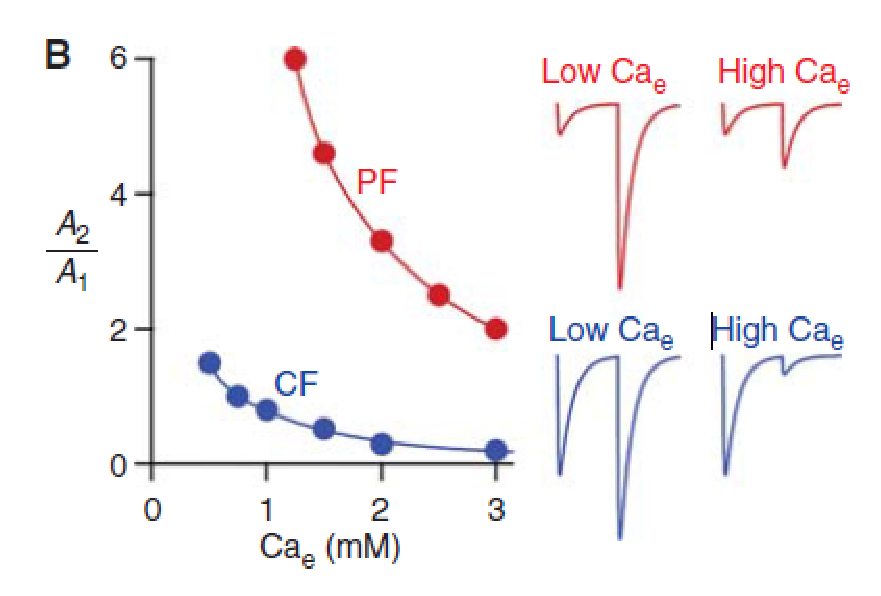
\includegraphics[height=4cm]{./images/Role_initial-Pr-in-synaptic-plasticity.eps}}
  \caption{In PPF, the extent of paired-pulse plasticity depends on the initial
probability of release, and synapses with a high initial probability of release
tend to depress, whereas those with a low initial probability of release usually
facilitate. High $[\Ca]_e$ increase initial probability of release, which
reduces the effect of synaptic plasticity change in (A) facilitation, (B)
depression. Facillitation achieves 6-fold with low $[\Ca]_e$, and much smaller
with high $[\Ca]_e$ }\label{fig:Role_initial-Pr-in-synaptic-plasticity}
\end{figure}
\item 

  \item  
\end{itemize}

\section{Synapse as a filter}

Because the probability of vesicle release is activity-dependent, synapses can
act as dynamic filters for information transmission.
\begin{itemize}
  \item high-pass filter:  Synapses with a low initial probability of vesicle
  release.
  
  a higher-frequency signal is needed to trigger release, and the synapse thus
  selectively responds to high-frequency signals.
  As synapses with low release probabilities are more likely to experience
  facilitation than depression,
  high-pass filters are often converted to band-pass filters.
  Similarly,  it is common for low-pass filters to become band-pass filters, as
  well. 
  
  \item low-pass filter: synapses with high initial release probabilities
  
  \item band-pass filter: Synapses with an intermediate probability of release 
  
  It selectively respond to a specific range of frequencies. 
  
  
\end{itemize}
These filtering characteristics may be affected by a variety of factors.



\section{Experimental techniques}

\subsection{Neurotoxins}

Several neurotoxins have been found great application in the analysis of voltage
and chemically gated channels as well as the process of synaptic transmission.
\url{http://nba.uth.tmc.edu/neuroscience/m/s1/chapter06.html}

\subsection{Single-particle tracking}
\label{sec:SPT}
\label{sec:single-particle-tracking}


Single particle tracking (SPT) is the observation of the motion of individual
particles within a medium \citep{qian1991,saxton1997}. Applications:
\begin{itemize}
  \item used to quantify specific behaviour of a
  protein on the cell surface. 
  
  \item used to understand the cellular kinetics of many proteins 
\end{itemize}

By labeling membrane component of the transmembrane protein with either an
optical label (such as a gold or polystyrene bead) or a fluorescent tag a
trajectory can be observed.
\url{http://en.wikipedia.org/wiki/Single_particle_tracking}





\section{Different training to test memory circuit involved in different task}
\label{sec:test-training-memory}

In animal study, different tests have been proposed to assess animal's behavior
when exposed to a novel vs. a familiar object:
\begin{itemize}
  \item  visual paired comparisons task (VPC) in humans, 
  
  \item the open-field task, 
  
  \item the one-trial novel object recognition (NOR) test,  
  
  \item \textcolor{red}{delayed response (DR) task}: 
  Sect.\ref{sec:delayed-response-task}
  
  \item \textcolor{red}{delayed matching-to-sample (DMTS)} task:
  
  \item  \textcolor{red}{delayed non-matching to sample (DNMTS)}:
  the subject is required to choose the stimulus that does not match the test
  (sample) stimulus that was presented before the recall delay.
  First, given a trial-unique (unfamiliar) sample stimulus for the subject to
  recognize, then with a delay (either 15s, 30s, 60s, 90s) with blank screen
  (remove the sample), and then given both the sample and a novel stimulus item.
  
  
  This task has been used extensively in monkeys to identify the brain regions
  involved in recognizing previously presented stimuli.
  It is thought that monkeys learn to perform DNMTS tasks much more rapidly than
  they learn to perform DMTS tasks because of their natural tendency to
  preferentially attend to novel stimuli, in this case, the non-matching
  stimulus.
  
  If the monkey choose the novel stimulus, a reward is given
  to train the monkey's memory about this task. The study revealed a number of
  interconnected areas involved in the encoding, retention, and retrieval of
  stimulus representations within DNMTS trials.
  (1) ventromedial and ventrolateral prefrontal cortices, (2) rhinal (entorhinal
  and perirhinal) cortex, (3) thalamus, and (4) the inferotemporal cortex.
  The hippocampus, located in the medial temporal cortex, might also be a
  component of this circuit, but its precise role is currently the subject of
  debate.
  
  A growing body of work suggested 2 phases of DNMTS task: (1) dLPFC
  (Sect.\ref{sec:dLPFC}) in DNMTS acquisition, and medial temporal lobe is for
  subsequent DNMTS trials.
   
\end{itemize}
(review: \citep{antunes2012}).

Although recall and recognition are considered separate processes, it should be
noted that they are both most likely constitute components of distributed
networks of brain regions.
PET studies on recall and recognition have showed the increases in
regional cerebral blood flow (RCBF) on these regions:
\begin{enumerate}
  \item prefrontal cortex on right hemisphere
  \item hippocampal and parahippocampal regions of the medial temporal lobe
  \item anterior cingulate cortex
  \item the posterior midline area that includes posterior cingulate,
  retrosplenial (see retrosplenial region), precuneus, and cuneus regions
  \item inferior parietal cortex on right hemisphere
  \item cerebellum on the left side
\end{enumerate}

\subsection{A-not-B task}
\label{sec:A-not-B task}

{\bf A-not-B task} (or A-not-B error or "stage 4 error" or "perseverative
error").

\begin{itemize}
  \item an attractive toy is hidden under box ``A'' within the subject's reach
  (subject = baby < 10 month-old, or monkey)
  
  \item the subject search for the toy, looks under box ``A'' and find the toy
\end{itemize}
This is repeated several times until the region in the brain of the subject is
suppose to hold that information. Then, in a critical trial, the toy is moved to
box ``B'' (with the subject seeing that action), which is also within the reach
of the subject. However, the subject keep searching for toy in box ``A''.
This demonstrates a lack of, or incomplete, schema of object permanence. 
Children from 12months do not make this error.
	
\url{https://en.wikipedia.org/wiki/A-not-B_error}

\subsection{Delayed matching visualspatial task}
\label{sec:delayed-matching-to-visualspatial-task}

The presentation of information contains both image and its location. Example:
during the sample phase of each trial, subjects viewed a novel scene consisting
of four objects (out of a set of nine objects), each in one of nine possible
locations in a 3 x 3 grid.

To test the role of hippocampus in short-term memory, then the test  needs to
make sure hippocampus are used. Thus, to encourage use of a hippocampally
mediated allocentric (or world-centered) strategy, rather than an egocentric (or
viewer-centered) strategy thought to rely on parietal and prefrontal cortices,
subjects were asked to form a mental image of the scene rotated 90$^\circ$ to
the right of the original viewpoint. They were then required to maintain the rotated
representation during the ensuing 11 s delay phase in anticipation of the test
stimulus.

During the test phase, subjects' memory for the positions of the objects was
assessed. This was done by asking them to classify, by button press, the test
stimulus according to whether it constituted (1) a "match" (i.e., the original
scene rotated 90$^\circ$); (2) "mismatch-position" (i.e., one object occupied a new
location); (3) "mismatch-swap" (i.e., two objects had swapped locations").
Performance in all conditions was significantly greater than a chance level of
33\% correct responses: 78, 65, and 60\% on match, mismatch-position and,
mismatch-swap displays, respectively.



\subsection{Delayed matching-to-sample task}
\label{sec:delayed-matching-to-sample-task}



\subsection{Delayed response (DR) task}
\label{sec:delayed-response-task}

{\bf Delayed response (DR) task} is among the most useful tasks in studying
short-term memory in animals (Sect.\ref{sec:short-term_memory}).
It tests {\bf visual-spatial working memory} using 2 phases (baiting and
response) or presentation-delay-response

\begin{itemize}
  \item presentation (baiting phase): one presents a bit of information (a
  sample which can be a sequence of images) to a subject
  
  \item delay: withdraws that information and wait for a certain period of time
  (recall
  delay)
  
  \item response: two ways to test
  (1) presents that same bit of information along with a comparison bit
  and (response phase) asks the subject to identify (choose) which bit of
  information was presented previously
  
  (2) just ask the subject (human) to report the exact information presented
  before the delay. This typically requires 
\end{itemize}
This process is then repeated across a  number of trials.

Nonhuman primates are often used to study the biological underpinning of human
learning and memory processes.

Goldman-Rakic et al. have shown the importance of the {\it prefrontal cortex}
in the performance of DR tasks in nonhuman primates by employing lesions and
electrophysiological and neuroimaging techniques.
Brain lesion experiments in monkeys have also demonstrated the importance of
the {\it hippocampus} and its relevance to performance in DR tasks.

In recent studies, the role of the {\it medial temporal lobe} (hippocampal
formation) in performance of these types of tasks in monkeys have also been
demonstrated by Zola et al. (2000) and Squire (2004) (Check
Sect.\ref{sec:short-term_memory}.
\url{http://www.ncbi.nlm.nih.gov/books/NBK5227/}
  
\section{Retrograde signaling pathway}
\label{sec:retrograde-signaling-pathway}
\label{sec:retrograde-endocannabinoid-pathway}
\label{sec:DSI}
\label{sec:DSE}

{\bf Retrograde signaling pathway} refers to the change in postsynaptic side
that affects presynaptic side in terms of neurotransmitter release, in
particular reducing neurotransmitter release (review: Kano et al.
- Watanabe (2009)) using endocanabinoid system
(Sect.\ref{sec:endocannabinoid-system}).

Early evidences 
\begin{enumerate}
  \item depolarization-induced suppression of inhibition (DSI) in inhibitory
  synapse (Sect.\ref{sec:inhibitory-synapse}) - Sect.\ref{sec:eCB-DSI}
 
In early 1990s, Llano et al. in the cerebellum and Pitler and Alger in the
hippocampus: DSI is triggered by elevation of postsynaptic Ca2+ concentration
and is associated with reduction of transmitter release from presynaptic
terminals

  \item depolarization-induced suppression of excitation (DSE) in excitatory
  synapse (Sect.\ref{sec:excitatory-synapse})

\end{enumerate}

\begin{enumerate}

  \item  in 2001, the molecules involving in DSI was confirmed
  (Sect.\ref{sec:eCB-DSI}):
  endocannabinoids by Wilson and Nicoll, and Watanabe's group in hippocampal neurons and
  hippocampal slices, respectively.

  \item DSE (Sect.\ref{sec:eCB-DSE}) was found to be mediated by
  endocannabinoids in excitatory synapses of cerebellar Purkinje cells (Kreitzer
  and Regehr - 2001)

  \item {\bf endocannabinoid-mediated short-term depression (eCB-STD)}
by Watanabe's group and Alger's group in the cerebellum  and hippocampus, respectively.

\textcolor{red}{eCB-STD is now considered more physiologically important than
DSI and DSE}


   \item {\bf endocannabinoid-mediated long-term depression (eCB-LTD)}
   was found in corticalstriatal synapses (i.e. striatal LTD) by Gerdeman et al.
   (2002)
   
   similar endocannabinoid-mediated LTD (eCB-LTD) was found in the nucleus
   accumbens

%    Gerdeman GL, Ronesi J, Lovinger DM. Postsynaptic endocannabinoid
% release is critical to long-term depression in the striatum.
% Nat Neurosci 5: 446-451, 2002.
   
%   \item 
\end{enumerate}

\subsection{eCB-DSI}
\label{sec:eCB-DSI}


\begin{itemize}
  
 \item The activation of CB1-R leads to the decrease of concentration of cAMP
 through the inhibition of AC (Sect.\ref{sec:AC_adenylyl_cyclase}) - 
 Sect.\ref{sec:cAMP}.

  \item in cultured neurons: DSI occurs at half of the inhibitory synapses

  \item at the DSI-positive synapses, the synthetic cannabinoid agonist
  WIN55,212-2 suppresses the GABA release

Endocannabinoids released from the depolarized post-synaptic neuron bind to CB1
receptors in the pre-synaptic neuron and cause a reduction in GABA release. 

\end{itemize}

\subsection{eCB-DSE}
\label{sec:eCB-DSE}

\subsection{eCB-STD}
\label{sec:eCB-STD}

\subsection{eCB-LTD : via eCB-CB1R}
\label{sec:eCB-LTD}

The eCB-LTD is found in different brain regions, Fig.\ref{fig:eCB-LTD}. 

eCB release is triggered by either 
\begin{itemize}

  \item {\bf in both inhibitory and excitatory synapses}: postsynaptic side
  membrane depolarization (which increases postsynaptic [Ca2+])
  
  \item {\bf in both inhibitory and excitatory synapses}: 
  
  activation of mGluR group 1 (Sect.\ref{sec:mGluR_group-1}) 
  on excitatory synapse of cerebellar Purkinje cells;
  and inhibitory synapse of CA1 pyramidal cells.
  MGluR-LTD was first described at the granule cell parallel fiber (PF) synapses
  onto Purkinje cells (PC) in the cerebellum and subsequently has been
  demonstrated in diverse brain regions such as the hippocampus, neocortex,
  dorsal and ventral striatum and spinal cord   (reviewed in (Bellone et al.,
  2008; Gladding et al., 2009; Jorntell and Hansel, 2006)). 
  mGluR-LTD has also been demonstrated in medium spiny neurons (MSNs) of the
  striatum and dopamine neurons of the midbrain.
  
  high-frequency induced LTD in corticalstriatal synapses, i.e. striatal LTD, is
  dependent upon CB1. 
  
  activation of  M1/M3 muscarinic receptors ()

\end{itemize}
The release is facilitated when marked with the combination of both.

\begin{figure}[hbt]
  \centerline{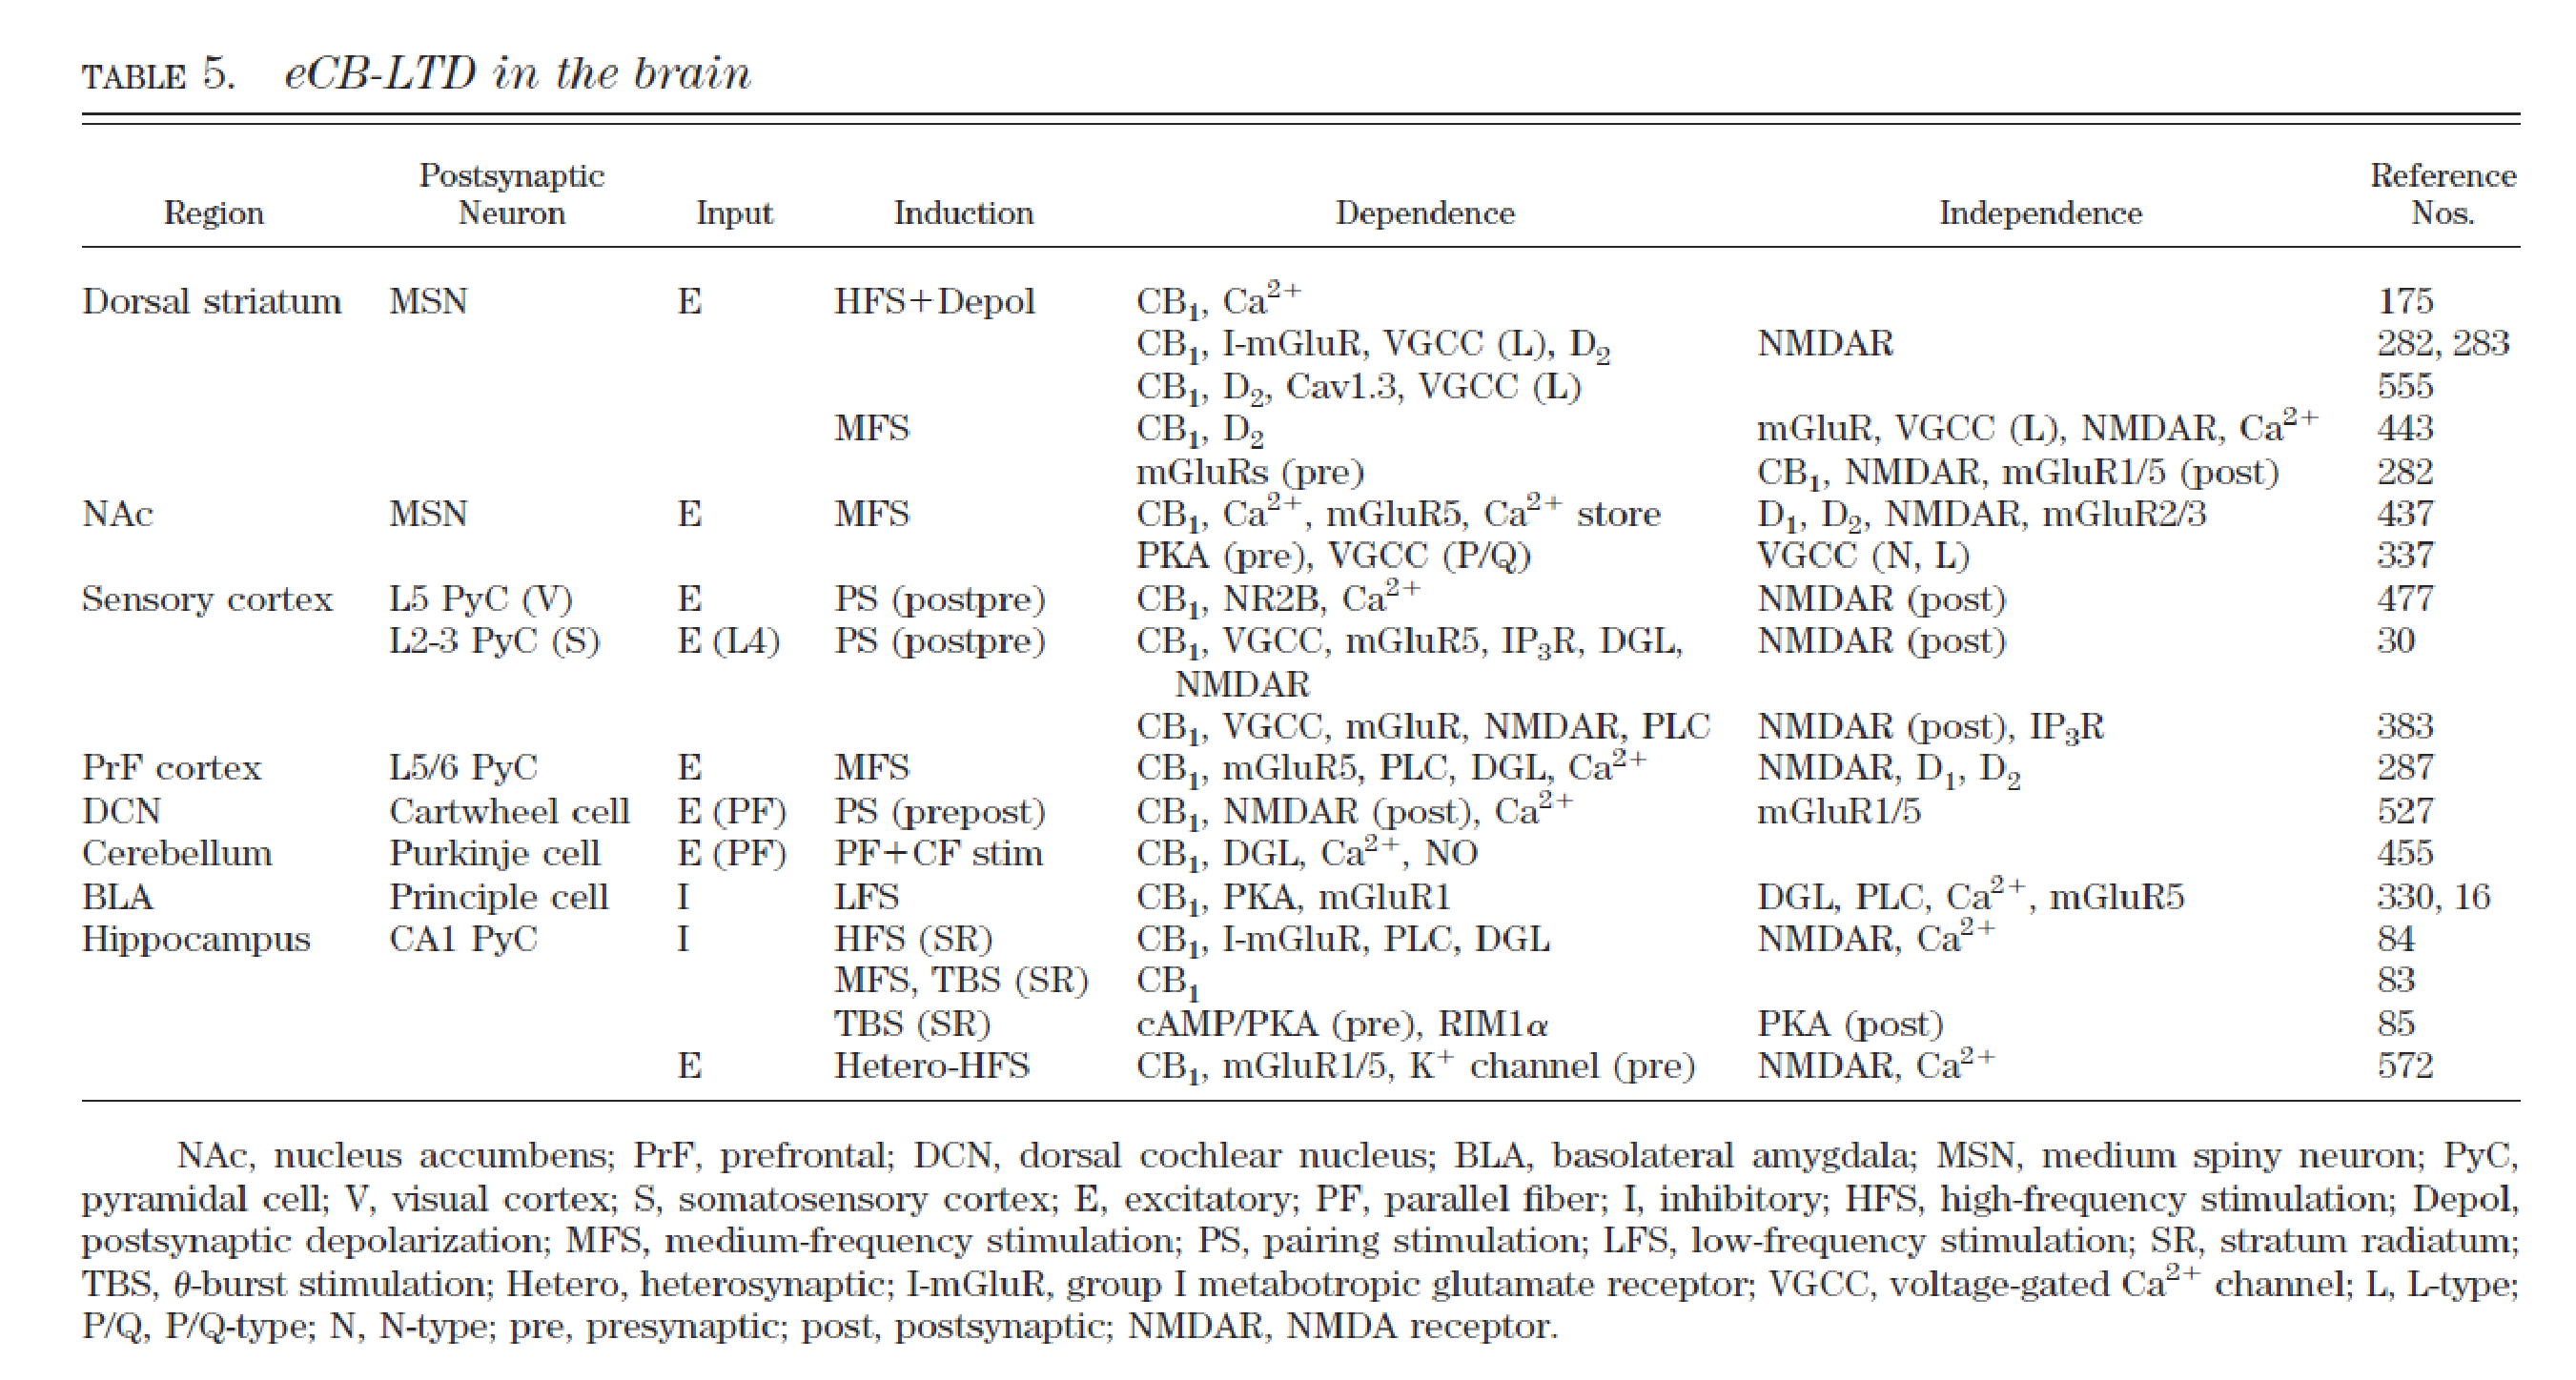
\includegraphics[height=5cm,
    angle=0]{./images/eCB-LTD.eps}}
\caption{eCB-LTD in (1) dorsal striatum; (2) NAc; (3) sensory cortex; (4)
prefrontal cortex; (5) dorsal cochlear nucleus (DCN); (6) cerebellum; (7)
basolateral amygdala; (8) hippocampus}
\label{fig:eCB-LTD}
\end{figure}

\subsection{----- corticalstriatal synapses}


The striatal LTD, which is induced by high-frequency stimulation of
corticostriatal afferents, was prevented by pharmacological or genetic depletion
of CB1, indicating the involvement of endocannabinoids.




%%% Local Variables: 
%%% mode: latex
%%% TeX-master: "mainfile"
%%% End: 
\section{Sleep-dependent memory formation}
\label{sec:sleep-dependent-memory-formation}

The importance of sleep for declarative memory consolidation has gained
increasing support over the year.
Both sleep spindles (Sect.\ref{sec:spindle-wave}) and slow oscillations have
been implicated in sleep-dependent memory consolidation (Born et al. 2006).


Sleep spindles were identified by a dynamic detection algorithm
\begin{itemize}
  \item  implemented in MATLAB (2007b, the Mathworks, Natick), closely resembling one described earlier
(Ferrarelli et al. 2007).

Briefly, for each subject and for channels C3 and C4 separately, the EEG signal
was zero-phase band-pass filtered between 11 and 16 Hz with a 4th order IIR
filter, rectified, and its envelope was computed.
Next, the average envelope amplitude during spindle-containing sleep stages (2,
3, and 4) was determined. Whenever the envelope crossed an upper threshold of
3.5 times the average envelope, a potential spindle was identified. The
beginning and end of a potential spindle were marked as the time points where
the envelope fell below one-third of the upper threshold. A sleep spindle was
required to have a minimum duration of 500 msec.

For light and deep sleep separately, spindle density (spindle count per minute),
average spindle amplitude, and average spindle duration were determined.
Finally, spindle measures from C3 and C4 were averaged. Our threshold settings
were chosen to achieve optimal agreement between spindle events detected by the
algorithm and spindles visually identified by an experienced sleep scorer (WFH).


\end{itemize}

\chapter{Rate-based vs. Spike-based memory encoding}

Does the brain use a firing rate code or a spike timing code?

\url{http://journal.frontiersin.org/article/10.3389/fnsys.2015.00151/full}




\chapter{Mathematical theory of memory encoding}

The classification is a fundamental problem in that machine learning techniques
have been widely used to solve;  e.g. neural networks
(Sect.\ref{sec:ANN-articial-neuron-network}). This network can have one input
layers, zero, one or many hidden layers; and one output layers.

\begin{enumerate}
  \item a feed-forward network with zero hidden layer (i.e. only 1 input layer
  and one output layer) is the two-layer perceptron (Sect.\ref{sec:perceptron})


However, a  feedforward  network  with input  and  output  layers  but  without 
hidden  layers  seems like a 'brain' which has input layers (eyes, noses,
etc.) and output  layers  (motor  sensors,  etc.)  but  without  'central
neurons'; making such systems having no  'learning  and  cognition' 
capabilities at  all.

Minsky and Papert (1969) showed that a perceptron without having hidden  layers 
even  could  not  handle  the  simple  XOR problem.
  
  \item a feed-forward network with single hidden layer
  
The field of ANN stalled for a decade (after Minsky and Papert's paper) until
Hopfield published two  scientific papers which was the starting point of the
era of neural network modelling in 1980s
(Sect.\ref{sec:Hopfield-neural-network}).

However, an immediate dilemma in neural network research  is  that  since hidden
 layers  are  important  and necessary  conditions  of  learning,  by default 
expectation and understanding of neural network research community, hidden 
neurons  of  all  networks  need  to  be  tuned.
This led to several learning  algorithms  to  train  various  types  of neural 
networks  mainly  by  tuning  hidden  layers (Sect.\ref{sec:train-ANN}).
Traditionally, training network has based on gradient descent methods.
  
  \item a feed-forward network with many hidden layers (deep neural network,
  deep learning)
\end{enumerate}



In games like chess, a high IQ is not necessary but at least 10,000 hours of
training is vital. During the training period, small frequently occurring
patterns, will be learned. This learning process will be non-linear, e.g. slow
first and fast later for example.


Mimicking the capability of the cortical network in learning (the capability to
hold rich information about past events) and the capability to adapt in time is
very challenging. These networks that try to mimic how the neurons works is
called (artificial) {\bf neural network} (ANN) -
Sect.\ref{sec:ANN-articial-neuron-network}).


One such model that could address temporal tasks is using back-propagation
neural network learning procedure to the analysis and recognition of speech
(Elmars - Zipser, 1988) - Sect.\ref{sec:learning-sound}. 


\section{Artificial Neural Network (ANN)}
\label{sec:ANN-articial-neuron-network}

An (artificial) {\bf neural network} (ANN) is a network of interconnected
'artificial neuron' (AN - Sect.\ref{sec:artificial-neurons}) in a directed or
indirected way, which has been designed in such a way that can mimics the
'learning' capability of the brain.

There are many types of artificial neural networks (ANN), depending upon 
(1) the constitutive artificial neurons (Sect.\ref{sec:artificial-neurons}), 
(2) the way we connects them.
\footnote{\url{https://en.wikipedia.org/wiki/Types_of_artificial_neural_networks}}


Applications:
\begin{itemize}
  \item Lee, H.: Model selection for neural network classification.
Journal of classification 18(2), 227-243 (2001)
\end{itemize}

\begin{figure}[hbt]
  \centerline{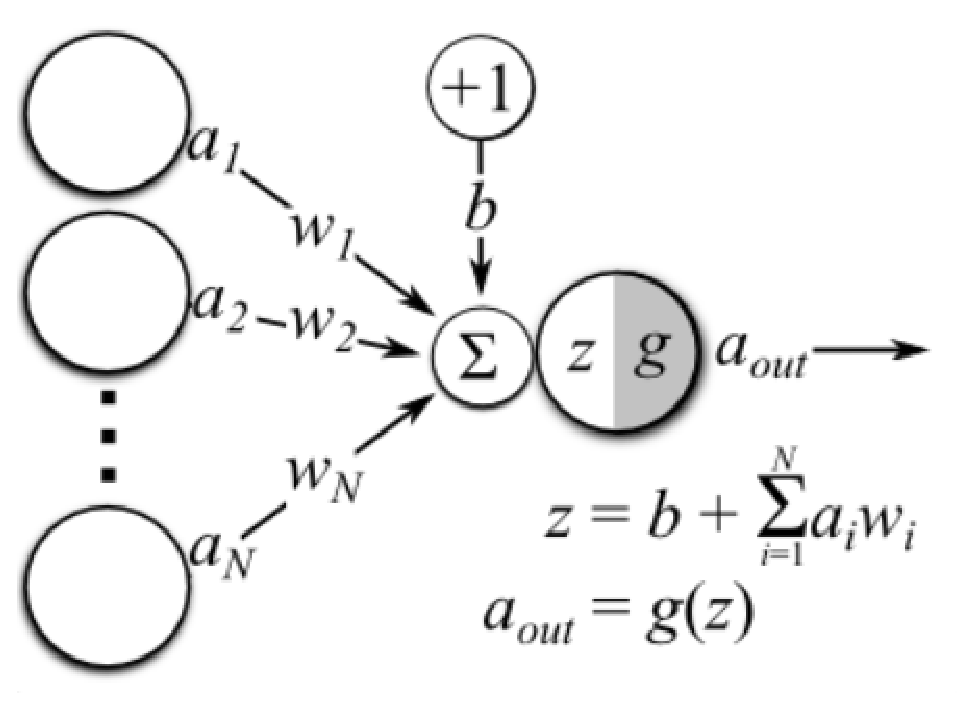
\includegraphics[height=5cm,
    angle=0]{./images/ANN.eps}}
\caption{An artificial neuron with many inputs, and 1 output}
\label{fig:ANN}
\end{figure}


\section{-- Artificial Neurons}
\label{sec:artificial-neurons}

The main problem in neural network approach is choice of activation
functions for the artificial neurons and estimation of connected weights to
obtain decision regions leading to minimum error, i.e. the learning rate.

Artificial neurons are the constitutive units of an ANN
(Sect.\ref{sec:ANN-articial-neuron-network}). Each 'artificial neuron' (AN) has
its own {\bf state} whose value depends upon its previous value, and its inputs. 
\begin{itemize}
  \item Each individual neural unit may have an activation function 
  (e.g. summation
  function) which combines the values of all its inputs together.

The artificial neuron receives one or more inputs (representing dendrites) and
sums them to produce an output (representing a neuron's axon).

Usually the sums of each node are weighted, and the sum is passed through a {\bf
non-linear function} known as an {\bf activation function} or {\bf transfer
function} (Sect.\ref{sec:transfer-function}).

  \item   There may be a threshold function or limiting function on each
  connection and on the unit itself such that it must surpass it before it can
  propagate to other neurons.  
  
This is to mimics the all-or-none behavior of the neuron's spike.
  
\end{itemize}

An artificial neuron is a mathematical function conceived as a model of
biological neurons. Based on Fig.\ref{fig:ANN}
\begin{itemize}
  \item $g(\cdot)$	 is a Heaviside step function: perceptron
  (Sect.\ref{sec:perceptron})
  
  \item $g(\cdot)$ is a linear function, i.e. $g(z) = z$
  
  \item $g(\cdot)$ is a sigmoidal function: with output values in the range
  (0,1)
  
This function is easier to take derivative than hyperbolic tangent function.
   
  \item $g(\cdot)$ is a hyperbolic tangent function: with output values in the
  range (-1,1)
  
\end{itemize}



The transfer function $\psi(\cdot)$
\begin{equation}
y_k = \psi \left( \sum_{j=0}{m} w_{kj} x_{j} \right)
\end{equation}

\begin{enumerate}
  \item the input vector $w_{kj}x_{j}$ represents the input at a single
  DENDRITIC CONTACT, e.g. synapse. 
  
  Here, it's assumed that each dendrite is able to perform "multiplication" by
  that dendrite's "weight value."
  
  \item the linear sum represents the way SOMA adds up input signal
  
  \item the non-linear $\psi(\cdot)$ represent the way AXON 'fire'the signal.
  However, in a biological neuron, the signal is fire as a all-or-none behavior,
  i.e. discrete; while most ANN uses a contiguous function which makes 
  derivative available for training the network, i.e. adjustment the weights.
  
 Using sigmoidal function, the  artificial neurons can output distinct
 values (often from -1 to 1).

\end{enumerate}

\subsection{Transfer functions}
\label{sec:transfer-function}

The transfer functions $\psi(\cdot)$ that represent the output (i.e. axon's
signal) of an artificial neuron (Sect.\ref{sec:artificial-neurons}) are often
chosen to be monotonically increasing, continuous, differentiable and bounded.

\begin{itemize}
  \item (usually) a sigmoid shape function
  
  \item (other forms): of  other non-linear functions, piecewise linear
  functions, or step functions. 
\end{itemize}

Initially, it employed a threshold function, equivalent to using the Heaviside
step function. 
\begin{itemize}
  \item if the sum > some threshold (e.g. 0), then the neuron output (e.g. 1),
  otherwise deactivated value (e.g. -1). The artificial neuron using this
  transfer function is called {\bf linear threshold units}

\end{itemize}

\textcolor{red}{The choice of non-linear transfer function is preferred. This is
because multiple layers of linear computations can be equally formulated as a
single layer of linear computations. Thus using linear activations for the
hidden layers doesn't buy us much.} IMPORTANT: using linear activations for the
output unit activation function (in conjunction with nonlinear activations for
the hidden units) allows the network to perform nonlinear regression.


In the late 1980s, when research on neural networks regained strength, neurons
with more continuous shapes started to be considered. The possibility of
differentiating the activation function allows the direct use of the gradient
descent and other optimization algorithms for the adjustment of the weights.

\subsection{binary neuron (linear threshold unit)}
\label{sec:binary-neuron}
\label{sec:linear-threshold-unit}
\label{sec:Heavyside-step-function}

The linear threshold unit computes its net input as the weighted sum of all
inputs converging to it. 

A linear threshold unit employs the threshold transfer function
(Sect.\ref{sec:transfer-function}). For a fixed threshold \verb!th!, if weighted
sum of inputs $\sum w_i$
\begin{enumerate}
  \item $> $th: output is 1
  \item $<$ th: output is 0
\end{enumerate}

An ANN that employs these neurons is the perceptron (Sect.\ref{sec:perceptron}).
However, typically the values +1 and -1 are used as output.

Based on Hebb's idea, Rosenblatt [1959] deviced automatic learning methods for
linear threshold units. More importantly, Rosenblatt provided mathematical
proofs that these methods would, under certain conditions, converge to adequate
solutions in finite time. McCulloch and Pitts's linear threshold units that are
capable of learning are essentially Rosenblatt's perceptron.

\subsection{logistic function (sigmoidal function)}

This function is very commonly used in feed-forward network
(Sect.\ref{sec:feed-forward-network}).


The derivative is
\begin{verbatim}
g'(z) = g(z) * ( 1 - g(z))
\end{verbatim}

\subsection{semi-linear unit}
\label{sec:semi-linear-unit}


\subsection{hyperbolic tangent function}
\label{sec:hyperbolic-tangent-function}


The derivative is
\begin{verbatim}
g'(z) = 1 = g(z)^2
\end{verbatim}



\subsection{radial basis function}
\label{sec:radial-basis-function}



\subsection{Nv neuron}

\subsection{McCulloch-Pitts (MCP) neuron}


\subsection{ReLU (rectified linear activation functions)}
\label{sec:rectified-linear-activation-function}

\begin{equation}
g(z) = max(0, z)
\end{equation}

This is also known as a ramp function, and it is analogous to half-wave
rectification in electrical engineering. 

This activation function has been argued to be more biologically plausible than
the widely used logistic sigmoid (which is inspired by probability theory; see
logistic regression). The rectifier is, as of 2015, the most popular activation
function for deep neural networks (Sect.\ref{sec:deep-neural-network}).
Rectifier units perform better empirically compared to sigmoid artificial
neurons and happen to be more biologically plausible than sigmoid neurons. Their
increased adoption in deep learning is based more on empirical observations than
biological plausibility.

The rectifier itself is nonlinear (its shape is like this: \verb!_/!), so the
combination of rectifier units will  therefore be nonlinear too.


An artificial neuron (i.e. unit) employing the rectifier is also called a
rectified linear unit (ReLU).
The use of this simple function allow for faster and effective training of deep
neural architectures on large and complex datasets.


\subsection{softrect / softplus function}
\label{sec:softrect}
\label{sec:softplus}

softrect/softplus function is an analytic approximation to the ReLU. A smooth approximation to the rectifier is the analytic
function
\begin{equation}
g(z) = \ln (1 + e^z)
\end{equation}
or in general
\begin{equation}
g(z) = \frac{1}{k} \ln (1 + k \times e^z)
\end{equation}
where $k$ is a hyperparameter that controls the smoothness of the rectification
around zero.

(in MATLAB-ish syntax)
\begin{verbatim}
g(z) = 1/k.*log(1 + exp(k*z))
g'(z) = 1./(1 + exp(-k*z)),
\end{verbatim}

NOTE:  The derivative of a softplus is a logistic function.





\section{Training}
\label{sec:train-ANN}

Like a baby growing to an adult, learning (or training) is necessary before the
ANN (Sect.\ref{sec:ANN-articial-neuron-network}) can be used. There are two
types of learning
\begin{enumerate}
  \item supervised - Sect.\ref{sec:ANN-supervised}
   
If instances in a dataset are given with known labels (the corresponding correct
outputs) then the learning is called supervised; in contrast to unsupervised
learning, where instances are unlabeled.

   
  \item unsupervised - Sect.\ref{sec:ANN-unsupervised}
 \begin{itemize}
   \item clustering: hope to discover unknown, but useful, classes of items
   (Jain et al., 1999).

   \item 
 \end{itemize}
\end{enumerate}

The important questions to answer
\begin{enumerate}
  \item what is the fastest algorithms to use
  
  \item do we really need to have different learning algorithms and/or to have
  different types of neural networks to achieve
   good learning capabilities of feature learning, clustering, regression and
   classification.
  
  what is the theortical explaination behind having different learning
  algorithms   and possibly manually  tuning  parameters for different  neural
  networks  and  applications
  
  \item Why   are   biological   brains   more   'efficient'   and 'intelligent'
  than  those  machines/computers  embedded with artificially designed
  learning algorithms? 
  
  \item 

\end{enumerate}

\subsection{back propagation}
\label{sec:back-propagation}

Back propagation is the technique used to train an ANN.

For a given input with known output, the error is calculated (output values are
compared with the correct answer to compute the value of some predefined
error-function), and then the error is fed back through the network.
To adjust weights properly, one applies a general method for non-linear
optimization that is called {\bf gradient descent}, i.e.
the weights are then changed such that the error decreases if the gradient of
the error function with respect to the network weights (which is indeed the
activation function) going downhill. For this reason, back-propagation can only
be applied on networks with differentiable activation functions.

For the training sets: $D = \left\{  (x_1,d_1) \ldots (x_s, d_s) \right\}$, with
$d_i$ is the desired output of the input $x_i$.

Initial values: the weights $\mathbf{w} = (w_1, \ldots, w_i, \ldots, w_m)$ of
$m$ artificial vectors (for 1 layer).

GOAL: train the values of $\mathbf{w}$, i.e. find $w_i(t)$ as the weight at time
$t$. While feeding the inputs with known output, we try to revise the values of
weights; with a given learning rate $\alpha$ ($0 < \alpha < 1$). 

\begin{equation}
w_i(t+1) = w_i(t) + \alpha (d_j - y_j(t))  x_{j,i}
\end{equation}

For off-line learning (i.e. the whole training sets are available), then we keep
feeding input data until the error 
\begin{equation}
\frac{1}{s}\sum_{j=1}^s |d_j - y_j(t)|
\end{equation}
passes a certain threshold (or a predetermined number of iterations
have been completed.)

NOTE: Too high a learning rate makes the ANN periodically oscillate around the
solution unless additional steps are taken.

\url{https://theclevermachine.wordpress.com/2014/09/11/a-gentle-introduction-to-artificial-neural-networks/}

\subsection{delta rule}
\label{sec:delta-rule}

Alternatively to back propagation, methods such as the delta rule can be used if
the function is non-linear and differentiable, although the one below will work
as well. It is a special case of back propagation algorithm
(Sect.\ref{sec:back-propagation})

It is a gradient descent learning rule for updating the weights of the inputs
in a single-(hidden) layer ANN.

\begin{equation}
w_i(t+1) = w_i(t) + \alpha (d_j - y_j(t))  x_{j,i} \times g'(h_j)
\end{equation}

with $g'(h_j)$ is the neuron transfer function, and $h_j$ is the weighted sum of
the neuron's input: $h_j = \sum x_i w_{j,i}$; and $y_j = g(h_j)$.

The error function
\begin{equation}
\frac{1}{s}\sum_{j=1}^s (d_j - y_j(t))^2
\end{equation}
NOTE: The squared error is not chosen arbitrarily, but has a number of
theoretical benefits and considerations.
\url{https://theclevermachine.wordpress.com/2012/02/13/cutting-your-losses-loss-functions-predominance-of-sum-of-squares/}



NOTE: The perceptron uses the Heaviside step function
(Sect.\ref{sec:Heavyside-step-function}) as the activation function g(h), and
that means that g'(h) does not exist at zero, and is equal to zero elsewhere,
which makes the direct application of the delta rule impossible.
 
\url{https://en.wikipedia.org/wiki/Delta_rule}

\section{-- Supervised ANN}
\label{sec:ANN-supervised}

One primary limitation of many ANNs is that they are supervised algorithms,
requiring a known target output value for each input observation in order to
train the network. This can be prohibitive for training large networks that may
require lots of training data to adequately adjust the parameters.

There are two types of supervised training
\begin{enumerate}
  \item batch training, i.e. all training data needs to be readily available
  
  \item incremental training, i.e. the parameters of the ANN can be adjusted
  once new training data become available.
\end{enumerate}

Traditionally, training network has based on gradient descent methods

\subsection{unorganized machine (Turing's machine 1948): A-type machine}


An {\bf unorganized machine} is a concept mentioned in a 1948 report by Alan
Turing. It is a machine in which its {\bf NAND gates} are largely random in its
initial construction, but capable of being trained to perform particular tasks.

Turing claimed that these were the simplest possible model of the nervous
system.
\begin{enumerate}
  \item {\bf A-type machine} (or network): build up from N 'artificial neuron',
  with an artificial neuron is a NAND gate (i.e. accepts 2 input and has 1
  output), and all the NAND gates are essentially randomly connected.

\begin{verbatim}
NAND gate
 INPUT 1         INPUT 2      OUTPUT
   1               1           0
   1               0           1
   0               1           1
   0               0           1
\end{verbatim}
They are very early examples of randomly connected, binary neural networks.
A subset I of these artificial neurons served as {\bf input nodes}, i.e.
leaving (N-I) neurons as 'processing nodes'. Each neuron, except the input
nodes, received input from {\bf exactly 2 other neurons} (as it's a neuron is a
NAND gate), so the \textcolor{red}{Number of A-type machine interconnections is}
$2\times(N-I)$.
  
  \item {\bf B-type machine} (or network): an 'artificial neuron' 
  is a three-node A-type network. 
\begin{verbatim}
A-type machine ----[connection-modifier]----> A-type
\end{verbatim}
A connection-modifier has two training fibres (red fiber and green fiber).
The purpose of having the connection-modifier is to decide when the output from
pre-node can reach the post-node. 

\begin{itemize}
  \item pass-mode:

Applying a pulse to the green training fibre sets the box to pass its
input--either 0 or 1--straight out again. This is pass mode. In pass mode, the
box's output is identical to its input. 
  
  \item interrupt mode: 

The effect of a pulse on the red fibre is to place the modifier in interrupt
mode. In this mode, the output of the box is always 1, no matter what its input. 
% While it is in interrupt mode, the modifier destroys all information attempting
% to pass along the connection to which it is attached. 

\end{itemize}
Once set, a connection-modifier will maintain its function unless it receives a
pulse on the other training fibre. The presence of these modifiers enables a B-type
unorganised machine to be trained, by means of what Turing called 'appropriate
interference, mimicking education'.


The connection modifier is itself made from A-type nodes (i.e. accepts 2
inputs).
Again, there is $2*(N-I)$ three-node A-type networks in a B-type network. A
B-type network has $14\times(N-I)$ interconnections.

SUMMARY: B-type network is constructed by replacing each interconnection in an
A-type network by a three-node switch. This connection modifier is important in
modifying the affect of one gate to
 another, and is important for 'training' the system. Before the term genetic
 algorithm was coined, Turing even proposed the use of what he called a
 genetical search to configure his unorganized machines.

 B-type machine was based on the hypothesis of learning in the brain based on
 the mechanism of neural plasticity (Sect.\ref{sec:Hebbian-plasticity})

NOTE: A D flip-flop with its preceding NAND gate is called {\bf primitive node}.

Turing claimed that the behaviour of B-type machines could be very complex when
the number of nodes in the network was large.

  \item {\bf BI-type machine}
  
  \item {\bf TB-type machine}
  
  \item {\bf TBI-type machine}
  
An N neurons TB-type or TBI-type network is built up from $N+8(N-I)$ = 
$9N-8I$ primitive nodes; and contains $18\times (N-I)$ interconnections. 

  \item  {\bf CP-type machine}
  
  \item {\bf BS-type machine} 
  
  \item {\bf B|1-type machine}
  
  
\end{enumerate}

In Turing networks, the number of interconnections is linearly dependent on the
number of neurons; so simulation and implementation of this type of network will
not suffer from 'exponential explosion'.

At Turing's time, he only used paper and pencil, as there was no computer
available. It was not until 1954, the year of Turing's death, that B.G. Farley
and W.A. Clark succeeded in running the first computer simulation of a small
neural network, at MIT; and they called it {\bf calculators}.

\subsection{perceptron (single-layer + multiple layer perceptron)}
\label{sec:perceptron}

Perceptron is a single layer neural network and a multi-layer perceptron is
called Neural Networks (Sect.\ref{sec:perceptron})


\textcolor{red}{XOR problem}: The perceptron can only produce AND or OR
operator; but not XOR. In 1973, (three years after the book in 1969 of
perceptrons by Minsky and Papert) Stephen Grossberg published a series of papers
introducing networks capable of modelling differential, contrast-enhancing and
XOR functions.


This led to the field of neural network research stagnating for many years, before it was
recognised that a feedforward neural network with two or more layers (also
called a multilayer perceptron) had far greater processing power than
perceptrons with one layer

\subsection{-- single-layer perceptron}
 
{\bf single-layer perceptron} is one of the first ANN with single layer of
articial neurons and using linear functions $\psi(\cdot)$ with a set of weights
(Sect.\ref{sec:binary-neuron}).

Most perceptrons using artificial neurons with threshold function, and have
outputs of 1 or -1 with a threshold of 0; as there is some evidence that such
networks can be trained more quickly than networks created from nodes with
different activation and deactivation values.
  
HARDWARE PERCEPTRON: It was intended as a machine, with OR, and AND operator,
making it's super fast.

\textcolor{red}{XOR problem}: The perceptron can only produce AND or OR
operator; but not XOR. In 1973, (three years after the book in 1969 of
perceptrons by Minsky and Papert) Stephen Grossberg published a series of papers
introducing networks capable of modelling differential, contrast-enhancing and
XOR functions.

In order to solve the problem, we need to introduce a new layer into our neural
networks. This layer, often called the 'hidden layer', allows the network to
create and maintain internal representations of the input
(Sect.\ref{sec:feed-forward-network}).


\subsection{perceptron (Frank Rosenblatt's multilayer perceptrons 1959)}
\label{sec:perceptron}

In the late ’50s, a Cornell scientist named Frank Rosenblatt had proposed the
world’s first neural network machine. It was called the Perceptron, and it had a
simple objective - to recognize images.

The Perceptron ran on an IBM mainframe, and it was ugly. A riot of
criss-crossing silver wires, it looked like someone had glued the guts of a
furnace filter to a fridge door. Still, the device sparked some serious sci-fi
hyperbole. In 1958, the New York Times published a prediction that it would be
the first device to think like the human brain. “[The Perceptron] will be able
to walk, talk, see, write, reproduce itself and be conscious of its existence.”

Although the perceptron initially seemed promising, it was quickly proved that
perceptrons could not be trained to recognise many classes of patterns, i.e. it
is only capable of learning linearly separable problems.


Frank Rosenblatt (1958) created the perceptron - a multilayer 'feed-forward'
networks.  It is an algorithm for pattern recognition based on a two-layer
computer learning network using simple addition and subtraction.
Frank  Rosenblatt  believes  that  multilayer  feedforward   networks
(perceptrons)   can   enable   computers   to ``walk, talk, see, write,
reproduce itself and be conscious of its existence.''  
% Rosenblatt  F.  The  perceptron:  a  probabilistic  model  for  infor-
% mation  storage  and  organization  in  the  brain.  Psychol  Rev.
% 1958;65(6):386-408.

Minsky and Papert  (1969) do not believe that perceptrons  have  such  learning
capabilities  by  giving  a counter example showing that a perceptron without
having hidden  layers  even could  not  handle  the  simple  XOR problem.
In many cases, a feedforward network with input and output layers but without
hidden layers is considered as a two-layer perceptron, which were actually used
in Minsky and  Papert

Such a counter example made many researchers run  away  from  artificial  neural
networks  and  finally  re- sulted in the 'Artificial Intelligence (AI) winter'
in 1970s.
% Minsky  M,  Papert  S.  Perceptrons:  an  introduction  to  computa- tional
% geometry. Cambridge: MIT Press; 1969

\subsection{Radial Basis Function (RBF) networks: traditional three layer,
feed-forward model trained with back propagation}
\label{sec:RBF-network}

Radial Basis Function (RBF) networks consist of one hidden layer with radial
basis activation functions (Sect.\ref{sec:radial-basis-function})


\section{-- Unsupervised ANN}
\label{sec:ANN-unsupervised}

% However, there are a set of unsupervised variants of ANNs that can be used to
% learn an initial condition for the ANN (rather than from randomly-generated
% initial weights) without the need of target values
% (Sect.\ref{sec:ANN-unsupervised}).

There are a set of unsupervised variants of ANNs that can be used to learn an
initial condition for the ANN (rather than from randomly-generated initial
weights) without the need of target values.

This technique of "unsupervised pretraining" has been an important component of
many "deep learning" models used in AI and machine learning. 

\subsection{NOTE: symbolic system vs. ANN}

One of the strengths of neural networks that makes them different from symbolic
networks is that the rules (i.e. the weights) for the manipulation of the input
symbols are 'learned', not pre-loaded into the system.

However, this solution relies on a certain network architecture, and that
architecture is pre-defined, just like the rules of a symbolic system.

The question is if we can have a neural network system that can change its
architecture depending on the outputs that the network creates.

\subsection{feed-forward network}
\label{sec:feed-forward-network}

A general feed-forward network pass the input through one or many transformation

\begin{equation}
\begin{split}
a_k &= g_k \left( z_k \right) \\
    &= g_k \left(b_k + \sum_j (a_{j} w_{j,k}) \right) \\
    &= g_k \left(b_k + \sum_j (g_{j}\left( b_j + \sum_i (a_{i} w_{i,j}) \right)
    w_{j,k}) \right)
\end{split}
\end{equation}
NOTE: $a_{j}$ is the output of a neuron in layer $j$-th.

\subsection{-- original feed-forward network}

A few change in the feed-forward network compared to the perceptron
\begin{enumerate}
  \item  each connection to have a weight that is not just '1' or '-1'.
  
  \item we drop the 'threshold' for each node, and add a 'bias'. 
  
\begin{verbatim}
SUM(wjxj) + bias = threshold
\end{verbatim}
The bias and the threshold really serve the same purpose.
However, being on opposite sides of the equation, though, they are "negatively
proportional".

  \item without a threshold, we have to change the function that activates
  the network. We change the rule for activation to the following:

Activation is equal to 
\begin{equation}
f(\cdot) = \frac{1}{1- \exp^{-\sum(w_{kj}x_j)+\text{bias}}}
\end{equation}
which is a logistic function (Sect.\ref{sec:logistic-function}).
%1 over 1 minus e raised to the power of the negative sum of the net input to
% the node and that node's bias.
\end{enumerate}

{\bf feedforward neural network}: two or more layers connected in a
  feed-forward way, i.e. each neuron in one layer has directed connections to
  the neurons of the subsequent layer. In many applications the units of these
  networks apply a {\bf sigmoid function} as an activation (transfer) function.
The sigmoidal function has a continuous derivative, which allows it to be
used in back propagation (Sect.\ref{sec:back-propagation}). This function is
also preferred because its derivative is easily calculated:
\begin{equation}
f' = f * (1-f)
\end{equation}

\subsection{-- single hidden layer}

Using logistic function as transfer function, the single-layer network is
identical to the logistic regression model, widely used in statistical modeling. 
  
To train the network, i.e. the weights, multi-layer networks use a variety of
learning techniques (Sect.\ref{sec:train-ANN}), the most popular being {\bf
back-propagation} (Sect.\ref{sec:back-propagation}).

\subsection{-- bias and threshold}

\url{http://stackoverflow.com/questions/6554792/whats-the-point-of-the-threshold-in-a-perceptron}

\subsection{-- the curse of dimensionality}

Biological networks are sprawling, randomly interconnected things. They are very
irregular and vicarious. In contrast, an ANN is pretty rigid in structure, in
terms of what layers it has and how they are connected.

While traditional multilayer perceptron (MLP) models were successfully used for
image recognition, due to the full connectivity between nodes they suffer from
the curse of dimensionality and thus do not scale well to higher resolution
images.


\subsection{-- convolution neural network (CNN): LeNet-5}
\label{sec:LeNet-5}
\label{sec:CNN}


CNN (ConvNet) is a type of feed-forward ANN in which the connectivity pattern
between its neurons is inspired by the organization of the animal visual cortex,
whose individual neurons are arranged in such a way that they respond to
overlapping regions tiling the visual field.

The predecessor to CNN is neocognition (introduced in 1980).
The neocognitron differs from convolutional networks because it does not force
units located at several positions to have the same trainable weights.

Convolutional Neural Networks are designed to recognize visual patterns directly
from pixel images with minimal preprocessing.
The famous LeNet-5 network (i.e. 5 layers) can classify digits successfully and
is applied to recognising hand-written check (cheque) numbers.
\url{http://yann.lecun.com/exdb/lenet/}

A CNN architecture is formed by a stack of distinct layers that transform the
input volume into an output volume (e.g. holding the class scores) through a
differentiable function. A few distinct types of layers are commonly used

\subsection{ReLU ANN}

An artificial neuron in a ReLU ANN is called ReLU.
ReLU uses rectified linear activation functions
(Sect.\ref{sec:rectified-linear-activation-function}).
They exhibit some nice invariance properties that are useful for pattern
recognition.

Check Bengio's group on rectifier nets.

\subsection{Linear neuron vs. Nonlinear neuron}
\label{sec:linear-neuron}
\label{sec:nonlinear-neuron}

In linear neuron, the output of a neuron $j$-th is the weighted sum of all
$n$ inputs:
% \[ 
% y_j = \sum_k w_{kj} x_{kj} 
% \]
% the weighted sum of the input
\begin{equation}
y_j = \sum_{k=1}^n w_{kj}x_{kj}
\end{equation}

% \[ 
% y_j = \sum_i w_{ij}x_i
% \] 
or $\mathbf{y}=\mathbf{w.x}$.

Fig.\ref{fig:artificial-neuron} shows a connection between two artificial
neurons with the connection function can be linear or nonlinear.

\begin{figure}[htb]
  \centerline{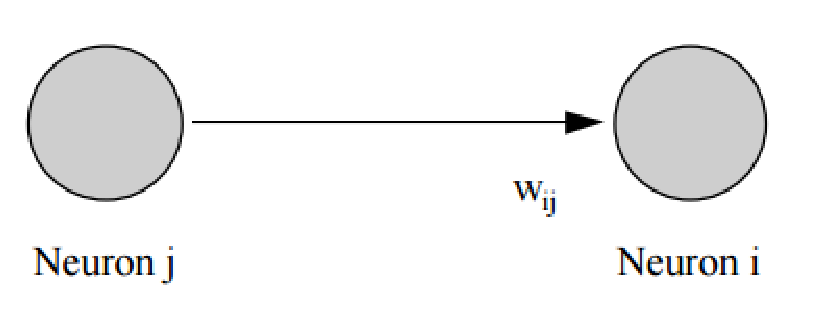
\includegraphics[height=2cm]{./images/Hebbian_simple_formula.eps}}
  \caption{Synaptic weight $w_{ij}$:
  $y_i=F[w_{ji}x_j]$ with $F[\cdot]$ is some
  linear or non-linear function transforming the input into output activity}\label{fig:artificial-neuron}
\end{figure}


\subsection{Synaptic plasticity in ANN}
\label{sec:synaptic_plasticity-ANN}


The {\bf synaptic weight} refers to the {\bf strength} or {\bf amplitude} of a
connection between the presynaptic side and postsynaptic side,
Fig.\ref{fig:artificial-neuron}.
It represents the amount of influence the firing of one neuron has on another.

\begin{figure}[hbt]
  \centerline{
  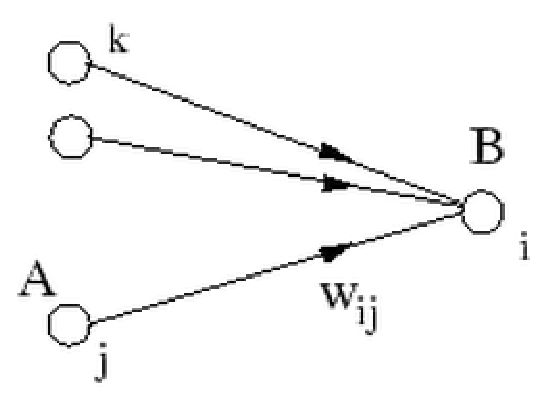
\includegraphics[height=4cm,
    angle=0]{./images/synaptic_plasticity_efficacy.eps}}
\caption{Synaptic weight in artificial neurons represents synaptic plasticity
efficacy in real neurons}
\label{fig:synaptic_plasticity_efficacy}
\end{figure}

We will investigate two cases:
\begin{itemize}
  \item a single neuron receiving multiple inputs, Fig.\ref{fig:synaptic_plasticity_efficacy}
  \item a single layer of multiple neurons, all receiving the same set of inputs
\end{itemize}

The synaptic weight $w_{ij}$ represent the connection strength from presynaptic
neuron $i$ to postsynaptic neuron $j$, the presynaptic signal is the input
$x_i$, and the postsynaptic neuron output is $y_j$. A linear neuron is often
assumed (Sect.\ref{sec:linear-neuron}).

Historically, it was thought that the synaptic weights $w_{ij}$ of these
connections, once established during development, were relatively fixed in their
strength, much like a solder joint between two electronic components.
Interestingly, this is not true, i.e. \textcolor{red}{most synapses are
extremely plastic}, i.e. they are able to change their strength as a result of
either their own activity or through activity in another pathway.

In neuroscience, {\bf synaptic plasticity} is the ability of synapses
(Sect.\ref{sec:synapse}) to strengthen or weaken over time, in response to
increases or decreases in their activity. 
\textcolor{red}{Many think that this synaptic plasticity is central to
understanding the mechanisms of learning and memory}.
The synaptic weight is changed, i.e. $\Delta w_{ij}$, by using a learning rule.

The first learning rule is Hebbian learning rule: -
Sect.\ref{sec:Hebbian_learning}. At a positive learning rate $\eta$, 
the weight keeps increasing over time, i.e unstable. 

The strategy for constraints:
\begin{itemize}
  \item keep the sum of weights constant: Sect.\ref{sec:Oja-learning-rule}
  
  \item use the postsynaptic activity to adjust the threshold for potentiation

  \item regulate neuronal excitability
  
  \item scale all of a neuron's synaptic weights
\end{itemize}
All these mechanisms stabilize postsynaptic activity and introduce
competition, but the choice of constraint influences strongly the
behavior of the model.



\section{Regression vs. Classification)}

\begin{itemize}
  \item  Regression: the output variable takes continuous values.

Regression involves estimating or predicting a response. 

 \item Classification: the output variable takes class labels.

Classification is identifying group membership.  
\end{itemize}


In some cases of classification we can consider probabilistic models (eg
logistic regression) where each class or label has some probability which can be
weighted by the cost associated with each label or class and thus give us with
final value on basis of which we can decide to put it some label or not.
(for example: label A has probability of 0.3 but the payoff is huge (1000)
however label B has probability 0.7 but the payoff is very low 10.So for
maximizing the profit we might label the example as label A instead of B.


\section{Linear regression vs. Non-linear regression}





\section{Learning 'sound'}
\label{sec:learning-sound}

In a system developed by Elmars-Zipser (1987) using back-propagation neural
network, there is no given description of speech features; instead the system
'learnt' from the training input-output pairs to develop its own set of
representational features, and it gaves 95\% of accuracy.
% Learning the Hidden Structure of Speech




\section{Two-stage theory}
\label{sec:two-stage-theory}
\label{sec:austin-simonson-theory}

\section{Theory of Encoding Specificity}
\label{sec:theory-of-encoding-specificity}

\section{Memory learning}
\label{sec:memory-learning}

Check Klein, Shapiro, Kandel (1980) as starting point. 

\section{Learning rule}
\label{sec:learning-rule}

Learning rule refers to the the 'rule' defined for increasing/reducing the
'weight' (or synaptic plasticity) between connected neurons. While the
underlying cellular  mechanism is still not clearly understood; there have been
different 'mathematical formula' developed for controlling these (synaptic)
weights. To explain the different forms of memory in the brain, different forms
of learning mechanism have also been proposed.

\subsection{Hebbian learning (associative learning + competitive learning)}
\label{sec:Hebbian_learning}

As discussed in the earlier text, Hebb (1949) proposed a mechanism to explain
when the synaptic conductance is increased. The idea that connections between
neurons that are active {\bf at the same time} are strengthened is often
referred to as "Hebbian learning" (Sect.\ref{sec:Hebbian-synapse}).

\textcolor{red}{Remember that ``at the same time'' is a relative statement in
biology}, i.e. as long as they occur at a small enough time difference $\Delta
t$ they are called to occur at the same time.

The original publication of Hebb only discuss the increase in synaptic efficacy
via co-activation. This is called {\bf associative learning} or {\bf
Hebbian learning}. Since then, several key features have been included into the
concept of Hebbian synapse (see below).

{\bf Hebbian learning}, the development of neural circuits based on
correlated activity, relies on two critical mechanisms
\begin{enumerate}
  \item associative learning
  
  \item competitive learning
\end{enumerate}

% \subsubsection{Associative (Cooperative) learning}
\subsection{* Original Hebbian learning (associative (cooperative) learning)}
\label{sec:associative_learning}
% Because of this property, the Hebbian learning rule can serve to form {\bf
% associations} between the activity in the pre- and postsynaptic neurons
{\bf Associative learning} (the one proposed by the Canadian neuropsychologist
Donald Olding Hebb): {\it activity-dependent synaptic modification along the
lines}

%\begin{Verbatim}
% \end{Verbatim}

Depending on the region of firing, the action potential can be postsynaptic
potential (Sect.\ref{sec:synaptic_potential}).

% \begin{verbatim}
% Neurons that fire together, wire together
% \end{verbatim}
% \item 
Example:
As shown in Fig.\ref{fig:Hebbian_plasticity}, a pyramidal cell (post) is
depolarized (i.e. active) at the same time with one of its coming input is
activated (i.e. presynaptic neurons fires), after a certain time (i.e. many
times of co-activation), the recording of the potential of the pyramidal cell
increases. This increase is long-lasting, i.e. a persistent strength in
connection, and the changes to occur is slow.
The biological mechanism for this cooperative learning are explained by
NMDA-dependent {\bf Long-term potentiation} in hippocampus
(Sect.\ref{sec:long-term_potentiation}).

 
The synaptic weight $w_{ij}$ (from neuron $j$ to $i$) is modeled as
\begin{enumerate}
  \item form 1: {\bf pattern learning} which is the 
  function of the pre-synaptic inputs to the two
  neurons
\[
w_{ij} = x_i x_j
\]
assuming that each neuron has only one presynapse with $x_i$, $x_j$ are the
pre-synpaptic output for neuron $i, j$, respectively.

In Hopfield artificial neural network, $w_{ii}= 0$ (no reflexive connections
allowed).

  \item form 2: {\bf epoch learning} (the weight is updated once all the inputs
  are presented - they must be presented within a time window)
\[
w_{ij} = \frac{1}{p} \sum^p_{k=1} x_i^k x_j^k
\]
with $p$ is the number of training patterns, $x_i^k$ is the $k$-th input of the
neuron $i$.
 
   \item Harry Klopf's model:   
\end{enumerate}

\subsection{* Competitive Hebbian learning}
%\subsubsection{Competitive learning}
\label{sec:compatitive_learning}

{\bf Competitive Hebbian learning}:  a mechanism that forces different synapses
to compete with one another so that when some synapses to a given postsynaptic
neuron are strengthened, others are weakened
\citep{guillery1972, miller1996, song2000}


\begin{figure}[htbp]
  \centerline{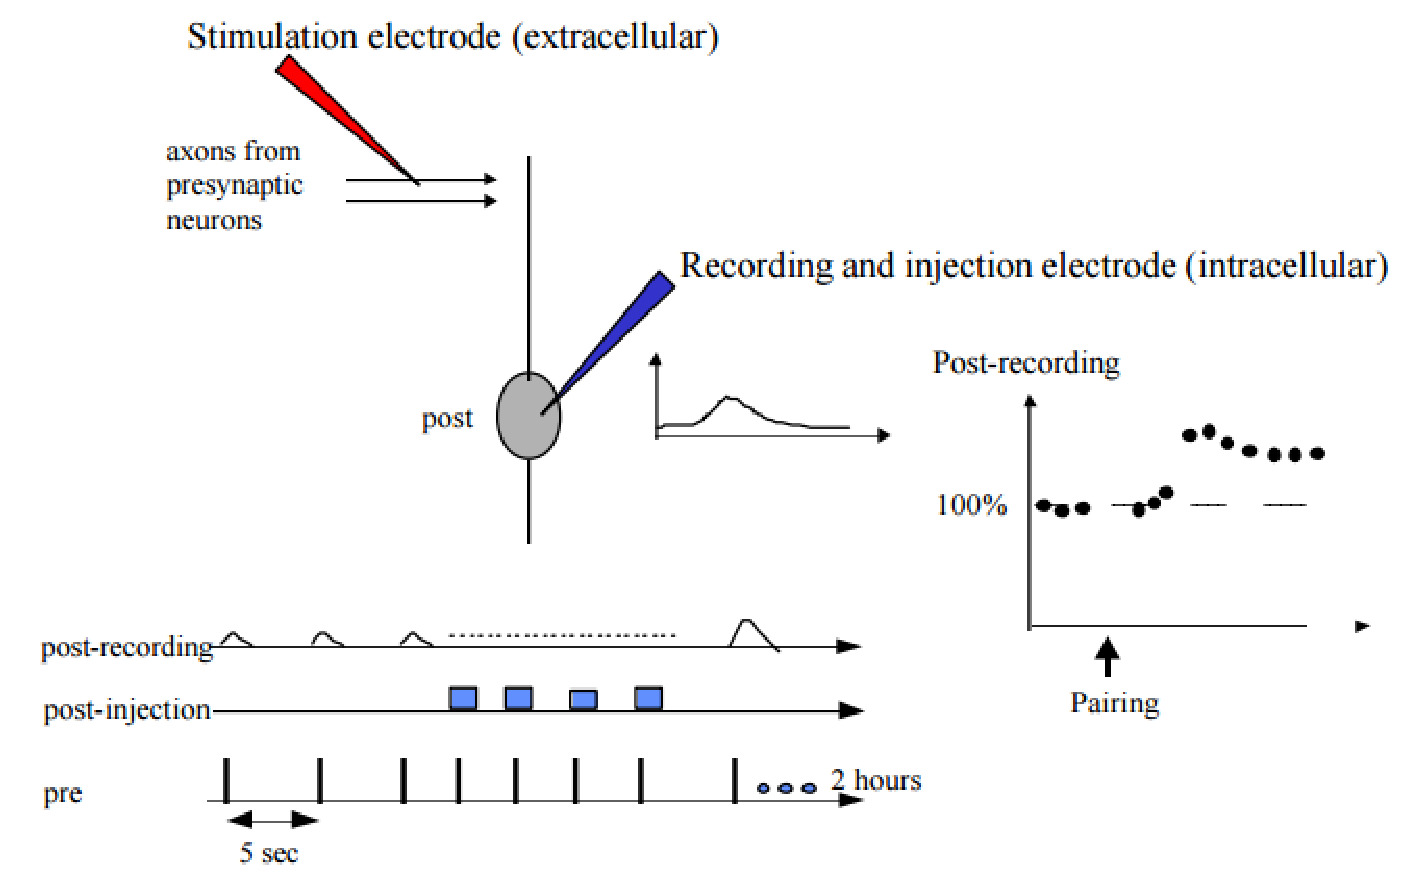
\includegraphics[height=6cm]{./images/Hebbian_plasticity.eps}}
  \caption{Hebbian plasticity (associative
  learning)}\label{fig:Hebbian_plasticity}
%http://www.nbb.cornell.edu/neurobio/linster/BioNB420/hebb.pdf
\end{figure}

Over the past several decades, Hebb's idea has been extended into various forms
of correlation-based rules for synaptic modification and successfully used in
many learning networks and in the analysis of activity driven refinement of
developing circuits
\begin{itemize}
  \item (Stent 1973, Sejnowski \& Tesauro 1989, Brown et al 1990, Fregnac \&
  Bienenstock 1998, Sejnowski 1999)
\end{itemize}



It is often assumed that long-term depression (LTD) can account for such
competition; but LTD as characterized thus far is not up to the task.


\subsection{Generalized Hebbian Learning}
\label{sec:Hebbian-generalized}

Instead of calculating the synaptic weight $w_{ij}$, the change $\Delta
w_{ij}$ is calculated. The generalized Hebbian rule is based on the idea that
change in a given synaptic weight is proportional to both the pre-synaptic input
$x_i$ and the output activity of the post-synaptic neuron $y_j$.

Here, the change in synaptic weight at synapse $i$-th from neuron $j$ is equal
to the learning rate $\eta$ times the input signal $x_i$ times the postsynaptic
neuron output $y_j$ 
\begin{equation}
\label{eq:generalized-Hebbian-learning}
\Delta w_{ij} = \eta x_i y_j 
\end{equation}
with linear neuron assumption (Sect.\ref{sec:linear-neuron}).
This clearly maps to the concept: ``neurons that fire together, wire together''.

The learning rate $\eta$ is typically small.
Due to this, one input vector (whose $i$-th component is the term $x_{ij}$) only
causes a small instantaneous change in the weights, but when the small changes
accumulate over time, the weights will settle to some values.

In Sect.\ref{sec:Hebbian_learning}, it uses $\eta=1$.%, and $w_j=1$.
For any neural model, the Hebbian learning rule is unstable, as there is nothing
stop the weights from growing all the time for a positive learing rate (finally
leading to a very large values), i.e. the synaptic weights that receives the
dominant input will increase or decrease exponentially.

%\subsection{Normalized weight Hebbian learning}
\subsection{Oja's learning rule (1982): normalized weight Hebbian learning}
\label{sec:Oja-learning-rule}

The weight is normalized to the range [0,1]
\begin{equation}
w_{ij}^{(t+1)} = \frac{w_{ij}^{(t)} + \eta y_j x_{ij}}{\left(
\sum_{k=1}^n[w_{kj} + \eta y_j x_{kj}]^p\right)^{1/p}}
\end{equation}
Oja's original paper uses $p=2$ (corresponding root sum of squares).
However, any type of normalization, even linear, will give the same result
without loss of generality.

For small learning rate $\eta \ll 1$, Taylor series is used
\begin{equation}
w_{ij}^{(t+1)} = \frac{w_{ij}^{(t)}}{\left(\sum_{k=1}^n w_{kj}^p \right)^{1/p}}
+ \eta \left( \frac{y_j x_{ij}}{\left(\sum_{k} w_{kj}^p\right)^{1/p}}
-
\frac{w_{ij}\sum_k y_j x_{kj}w_{kj}}{\left(
\sum_k w_{kj}^p\right)^{1+\frac{1}{p}}}
\right) 
+
\mathcal{O}\left(\eta^2\right)
\end{equation}
Then, for $\eta \ll 1$, the high-order term $\mathcal{O}(\eta^2)$ is removed. 

The weights normalized to zero
\begin{equation}
|w| = \left(\sum_{k=1}^n w_{kj}^p \right)^{1/p} = 1
\end{equation}
Then the equation above becomes
\begin{equation}
w_{ij}^{(t+1)} = w_{ij}^{(t)} +\eta y_j (x_{ij} - w_{ij}y_j) 
\end{equation}


{\bf Oja's learning rule} is a single-neuron $j$-th special case of generalized
Hebbian algorithm with $n$ inpus $x_1, x_2, \ldots, x_n$, each with weight
$w_{ij}$. 

Similar to Hebbian learning rule, linear neuron is assumed
(Sect.\ref{sec:linear-neuron}). However, a 'forgetting' term is added to the
formula.
The idea is that this forgetting term should proportional not only 
to the value of the weight, but also to the square of the output of the neuron
$y_j^2$.
% The presynaptic weight $w_{ij}$ from neuron $i$ to $j$
\begin{equation}
\begin{split}
\Delta w_{ij} &= \eta (y_j x_{ij} - y_j^2 w_{ij}) \\
   &=\eta y_j (x_{ij} - y_j w_{ij}) 
\end{split}
\end{equation}
with $i=1\ldots n$.
The squared output $y_j^2$ guarantees that the larger the output of the neuron
becomes, the stronger is this balancing effect.

The learning rate $\eta$ cannot be a constant but has to decrease over time. A
typical decreasing sequence is
\begin{equation}
\eta(t) = \frac{1}{t}
\end{equation}

When there are multiple neurons on the same layer, that all receive the same set
of inputs. To prevent all neurons in this layer from learning the same thing,
parallel connections between them are needed.
\url{http://www.scholarpedia.org/article/Oja_learning_rule}

The time evolution of the output of the neuron becomes the first principal
component of the data set. In a network of neurons, we can get as many principal
components as needed. This is in analogy to PCA method (principal component
analysis). 
% Here, a principal component $w_{ij}$ is extracted from a dataset
% $\mathbf{y_j}$, through some associated vector $\mathbf{x}_j$, from that the
% original dataset can be restored using
% \begin{equation}
% \mathbf{y}_j = \sum_{i} w_{ij} \mathbf{x}_j
% \end{equation} 
\url{http://en.wikipedia.org/wiki/Oja's_rule}

\textcolor{red}{There is no direct experimental evidence yet of Oja's rule
active in a biological neural network}.

\subsection{Sanger's rule (1989): Generalized Hebbian Algorithm (GHA)}
\label{sec:Sanger-rule}

It is similar to Oja's rule in its formulation and stability, except it can be
applied to networks with multiple outputs.

The name GHA originates because of the similarity between the algorithm and a
hypothesis made by Donald Hebb, i.e. changes are proportional to the
correlation between the firing of pre- and post-synaptic neurons.

GHA combines Oja's rule with the Gram-Schmidt process to give the learning rule
\begin{equation}
\Delta w_{ij} = \eta \left( 
y_jx_{ij} - y_j \sum_{k=1}^n w_{\ldots}y_k
\right)
\end{equation}

Its importance comes from the fact that learning is a single-layer proces, i.e.
that is, a synaptic weight changes only depending on the response of the inputs
and outputs of that layer, thus avoiding the multi-layer dependence associated
with the backpropagation algorithm.

\url{https://en.wikipedia.org/wiki/Generalized_Hebbian_Algorithm}

\subsection{BCM rule (1981)}
\label{sec:BCM-rule}

BCM rule (aka BCM theory, BCM synaptic modification) is named after 3
scientists: Elie Bienenstock, Leon Cooper, and Paul Munro.
The theory was proposed to explain the learning in visual cortex.

The theory proposed a sliding threshold for LTP and LTD induction
and states 
{\it that synaptic plasticity is stabilized by a dynamic adaptation of the
time-averaged postsynaptic activity}.
\begin{itemize}
  \item reducing the postsynaptic activity decreases the LTP threshold and
  increases the LTD threshold
  
  \item increase the postsynaptic activity increases the LTP threshold and
  decreases the LTD threshold
\end{itemize}


\subsection{Maximum information (informax) - Linsker}
\label{sec:informax}
\label{sec:Linsker-informax}

A linear model 'neuron' with
\begin{itemize}
  \item multivariate Gaussian input and additive Gaussian noise
\end{itemize}

\subsection{Information-maximisation (Bell-Sejnowski (1995))}
\label{sec:Information-maximisation}
\label{sec:Bell-Sejnowski-1995-information-maximisation}


\citep{bell-sejnowski-1995} developed a unifying learning theory based on
Linsker's {\it informax} principle (which was applied for linear unit -
Sect.\ref{sec:informax}) and applied to non-linear units with with arbitrarily
distributed inputs un corrupted by any known noise sources


GOAL: how to maximise the mutual information that the output Y of a neural
network processor contains about its input X. This is mapped to the
entropy-based problem
\begin{verbatim}
Information(Y,X) = H(Y) - H(Y|X)
\end{verbatim}
with H(Y) is an entropy of the output Y; and H(Y|X) is the entropy the output
has which didn't come from the input X. 

\section{Winnerless competition (WLC) - Rabinovich et al. (2001)}

Based on the hypothesis that each stimulus is characterized by a specific and
reproducible sequence of firing across specific neurons, Rabinovich et al.
proposed a model for such encoding in a network of inhibitory and
excitatory sensory neurons using a class of dynamical system called {\bf
winnerless competition} (WLC) or competitive networks \citep{rabinovich2001}. 


The stimulus in the sensory network is ordors, each is represented by a 
different spiking pattern of olfactory bulb's projection neurons
(Sect.\ref{sec:olfactory-bulb}).

Rabinovich et al. showed that regardless of the neuron's behaviors before the
onset of the stimulus, the neuron can quickly change its behavior depending upon
the different odors. This shows a winnerless strategy, i.e. a new input can
override the behavior/dynamics of the network established from a previous input.

\subsection{Networks of N neurons}

The $i$-th neuron's membrane potential at time point $t$ is represented as
$y_i^1(t)$. 

Consider a network of $N$ neurons, the change in all membrane potentials is
represented as
\begin{equation}
\frac{d\mathbf{y}_i(t)}{dt} = F[\mathbf{y}_i(t)] - \sum_{j=1}^N
G_{ij}(\mathbf{S}) \cdot \left[ \mathbf{y}_j^1(t), \mathbf{y}_i^1(t) \right]
+ \tilde{\mathbf{S}_i}(t)
\end{equation}
with 
\begin{itemize}
  \item Both $\mathbf{S}(t) = \left\{ S_i(t) \right\}$ and
  $\tilde{\mathbf{S}_i}(t)$ represent the stimuli to every neurons in the
  network ($i=1\ldots N$).

The stimuli is represented as 2 parts: 
\begin{enumerate}

  \item  the first part representing the effect of exciting a subset of
  sensory neurons through the additive $\tilde{\mathbf{S}_i}(t)$; the second
  part

  \item the second part represents the effect of modifying inhibitory effect
  from one sensory neuron to another $G_{ij}(\mathbf{S})$.
\end{enumerate}

  
  \item 
\end{itemize}

\subsection{Firing rate}

The details of neuron's membrane potential is ignored; and the system only
abstractly capture the 'firing' or 'notfiring' state of the component neurons;
which is now simplified as an equation of firing rate.

\begin{equation}
\frac{a_i(t)}{dt} = a_i(t) \left[  \sigma_i(\mathbf{S}) - \left( a_i +
\sum_{j\neq i}^{N} \rho_{ij}(\mathbf{S}) a_j(t) \right) \right]
\end{equation}

The equation is a similar form of Lotka-Volterra equation
(Sect.\ref{sec:Lotka-Volterra-equation}) in that the increasing activity of one
inhibitory neuron would decrease the activity of the other excitatory neuron
(via inhibition effect), and the decrease of this excitatory neuron will reduce
the activity of the inhibitory neuron.

\subsection{}



\section{Information Theory (Shannon)}

Shannon's seminal 1948 paper, "A Mathematical Theory of Communication,"
established a whole new discipline, Information Theory.

Basically, it shows how a digital computer (with  Boolean algebra and basic
thermodynamic principles) could be applied to communication (an analog world).
Information (from the analog world) - Shannon provided a mathematical theory for
encoding information by applying a value to it - either 0 or 1.

The applications which make contemporary digital information services possible,
from the Internet to the iPod to HDTV, applications such as data and image
compression, detection, estimation, prediction, cryptography, error-correction
coding, modulation, and networking all depend on Information Theory.

\subsection{``information'' definition}

Shannon proved that 'information' can be quantified, and demonstrated that
mathematics could be used to calculate the theoretical maximum amount of
information carried by a communications system based upon the physical laws of
thermodynamics.

This made it possible to identify the critical relationships between various
network elements.

\subsection{entropy}

A key measure in information theory is "entropy".

\subsection{-- application to digital communication}

Signal travels through a channel (which can be
\begin{itemize}
  \item  a path over an electrical wire, an optical fiber or 
  \item  (in wireless system) a tiny slice of radio spectrum used to transmit
  the message
\end{itemize}
). Often many channels share the same wired or wireless links. The question is
how many channel you can put on the same wire to be able to get it at the other
end.

Shannon's equations told engineers how much information could be transmitted
over the channels of an ideal system. When Shannon published his theory in 1948,
the largest communications cable in operation could carry up to 1,800 voice
conversations. Twenty-five years later, the highest capacity cable was carrying
230,000 simultaneous conversations.
Today a single strand of optical fiber as thin as a human hair can carry more
than 6.4 million conversations.

\url{http://www.greentouch.org/?page=shannons-law-explained}


\subsection{-- application to neural network}

Feature detector: consider the input X to a neural unit 
is the amount of evidence for a certain
feature, and Y is the probability that the feature is present.

\section{SORN: self-organizing recurrent network}
\label{sec:SORN}

SORN emerged as a limit cycle. It's hard to choose the size of the limit cycle.

It can reaches the stable limit cycle, but not stable fixed point.

The length of limit cycle, determines the 

The converge to limit cycle. 

A system can converge to a limit cycle or a fixed point.

How a system goes to limit cycle different from goes to a fixed point?

A reservoir is important as everything can be mapped to a limit cycle

Spontaneous SORN vs. Input-driven SORN.

Static reservoir means no-learning (i.e. stop STDP and the weight keeps the
same).

Example: train 'abbbb...bc'
\begin{itemize}

  \item You give 'a' at 1 given time-step, and the network obsorb that, i.e. learnt
You then give 'b' at the next time-step, and the network continue to obsorb,
i.e. learnt.

  \item when you give 'b' repeatedly, you starts 
  

  \item the state of the network should be able to predict what will be injected
  next
  
\end{itemize}

Example: aaabbbcc, then you should have 3 limit cycles


How to pick up a sequence at any point in time. 




log-normal distribution (Sect.\ref{sec:Log-normal-distribution})


Syn-fire ring 



\section{Template Theory}
\label{sec:learning_Template-Theory}

The Template Theory is a direct result of earlier work by Simon and colleagues
who had considered the role of perception in problem solving.
Simon summarized ``{\it \ldots The situation has provided a cue; this cue has
given the expert access to information stored in memory, and the information
provides the answer}''.

The environment is too complex and thus is typically difficult for our cognitive
to process using deliberative reasoning (e.g. such as Ponzo illusion that make
we think two bars are of different length) but the information contained in
localised chunks of the environment is too focused to be useful by itself.
When the contextual cues are removed the illusion vanishes. So, what we would
like to find are the small number of visual cues that make up the salient
aspects of the environment and show how these cues change as a function of skill
(Harre et al., 2012).

The visual signal is received and comes through very early processing in the
visual cortex, area V1 that reduces that vast amount of information we receive
from the environment before sending to working memory (WM-
Sect.\ref{sec:working-memory}). The WM does not expand with
task-specific training, i.e. a bottleneck. This bottleneck sets an upper limit
on how much information can be held in active memory at any given time.
In order to manage these limitations early
perceptual processing does not expand the capacity ofWM,instead it
reduces the amount of information being passed to our WM, capturing
only the relevant information necessary for higher order processing.

Self-organizing map (SOM) can compress information
(Sect.\ref{sec:Self-organizing-map}). SOM is a model of neurological
organisation as well as a tool for data-mining, i.e.
unsupervised learning. This last point is significant, from a behavioural
perspective human players implicitly learning relationships between game pieces
are not aware of what is being learned.



\section{Reinforcement Learning theory (RL)}
\label{sec:reinforcement-learning}

Reinforcement learning (RL) is learning by interacting with an environment. 
An RL agent learns from the consequences of its actions, e.g. from that it
decides the action based on its past experiences (exploitation) and new choices
(exploration), i.e. {\it trial and error} learning rather than being taught.

Using Markovian system, the RL agent can visit a finite number of states and in
visiting a state, a numerical reward will be collected, where negative numbers
may represent punishments. Each state has a changeable value that attachs to it.
From every state there are subsequent states that can be reached by means of
{\it actions}. The value of a given state is defined by the averaged future
reward which can be accumulated by selecting actions from this particular state.
Actions are selected according to a policy which can also change.

The state transition function $T(s,a,s')$, which describes the transition
probability in going from state s to s' when performing action a, and if we know
the reward function $r(s,a)$, which determines how much reward is obtained at a
state, then algorithms can be which are called model based algorithms.

If the model (T and r) of the process is not known in advance, then we are truly
in the domain of RL, where by an adaptive process the optimal value function
and/or the optimal policy will have to be learned. The most influential
algorithms:

\begin{enumerate}
%   \item {\bd model-based algorithm}:
%   
% 
% Most notably here Value-Iteration and Policy-Iteration are being used, both of
% which have their origins in the field of Dynamic Programming (Bellmann 1957)
% and are, strictly-speaking, therefore not RL algorithms.
% 
  
  \item  {\bf temporal-difference learning} (TD -
  Sect.\ref{sec:RL_temporal-difference-learning})

  \item Adaptive Actor-Critic (Sect.\ref{sec:RL_actor-critic-model})
   approximates the model of the value function by TD where the TD error is used
  for both the actor and critics
  
  \item {\bf Q-learning} (Sect.\ref{sec:RL-Q-learning}):  a unifying algorithm
  which allows for simultaneous value function and policy optimization. 
\end{enumerate}

\url{http://www.scholarpedia.org/article/Reinforcement_learning}
 

\subsection{RL state representation}

Actions and Values functions, relying on a sparse topographic (e.g. place cell
like)  encoding of states with narrow turning curves and rate encoded value
functions.

Another way of state representation in the brain is that the brain partition the
environment into states according to task features (e.g. landmark or locations
where a decision must be made), i.e. previous relevant states  are now
represented as a single state.



\section{Temporal-difference (TD) learning theory}
\label{sec:RL_temporal-difference-learning}

TD learning arised from the two fields: trial-and-error (especially Classical
Conditioning and Instrumental Conditioning) and optimal control (Witten 1977,
Sutton and Barto 1981). A state $S_i$, at a time $t$, is associated with 3
different values: a reward $R_i(t)$, a value $V_i(t)$.

TD learning was originally mainly associated to animal learning (Classical
Conditioning), i.e. the animal goes through a number of states $S_i$ by ways of
action $A_i$; when reaching a new state, a reward $R_i$ is collected, and then
TD-learning uses these rewards to update the value $V_i$ of the previously
visit.

An early occurring reinforcer, the conditioned stimulus (CS), needs to be
associated with a later occurring unconditioned stimulus (US) creating a
situation where temporal differences of a (value-) function need to be evaluate.


Potjans et al., 20111

\section{Q-learning}
\label{sec:RL-Q-learning}

Q-learning is a special case of advantage learning model for RL
(Sect.\ref{sec:RL-advantage-learning}).

\section{Advantage learning model}
\label{sec:RL-advantage-learning}

Advantage learning is a form of reinforcement learning similar to Q-learning
(Sect.\ref{sec:RL-Q-learning}) except that it uses advantages rather than
Q-values. For a state x and action u, the advantage for that state-action pair
A(x,u) is related to the Q value Q(x,u) as:
\begin{equation}
A(x,u) = \max (Q(x,u')) + (Q(x,u) - \max(Q(x,u'))) \times \frac{k}{dt}
\end{equation}
with \verb!max()! is taken over all choices of actions $u'$.

If k/dt=1 , then all of the advantages are identical to the Q values. So
Q-learning is a special case of advantage learning.


\subsection{Advantage updating}
\label{sec:RL-advantage-updating}

Advantage updating is an older algorithm than advantage learning. In advantage
updating, the definition of A(x,u) was slightly different, and it required
storing a value function V(x) in addition to the advantage function. 

Advantage learning is a more recent algorithm that supercedes advantage
updating, and requires only that the A(x,u) advantages be stored. The two
algorithms have essentially identical behavior, but the later algorithm requires
less information to be stored, and is a simpler algorithm, so it is generally
recommended.

\citep{Harmon1993} showed that advantage updating converges faster than
Q-learning.

\url{http://www.cs.cmu.edu/afs/cs.cmu.edu/project/learn-43/lib/photoz/.g/web/glossary/advantage.html}

\section{Actor-critic model}
\label{sec:RL_actor-critic-model}

One  component,  the  critic,  uses  a  temporal difference  prediction  error
signal  to  update successive predictions of future reward associated with being
at a state of the external and internal  environment  (determined  by  the
 arrangement of stimuli).
 
The other component, the  actor,  uses  a  similar  signal  to  modify
stimulus-response   or   stimulus-response- reward associations in the form of a
policy, so that actions associated with greater long-term reward are chosen more
frequently on subse- quent trials

\section{Continuous-time temporal-difference (CTTD) learning theory}
\label{sec:RL-continuous-time-temporal-difference}

Doya (2000)

Fremaux et al. (2013) extended the study and successfully implemented 
a TD error signal over continuous time spiking representation of RL states.

\section{Dopamine as a signal to represent information about future expectation}
\label{sec:dopamine-in-reward-signaling}

\citep{montague1996} introduced a theoretical framework showing how dopamine,
once distributed or delivered from VTA (Sect.\ref{sec:ventral-tegmented-area})
to the cortical or subcortical targets, can represent information about future
expectations; and the fluctuation of the dopamine level in diffuse dopamine
system above or below the baseline level would represent {\bf error} in the
prediction

\begin{itemize}
  \item in naive monkey learning a behavior task: a significant increase in
  dopamine neuron firing rates  to unexpected reward deliver (i.e. foor or
  fluid).
  
  So a stimulus (serves as the predictive sensory cue, e.g. light or sound) is
  given before the reward delivery: and this task is trained to the monkey. 
  After the task has been learned, it is recorded that more cells response to
  the onset stimulus (i.e. more dopamine release) and fewer cells response to
  when reward is delivered shortly after the stimulus.
  \textcolor{red}{So for some reason, the brain saved the sign leading to the
  reward, to tell the brain that 'oh, something good is going to happen, be
  ready for it'}; instead of saving the reward information.
  
  It comes to me the question, what is easier to store in the brain, the
  stimulus signal or the particular type of reward signal.
  TANs are sensitive to   salient   perceptual   cues   because   they   signal 
   the networks   within   the   corticobasal   ganglia   learning circuits 
   when these  cues  arise (Sect.\ref{sec:TAN-neuron}).
  
  
\end{itemize}

\chapter{Modelling Network of Neurons}
\label{chap:modeling-network-neurons}


%\section{Modelling Multiple neurons}

Modeling a neuron activity can be grouped at 3 levels of details:
(1) binary neuron (0 or 1 output), (2) integrate-and-fire
models (point neuron - Sect.\ref{sec:Integrate-and-Fire-Spike}); (3a)
multiple-compartmental neuron (Hodgkin-Huxley-type) deterministic model; (3b) 
multiple-compartmental neuron stochastic models.

These models requires effective numerical solution; yet allow more common
features to be reproduced, e.g. excitability, spiking, different time scales.
In early 1980s, Hopfield published two  scientific papers which was the starting
point of the era of neural network modelling
(Sect.\ref{sec:Hopfield-neural-network}). 

A network model helps one to understand how intrinsic cellular properties
combine with the properties of connections between neurons to generate
meaningful population behaviors.
\begin{enumerate}
  
  \item groups of hippocampal neurons: can generate a variety of interesting
behaviors, including synchronized epileptiform bursts (Schwartzkroin and Prince
1977) and low-amplitude oscillations (Schneiderman 1986; Schwartzkroin and
Haglund 1986). Such behaviors can be seen in vitro in groups of only a few
thousand cells.

  \item 
\end{enumerate}

\section{Hopfield network}
\label{sec:Hopfield-neural-network}


Hopfield implemented the first neural network model. He implemented them in
hardware using capacitors, resistors, etc. Hopfield-based networks are often
used for classification problems with binary pattern vectors. 

Other names: {\it associative network} (as it associates a class pattern to an
input pattern)
\footnote{http://reference.wolfram.com/applications/neuralnetworks/NeuralNetworkTheory/2.7.0.html}.


\section{How dynamical states can encode information, i.e. for computational
purpose}


\section{Turing machine}

Turing machines or attractor-based models in dynamical system

\section{Convolution network}

\section{Spatial convolution network}


\section{Liquid state machine (LSM)}
\label{sec:liquid-state-machine}

Maass et al. (2002)

\url{http://www.lsm.tugraz.at/learning/framework.html}

The Liquid State Machine (LSM) has emerged as a computational model that is
more adequate than the Turing machine for describing computations in
biological networks of neuron.

In contrast to these other models, the LSM is a model for real-time
computations on continuous streams of data (such as spike trains, i.e.,
sequences of action potentials of neurons that provide external inputs to a
cortical microcircuit). In other words: both inputs and outputs of a LSM are
streams of data in continuous time.

The continuous time functions of input $i(t), $ and output $o(t)$ are usually
multi-dimensional that they typically model spike trains from many external
neurons that provide inputs to the circuit, and many different "readouts" that
extract output spike trains.

IS THIS CORRECT?
\begin{verbatim}
LSMs are not trained at all: They are just initialized with many "temporal
neurons" (e.g. Leaky Integrate & Fire neurons), while their thresholds are
selected randomly, and so the connections between them (i.e. not each neuron has
to have a common edge with each of the other neurons).

\end{verbatim}

Most implementations of Liquid State Machines using the reservoir of neurons
untrained. There is some attempts to train the reservoir but they didn't had
dramatic success that worth the computational power that needed for this aim.


\section{Inputs to networks}

\subsection{from thalamic to cortex}

Three types of inputs signal were injected, in different simulation sessions,
from the model 'thalamic' region: 
\begin{enumerate}
  \item (i) time-invariant ("constant") inputs, 
  
  \item (ii) perfectly periodic inputs which varied sinusoidally in time, 
  
  \item (iii) "naturalistic" input spike trains which reproduced the firing
  activity recorded in the LGN of an anaesthetized monkey during one of the
  binocular naturalistic
visual stimulation sessions described above (Rasch et al., 2008).

\end{enumerate}

\section{Boltzmann machine}
\label{sec:Boltzmann-machine}


Boltzmann machine is a model that improves the Hopfield network
(Sect.\ref{sec:Hopfield-neural-network}) using probability rule to update its
state of the neuron and energy function.


